\section*{Learning Objectives}
By the end of this chapter, the student should be able to:
\begin{itemize}
    \item Recognize calculus as the science of approximations.
    \item Interpret mathematical notation and appreciate its efficacy in conveying complex mathematical ideas succinctly.
    \item Revisit and refresh knowledge on key mathematical concepts that are crucial for understanding calculus.
    \item Develop an understanding of the importance of algorithms in mathematical problem-solving and analysis.
    \item Cultivate a taste for careful and precise mathematical reasoning.
    \item Explore Euler's number,  \(e\), and learn how it arose from a simple everyday question.
\end{itemize}

\section*{Outcomes}
Upon successful completion of this chapter, students will be able to:
\begin{itemize}
    \item Recognize the utility and importance of mathematical notation in the precise expression of mathematical concepts.
    \item Observe the Approximation Principle at work through the study of numbers like \(\pi\), \(\sqrt{2}\), and \(e\).
    \item Understand and apply the Bisection Algorithm as an example of the Approximation Principle in numerical methods.
    \item Review and properly apply rules for manipulating inequalities.
    \item Reaffirm understanding of fundamental concepts such as functions, domains, ranges, and inverses.
    \item Conduct a thorough examination of roots and powers and their properties.
    \item Review and consolidate knowledge of the key characteristics of exponential and logarithmic functions.
    \item Utilize Euler's Formula to simplify complex trigonometric expressions effectively.
    \item Revisit (or learn) the Binomial Theorem and its applications in algebraic expansions.
    \item Learn how to effectively apply shifting and scaling operations to functions for various analytical purposes.
\end{itemize}

\newpage


\section{Introduction} 

This Chapter ``reviews'' a selection of topics from Algebra I \& II, and a tiny bit of Trigonometry, as typically taught in American High Schools. ``Review'' is in quotes because, for Algebra I \& II, we make an attempt to state the results in more precise terms than a typical student would have seen them in High School. For Trigonometry, we provide an idea of how it relates to building mathematical models of robots, another topic not typically covered in High School. 


\subsection{Julia and LLM/GenAI Resources}
Throughout the textbook, including this chapter, we'll be taking advantage of ROB 101 \textit{Computational Linear Algebra}, especially your knowledge of \href{https://julialang.org/}{Julia}. So that you have adequate resources at your fingertips, we put them upfront:
\begin{itemize}
\item \textbf{ROB 101 Specific Sites:}
\begin{itemize}
    \item \href{https://www.dropbox.com/s/1pzva81t4shnd22/ROB_101_Textbook_11April2023.pdf?dl=0}{ROB 101 \textit{Computational Linear Algebra} textbook} what today's undergraduate engineer needs to know about linear algebra to excel in courses, internships, and jobs.
    \item \href{https://www.dropbox.com/s/lc4g6qqbnrb826n/ROB_101_Julia_Programming_Guide_31January2023.pdf?dl=0}{ROB 101 Lab Manual} teaches Julia from scratch in the context of linear algebra.
    \item \href{https://robotics.umich.edu/academics/courses/course-offerings/rob101-fall-2020/}{ROB 101 Website}, \href{https://github.com/michiganrobotics/rob101}{ROB 101 General GitHub}, and \href{https://github.com/michiganrobotics/ROB-101-Textbook-Computational-Linear-Algebra}{Public Textbook GitHub} (in LaTeX format, for the ROB 101: \textit{Computational Linear Algebra} course at the University of Michigan Robotics Department). You can fork it and personalize the content. \textcolor{red}{\bf You cannot use the book to make money or trade for services, even after making your own modifications.}
\end{itemize}

\item \textbf{Julia Sites}
\begin{itemize}
    \item \href{https://julialang.org/}{Julia Programming Language}.
    
     \item \href{https://juliapackages.com/}{JuliaPacakges}.com (paraphrased) ``Hello Julians, Big news from JuliaPackages.com. We’ve given the site a major refresh ... your perfect package is just a click away. 
    \item \href{https://info.juliahub.com/ask-ai-chat-gpt-juliahub}{JuliaHub: Ask AI}. Access a Julia-speaking LLM.
\end{itemize}  
   
  

    \item \href{https://genai.umich.edu/}{UofM Access point to ChatGPT and more.} How does this help with Calculus?
    \begin{itemize}
        \item By pasting in a Julia code stub/block and error message, you can ask ChatGPT to fix it. Once ChatGPT has your code, you can just give it feedback via any new error messages.
        \item If you provide ChaptGPT a draft of your function and the names of key variables, you can ask it to complete the code for you. The results vary with your level of specificity. \textbf{You must ALWAYS have simple examples ready on which to test the code because ChatGPT can/does make mistakes.} With practice, you'll become efficient at using ChatGPT as your coding buddy.
        \item If you give ChatGPT explicit enough instructions, you can get a good start on a draft piece of code. ``Hello, ChatGPT! I'm interested in implementing the Gram-Schmidt algorithm, but with a twist. I'd like the algorithm to handle linearly dependent vectors as well. Additionally, I'd like the output to include both normalized and unnormalized orthogonal vectors. Could you provide a detailed explanation and a Julia implementation of this enhanced Gram-Schmidt process?''
        
        \item \textbf{You can also ask for background information on any topic, for example:} ``Hello, ChatGPT! I'd like to explore the concepts of domains, codomains, and ranges of functions in more detail. Can you provide a comprehensive explanation of these concepts, highlighting their differences and significance? Additionally, I'd appreciate practical examples in the Julia programming language that demonstrate how to determine and work with these aspects of functions. This will help enhance my understanding of these foundational algebraic concepts'' When this answer is too superficial for your needs, it is then up to you to request more information, such as ``I'd like to delve deeper into the concepts of domains, codomains, and ranges of functions. Specifically, I'm interested in understanding the clear distinction between the range and the codomain of a function. Could you provide a detailed explanation, perhaps using a function where the range and codomain are different? Additionally, I'd appreciate a demonstration in Julia that visually represents this difference.'' From here on, each of you will have a unique experience with ChatGPT. 
        
        \item At the time when the first draft of this textbook was being composed, Google's AI tool, \href{https://gemini.google.com/app?utm_source=sem&utm_medium=paid-media&utm_campaign=q4enUS_sem1}{(first Bard, then Gemini)} did not provide adequate math or coding support to make it a reliable partner for your author. Keep trying. Tools are constantly evolving. 
    \end{itemize}
\end{itemize}

\subsection{Got Calculus Dread?}

In case you are dreading Calculus because ``you feel that you are bad a math'' ...
\emstat{
\begin{itemize}

    \item  Your author recommends reading this string of \href{https://www.reddit.com/r/learnmath/comments/142neqt/do_you_guys_realize_being_good_at_maths_is_like/}{reddit posts}. They emphasize that math is like any other skill: it takes practice, and putting in the time to practice is easier in the context of examples that you find meaningful. In this book, we've taken a novel approach to revealing the secrets of Calculus, emphasizing its real-world applications in engineering, particularly in the realm of robotics. While traditional Calculus courses often delve deep into theory before allowing students to tackle ``illustrative'' problems, we believe in bringing mathematical concepts to life through computation and compelling case studies. This approach is evident in our use of the BallBot design as a central theme. However, it's worth noting that while this book offers a fresh perspective on Calculus, it doesn't necessarily cover every traditional topic in-depth, and some chapters may not be as rich in engineering examples as others. Nevertheless, we hope that the large number of solved problems for each topic will serve as a valuable review and resource for you. For those who might have skipped the preface, it's essential to understand that our goal is to equip you with practical skills for the modern era of Information, AI, Data Science, and Robotics. Yet, we also emphasize the importance of mastering traditional Calculus techniques, as they remain a foundational requirement in many engineering courses (that you must pass!)
    
\item In \href{https://youtu.be/InoByvmZzVA}{The Hard Truth About Intelligence and Learning}, The Math Sorcerer discusses intelligence, learning, not being smart enough, how talent may have gotten you through High School, but in College, work habits win the game. The comments on this video are more informative than most. Here is one example of many: \textit{@samuelakwensivie1734 As a person who aced almost everything in high school, the university really taught me this lesson. I had never failed in my studies as I did in the University. It was a really humbling experience. It has made me appreciate the process of failure more and has helped me improve my work ethic in my quest to become a robotics engineer.} The Math Sorcerer also provides a list of resources.

\item And then there is \href{https://www.youtube.com/watch?v=3LopI4YeC4I}{Is Success Luck or Hard Work?} by Derek Alexander Muller of Veritasium. Stick through the first minute of the video, and you'll be hooked until the end. His point: ``In a competitive world, tiny advantages can make all the difference.'' Your author's hope: this course gives you a competitive advantage in achieving career success. 


\item \href{https://caps.umich.edu/article/online-anxiety-toolbox}{Online Anxiety Toolbox} This three-session video workshop focuses on understanding anxiety, learning strategies to manage anxiety, and developing a plan to apply the strategies on a daily basis. Speaking from experience, your author emphasizes that it is better to understand this now than at age 55! Ignoring it will only hold you back. 

\end{itemize}
} % end emstat

\subsection{Resources for a Traditional Approach to Learning Calculus}
\begin{itemize}
\item \href{https://bookshelf.vitalsource.com/#/books/9781119694298}{\bf Calculus Single and Multivariable, 8th Edition}, textbook used at UofM in W-2022. It's over a thousand pages long. You will want to browse the appropriate math courses at your school to find a list of relevant topics before seeking them in this textbook. It is the most user-friendly traditional Calculus book known to your author. 

\item The content in \href{https://tutorial.math.lamar.edu/}{\bf Paul's Online Math Notes} provides excellent tutorials and notes for different levels of mathematics: \href{https://tutorial.math.lamar.edu/classes/alg/alg.aspx}{\textbf{Algebra}},
\href{https://tutorial.math.lamar.edu/classes/calcI/calcI.aspx}{\textbf{Calculus I}},
\href{https://tutorial.math.lamar.edu/classes/calcII/calcII.aspx}{\textbf{Calculus II}},
\href{https://tutorial.math.lamar.edu/classes/calcIII/calcIII.aspx}{\textbf{Calculus III}},
\href{https://tutorial.math.lamar.edu/classes/de/de.aspx}{\textbf{Differential Equations}},
and \href{https://tutorial.math.lamar.edu/Extras/Review/Review.aspx}{\textbf{Review/Extras}}. Additionally, there is a \href{https://tutorial.math.lamar.edu/cheat_table.aspx}{\textbf{Complete Calculus Cheat Sheet}} which contains common facts, definitions, and properties of limits, derivatives, and integrals, mostly covering material taught in Calculus I and some from Calculus II.

\item By Prof. Linda Green:  \href{https://www.youtube.com/playlist?list=PLAEgL_CQRjwSn81I91DFQQ7LMMUgd1lH9}{\bf Pre-Calculus}, \href{https://www.youtube.com/playlist?list=PLAEgL_CQRjwSK844Tmveev_UM2B0BvERL}{\bf Algebra}, \href{https://www.youtube.com/playlist?list=PLAEgL_CQRjwTgfzOcbuq3zB724ZP8I2ql}{\bf Calculus I}, \href{https://www.youtube.com/playlist?list=PLAEgL_CQRjwT6CNQm6c2B0mklLz-N45u-}{\bf Calculus II}, \href{https://www.youtube.com/playlist?list=PLAEgL_CQRjwTF3iqXIUKZvnaLHnZav0bv}{\bf Calculus III}. These videos give you access to a skilled teacher covering important topics in undergraduate mathematics, in a uniform manner. You can look through her playlists and find topics where you need more work.

\item \href{https://www.kristakingmath.com/about-krista}{Krista King} has a number of interesting playlists that you can explore at \href{https://www.youtube.com/@kristakingmath/playlists}{Krista King Math}. Her discussion style is down-to-earth and clear. She has a degree in Psychology and both a talent and passion for math. It's a great combination. 

\end{itemize}

\subsection{Julia-based Sources Recognizing the Important Role of Programming in Bringing Math to Life}



\begin{itemize}
    \item The site \href{https://jverzani.github.io/CalculusWithJuliaNotes.jl/limits/limits.html}{\bf Calculus With Julia} provides a ``thorough exploration'' into calculus topics using the Julia programming language. Specifically, the section on limits discusses fundamental concepts and computational approaches to understanding limits in calculus. The site employs Julia to create an interactive learning environment, enhancing the understanding of \href{https://jverzani.github.io/CalculusWithJuliaNotes.jl/limits/limits.html}{\textbf{Limits}} and other calculus topics. If it has a drawback, it would be that the topics and examples are straight out of a traditional Calculus textbook. The plus would be its interactivity. 

\item The course \href{https://www.math.csi.cuny.edu/abhijit/229/}{\textbf{MTH 229: Calculus Computer Laboratory}} was taught by \textbf{Prof. John Verzani} in \textit{Spring 2014} and used Julia at CUNY. Detailed course materials can be found on the official website: \href{https://www.math.csi.cuny.edu/abhijit/229/}{MTH 229 Course Page}. Additionally, related projects and resources are available on the \href{https://mth229.github.io/}{MTH 229 Projects page}.
\end{itemize}

\subsection{Efforts toward Interactive Calculus Texts}

Interactive textbooks interleave text and programming cells, allowing learners to run examples as they read the material. The most notable efforts in this regard are\footnote{A special thanks to Prof. Mark Guzdial for sharing the references to the Active Calculus Group, SimCalc, and the pioneering efforts by Callahan and Iverson.}:
\begin{itemize}
    \item the \href{https://activecalculus.org/}{Active Calculus group}, who are developing free and interactive Calculus textbooks; 
    \item the Julia site we cited earlier, \href{https://jverzani.github.io/CalculusWithJuliaNotes.jl/limits/limits.html}{\bf Calculus With Julia};
    \item and \href{https://www.amazon.com/SimCalc-Vision-Contributions-Democratizing-Mathematics-ebook/dp/B00BLSOU10/}{SimCalc}.
    \item These build on much earlier efforts by \href{https://www.science.smith.edu/~callahan/intromine.html}{Callahan} and \href{https://www.jsoftware.com/books/pdf/calculus.pdf}{Iverson}.
\end{itemize}

One must applaud the efforts of these authors to bring Calculus alive through interactive textbooks. An important downside, however, is their faithful following of a traditional Calculus curriculum. What your textbook, \textit{Calculus for the Modern Engineer}, does differently, besides mostly eschewing the interactive format, is:
\begin{itemize}
    \item it changes the order of topics to fit a more seamless presentation of the core concepts of Calculus, while at the same time allowing the most challenging technical aspects of the theory to be developed at a more manageable pace;
\item so that three courses can fit in one semester, selecting material that Robotics engineers will employ in coursework or practice (probably the same choices are relevant for ME and AERO);
\item and, while doing enough hand computations that learners will still succeed in traditional engineering courses, it emphasizes AT SCALE computations using modern software tools, thereby equipping learners for real-world uses of Calculus.
\item The book has a ``tiny bit of interactivity''; in recognition and appreciation of the thousands of digestible YouTube videos on Calculus topics, it provides a curated list of linked videos that range from elementary to advanced treatments of key topics in the textbook, attempting to meet learners where they are at any given moment of their journey. 
\end{itemize}

\subsection{Additional Exercises}

Learners often seek additional practice problems. Here are some sources:

\begin{itemize}

\item \href{https://www.youtube.com/shorts/TfhrNKDw4MY?feature=share}{Essential Calculus Skills Practice Workbook} by Chris McMullen; includes solutions. 

\item \href{https://www.rrcs.org/Downloads/Calc%20Workbook.pdf}{Calculus Workbook}. Lots of problems, mostly on the easier side. Solutions are not included, but your favorite LLM/ChatBot can solve them all. 

\item \href{https://web.pdx.edu/~erdman/CALCULUS/CALCULUS_pdf.pdf}{Exercises and Problems in Calculus}. Includes answers to odd-numbered exercises.

 \item Upload a portion of the textbook to your favorite LLM and ask it to generate exercises with solutions. Currently, if you try to upload the entire PDF of the textbook, you will overwhelm the system. 
\end{itemize}

\section{Notation or the Language of Mathematics}
\label{sec:GoodNotationDescartes}

Good notation is very useful and hard to invent. What? Notation is an invention! Absolutely. In 1637, \href{https://en.wikipedia.org/wiki/Variable_(mathematics)}{René Descartes} ``invented the convention of representing unknowns in equations by x, y, and z, and known quantities by a, b, and c''. Historically, cubic equations were studied in many cultures without using formulas. Can you imagine? Here's a paraphrasing of a problem in the style of Renaissance Italian mathematicians such as Scipione del Ferro and Niccolò Fontana Tartaglia, who contributed to the understanding of cubic equations: ``Suppose there is a number. You take this number and cube it, then you subtract six times the square of this number. If the result is equal to 20 times the number minus 36, what is this number?''

In modern notation, this would be written as $x^3 - 6x^2 = 20x - 36$, which can be rewritten as a standard cubic equation
\begin{equation}
    \label{eqn:CubiCEqn}
    x^3 - 6x^2 - 20x + 36 = 0.
\end{equation}
 Which do you find clearer? The text or the symbols? To further drive home the point, an ancient Babylonian mathematician might have described the process of solving a quadratic equation $ax^2 + bx + c = 0$ as follows: ``Suppose you are asked to find a number such that when it is multiplied by itself and then increased by the same number, sums to 10. Do the following: Take half the number that is being added (in this case, 1/2), square it (giving 1/4), and add that to both sides of the balance (making the left side a perfect square and the right side 41/4). Now, find the square root of the number on the right side ($\sqrt{41}/2$, approximately 3.20256). Finally, subtract the number you originally squared (that is, 1/2) from the square root. The result ($\sqrt{41}/2 - 1/2$, approximately 2.70) is the number you are looking for.'' The process just described is essentially a verbal form of ``completing the square,'' a method still used for solving quadratic equations. Of course, the Babylonians 
 \begin{itemize}
     \item did not have a symbol for \href{https://en.wikipedia.org/wiki/0}{zero}, 
     \item did not use negative numbers, so they did not find both answers, $-0.5~{\mathlarger{\pm}} ~\frac{\sqrt{41}}{2}$
,
     \item they used a base 60 number system rather than base 10, so the actual numbers they wrote down would have looked very different, and
     \item they did not have the concept of a ``general form of a problem'', meaning they could only consider a quadratic equation with specific numbers in it, such as $x^2 + x = 10$ and NOT something like $ax^2 + bx + c = 0$. 
 \end{itemize}

To appreciate what it was like to be a mathematical pioneer, here is the Babylonian process updated to include Descartes' notation for unknowns, but still lacking the idea of solving a general problem: We are given a quadratic equation,
\begin{equation}
x^2 + x = 10.
\end{equation}
The process then involves completing the square:
\begin{itemize}
    \item take half the coefficient of the unknown (that is, $1/2$); square it (giving $1/4$); and then, add that to both sides of the equation, yielding
\begin{equation}
x^2 + x + \frac{1}{4} = 10 + \frac{1}{4}.
\end{equation}
\item This turns the left side of the equation into a perfect square, namely,
\begin{equation}
\left(x + \frac{1}{2}\right)^2 = \frac{41}{4}.
\end{equation}
\item Solve for the unknown by taking the square root of both sides (all the while ignoring that there is also a negative solution, because you are Babylonian)
\begin{equation}
x + \frac{1}{2} =  \frac{\sqrt{41}}{2}.
\end{equation}
\item Finally, solve for the unknown by subtracting $1/2$ from both sides, 
\begin{equation}
x = \frac{\sqrt{41}}{2} - \frac{1}{2}.
\end{equation}
\end{itemize}


Was that any better? Your author prefers the quadratic formula,
\begin{empheq}[box=\bluebox]{equation}
x =  \frac{ -b \pm \sqrt{b^2 -4ac} }{2a}.
\label{eqn:QuadraticFormula}
\end{empheq}
Modern mathematical notation is wonderful! \\

\begin{tcolorbox}[colback = mylightblue, title=\textbf{Given the above as motivation, we define a set of symbols that we will frequently use in the course:}, breakable]

\noindent \begin{definition} 
\label{def:SymbolsAndSets}
Symbols for Defining Other Symbols and Frequently Used Sets of Numbers:
\begin{enumerate}
\renewcommand{\labelenumi}{(\alph{enumi})}
\setlength{\itemsep}{.2cm}

        \item  $:=$ means that whatever is on the left side of ``$:=$'' is, \textbf{by definition}, equal to what is on the right. You may be more familiar with ``$\triangleq$'', a triangle over the equals sign. As an example, $\Delta:= {b^2 - 4 ac}$ means that $\Delta$ is by definition equal to ${b^2 - 4 ac}$ and it is telling you that the symbols $a$, $b$, and $c$ (which are on the side of the equals sign without the colon) must already be known to you (in other words, they must have been defined somewhere previously in the text, or known to everyone who arrives at this level of mathematical training) and that $\Delta$ is a new symbol assuming the value ${b^2 - 4 ac}$. The symbol $:=$ is a definition and thus is different from an equals sign, as in the equation $a x^2 + bx + c = 0$, or when $a \neq 0$, we write that the solutions to a quadratic equation as 
        $$x =  \frac{ -b \pm \sqrt{\Delta} }{2a}.$$ 
        The symbol $x$ is not being defined here as it was already used as the unknown in the quadratic equation $a x^2 + bx + c = 0$.

         \item  $=:$ means that whatever is on the right side of ``$=:$'' is, \textbf{by definition}, equal to what is on the left. You cannot do this with the more familiar ``$\triangleq$''. We will not need this flexibility very often, but just in case!


        \item  $\in$ means ``\textbf{element of}'' as in ``$x\in A$'' stands for the entire phrase ``the unknown $x$ is an element of the set $A$.''

        \item $\not \in$ means ``\textbf{not an element of}'' as in ``$x \not \in A$'' stands for the entire phrase ``the unknown $x$ is not an element of the set $A$.''
        
        \item  $\nat:= \{1,2,3,\dotsb\}$ the set of \textbf{natural numbers or counting numbers}. Here, you are assumed to know the numbers 1, 2, 3, and so on from your previous mathematical training. What is being defined here is the notation $\nat$ for the set of all counting numbers or the set of all natural numbers. Sometimes $0$, the number zero, is included in the \href{https://en.wikipedia.org/wiki/Natural_number}{natural numbers}, and sometimes not! Here, we are NOT including zero. 
        
        \item  $\mathbb{Z}:=  \{\dotsb, -3, -2, -1, 0, 1, 2, 3, \dotsb\}$ the set of all \textbf{integers or whole numbers}. Once again, you are assumed to know already the counting numbers, their negatives, and the number zero.  What is being defined here is the notation $\mathbb{Z}$ for the set of all integers or whole numbers.
        
        \item  $\rat := \left\{\dfrac{p}{q}~ |~ p\in \whole, q \in \nat, \textnormal{no common factors other than one (that is, reduce all fractions)}\right\}$ the set of \textbf{rational numbers}.  There is a lot going on here. First of all, because the denominator is a natural (counting) number, it cannot be zero. Secondly, in English, you would have to write ``the set of rational numbers is defined to be the collection of all ratios of two integers $p$ and $q$, where $q >0$, and moreover, $p$ and $q$ do not have any common factors other than one.'' You are assumed to know from your past mathematical training that $3/12 = 1/4$, $-1/(-4) = 1/4$, and so on. Why does one insist on removing common factors? It is so that rational numbers are unique. If we do not remove common factors, then every rational number can be written in an infinite number of ways, such as $\frac{1}{2} = \frac{k}{2 k}$ for all $k \in \nat$. In practice, we don't worry about it too much. For example, when doing computations, a computer is just as happy with $3/12$ as it is with $1/4$. \\

        \textbf{Note:} A fancier way to say ``$p$ and $q$ have no common factors other than one'' is ``the greatest common divisor of $p$ and $q$ is one'', which we abbreviate as ${\rm gcd}(p,q)=1$. We recall that the \href{https://en.wikipedia.org/wiki/Greatest_common_divisor}{greatest common divisor} is the largest POSITIVE integer (i.e., largest counting number) that divides both $p$ and $q$.
         
        \item  $\real:=$ is the set of \textbf{real numbers}. In this course, we will rely on the fact that you have used real numbers for what seems forever, and hence, they are very familiar to you. We'll point out that you are likely familiar with the term ``quantum mechanics'', but few of us really know what it means. Analogously, the first math course at Michigan that really develops the definition of real numbers is Math 451 Advanced Calculus I (it provides an introduction to Real Analysis\footnote{Math 451 has two complementary goals:  (1) a rigorous development of the fundamental ideas of calculus, and  (2) a further development of the student’s ability to deal with abstract mathematics and mathematical proofs. The key words here are ``rigor'' and ``proof;'' almost all of the material of the course is geared toward understanding and constructing definitions, theorems (propositions, lemmas, etc.), and proofs. This is considered one of the more difficult among the undergraduate mathematics courses, and students should be prepared to make a strong commitment to the course.  In particular, it is strongly recommended that some course which requires proofs (such as Math 412) be taken before Math 451.}). So, what are the real numbers? Very loosely speaking, they are the rational numbers unioned with the irrational numbers, where the irrational numbers are all the additional ``numbers'' that we can ``approximate arbitrarily well by a sequence of rational numbers.'' Examples include $\sqrt{2}$ and Euler's number, $e$, and we have all seen that $\pi \approx 3.14159 26535 89793 23846 26433 83279 50288 41971\ldots$, and that any approximation of $\pi$ by a rational number \href{https://abcnews.go.com/US/happy-\pi-day-indiana-define-\pi-32-bill/story?id=61644614}{can never be exact}, even if most of us are pretty good with $\pi \approx 3.14159$, or even, $\pi \approx 3.14$ \\
        
        The YouTube Channel \href{https://www.youtube.com/@numberphile}{Numerphile} specializes in approachable videos about numbers and mathematics. You might start with their video on the classification of \href{https://youtu.be/5TkIe60y2GI}{numbers} if you'd like to learn more than the brief summary presented here.
        
        %If you have gotten this far, we'll also note that in this course, we are just as happy with $\frac{1}{\sqrt{2}}$ as with $\frac{\sqrt{2}}{2}$, even if in Junior High, you were scolded for not clearing roots from a denominator!

        
                
        \item $\infty$ denotes \textbf{infinity}, and stands for \href{https://en.wikipedia.org/wiki/Infinity}{``that which is boundless, endless, or larger than any natural [or real] number''}. \textcolor{red}{\bf Infinity ($\infty$) is a concept and not an actual number}. We use $-\infty$ to denote that which decreases without end. Sometimes we use $+\infty$ instead of $\infty$ to emphasize that we are concerned with increasing without bound. You may enjoy \href{https://youtu.be/Vp570S6Plt8}{Mathematician (Emily Riehl) Explains Infinity in 5 Levels of Difficulty} by Wired.

        \item For $a < b$ real numbers, the set $[a, b]$ is a \textbf{bounded closed interval}, $(a, b)$ is a \textbf{bounded open interval}, while $[a, b)$, and $(a, b]$ are \textbf{bounded half-open intervals}. The sets $[a, \infty)$, $(-\infty, b]$, and $(\infty, \infty)$ are \textbf{unbounded closed intervals}, while $(a, \infty)$, $(-\infty, b)$, and $(-\infty, \infty)$ are \textbf{unbounded open intervals}\footnote{Yes, $(-\infty, \infty)$ is both open and closed. This becomes clear once you take a course on Real Analysis. For now, it is not that important.}. A single point and an empty set are not considered intervals. For definiteness, $[a, b]:=\{ x\in \real~|~ a \le x \le b\}$, $[a, b):=\{ x\in \real~|~ a \le x < b\}$, and  $(-\infty, \infty):= \real$. The learner can fill in the other definitions. When a point $a$ or $b$ is included in an interval, it is called an \textbf{endpoint}. For definiteness, $a$ and $b$ are endpoints of $[a, b]$, while only $b$ is an endpoint of $(a, b]$. Infinity can never be an endpoint. 

        \item \textbf{Decimal expansions (also known as decimal representations) of real numbers}. Consider $[0, 1) = \{ x \in \real~|~ 0 \le x < 1\}$ and note that the number 1.0 has been excluded from the set. You have seen that every $x\in [0, 1)$ has a decimal expansion of the form
        $$x = 0.d_1 d_2 d_3 \ldots = d_1 10^{-1} + d_2 10^{-2} + d_3 10^{-3} + \cdots =: \sum_{i=1}^\infty d_i 10^{-i},~d_i \in \{0, 1, 2, \ldots, 9\},$$
        where, for now, we are not formally defining the sum to infinity except to say that it stands for 
        $$\sum_{i=1}^N d_i 10^{-i}:=  d_1 10^{-1} + d_2 10^{-2} + \cdots +  d_N 10^{-N},$$
        with $N$ allowed to grow without bound. \\
        
        You may or may not recall that \textbf{for decimal representations to be unique}, you must exclude those that terminate in an infinite string of nines. Why? Consider, for example, $0.9999\ldots$ We agree that $1.0-0.9 = 0.1$, $1.0-0.99 = 0.01$, $1.0-0.999 = 0.001$, etc. Hence, $1.0-0.9999\ldots = 0.0$, and therefore, $0.9999\ldots = 1.0$. The same goes for $0.073999\ldots = 0.074$. 


        \item $\im$ the \textbf{imaginary number} whose square equals $-1$, that is, $\im^2:=-1$. If you prefer to write this as $\im:= \sqrt{-1}$, that is perfectly fine, as long as you already know how to compute the square root of negative one! What? You don't know how to do that? Well, that is why we define $\im$ to be a new symbol whose value satisfies $\im \cdot \im = -1$, just as for all $x \ge 0$, the symbol $\sqrt{x}$ is defined to be a real number $y\in \real$ satisfying\footnote{For this to make sense, you must have proven that all non-negative real numbers $x$ there exists a real number $y$ such that $y^2=x$. Moreover, you eventually learn that if $y$ satisfies this property, so does $-y$, leading us to employ $\sqrt{x}$ and $-\sqrt{x}$ to denote their separate values.} $y \cdot y = x.$ 

        
        \item  $\mathbb{C}:= \{\alpha + \im \beta ~|~ \alpha, \beta \in \real \}$ the set of \textbf{complex numbers}. You have used them to solve quadratic equations $a x^2 + bx + c = 0,$ when the discriminant is negative, that is, $b^2 - 4 ac< 0$. That is all we will say for now.
        

\end{enumerate}

 
\end{definition}
\end{tcolorbox}

\bigskip

\begin{factColor}{Decimal Representation of Real Numbers}{defRealNumbers}
    It is a fact that every real number can be written as $k + x$, for $k \in \whole$ and $x \in [0, 1).$ Alternatively, every non-negative real number can be written as $k + x$, for $x \in [0, 1)$ and $k \in \{0\} \cup \nat$. The negative real numbers would then be obtained by adjoining (that is, adding in) the additive inverses of the non-negative real numbers.

    \begin{rem} Some properties.
    \begin{itemize}
        \item It is important to recall, as discussed above, that for decimal expansions to be unique, you must exclude decimal expansions that end with an infinite string of nines. You do that by rounding up by one the digit that occurs just before the infinite string of nines, yielding a number with a finite decimal expansion.

        \item The rational numbers exhibit two key characteristics when we consider their decimal expansions:

\begin{enumerate}
\renewcommand{\labelenumi}{(\alph{enumi})}
\setlength{\itemsep}{.2cm}
    \item \textbf{Terminating Decimal Expansion:} Some rational numbers, when converted into decimal form, have a finite number of digits after the decimal point. This means the decimal expansion ends or ``terminates'' after a certain point. For instance, $\frac{1}{2} = 0.5$, $\frac{3}{4} = 0.75$, or $\frac{7}{5} = 1.4$. These are known as terminating decimals.
    
    \item \textbf{Repeating Decimal Expansion:} Other rational numbers, when converted into decimal form, have a sequence of one or more digits that repeat indefinitely. For example, $\frac{1}{3} = 0.3333...$ where '3' repeats indefinitely, or $\frac{2}{7} = 0.285714285714...$ where '285714' repeats indefinitely. These are known as repeating or recurring decimals.
\end{enumerate}

It is a fact that every rational number can be expressed either as a terminating decimal or a repeating decimal. This is not the case for irrational numbers, which neither terminate nor repeat in their decimal expansions.

    \end{itemize}
        
    \end{rem}
\end{factColor}
\bigskip

Throughout the course, we'll use the following Latin abbreviations, and, occasionally, one American abbreviation:

\bigskip
\begin{tcolorbox}[title=\textbf{Abbreviations:}, breakable]
\begin{itemize}
\item ``i.e.'' stands for ``id est,'' which translates to ``that is'' or ``in other words.'' It is used to provide clarification or a more detailed explanation. \\
Example: ``I enjoy playing board games, i.e., games that are played on a hard surface with pieces or cards."
\item ``e.g.'' stands for ``exempli gratia,'' which means ``for example'' or ``such as''. It is used to provide examples to illustrate a point. \\
Example: ``I enjoy playing outdoor sports, e.g., soccer, basketball, and tennis,'' Which you could translate as ``I enjoy playing outdoor sports, such as soccer, basketball, and tennis,'' or as, ``I enjoy playing outdoor sports, for example, soccer, basketball, and tennis.''
\item ``etc.'' is an abbreviation for the Latin phrase ``et cetera,'' which translates to ``and other things'' or ``and so forth'' in English. It is used at the end of a list to indicate that other similar items could be listed but, for brevity's sake, are not.\\
Example: ``I love eating fruits like apples, oranges, bananas, etc.'' Here,``etc.'' indicates that the speaker enjoys eating other fruits too, not just the ones listed.
\item ``aka or AKA''  is an abbreviation for ``also known as.'' It is commonly used to introduce an alternative name or alias for a person, place, thing, or concept. It is often used to provide additional information or clarification about a particular term or entity.\\
Examples:
\begin{itemize}
    \item \href{https://en.wikipedia.org/wiki/Marie_Curie}{Marie Curie}, aka ``Madame Curie''
    \item Mount Everest, aka ``Sagarmatha'' or ``Chomolungma''
    \item Sodium chloride, aka ``table salt''.
\end{itemize}
In each case, the term ``aka'' is used to indicate that there is another name or alias associated with the mentioned term or entity.
\end{itemize}
\end{tcolorbox}

\section{The Approximation Principle: The Essence of Calculus through the Lens of Irrational Numbers}

In the following, we illustrate how to compute some basic numbers that we use ``all the time'', yet the numbers cannot be written as the ratio of two integers. In each case, we will provide a means of determining lower and upper bounds for an approximation of the number in the form
\begin{empheq}[box=\bluebox]{equation}
    x^{\rm low} \le x \le x^{up},
\end{empheq}
where $x$ is the quantity we seek to estimate or approximate, $x^{\rm low}$ is a lower bound, and $x^{up}$ is an upper bound. If we can make the lower and upper bounds ``converge'' to one another, i.e., become arbitrarily close to one another, we'll then have an effective means of computing the quantity $x$ with arbitrary accuracy. \textbf{This is the essence of Calculus}. 

When we write $x^{\rm low} \le x \le x^{\rm up}$, we are not giving an explicit approximation for $x$. This can be remedied by defining
\begin{equation}
\label{eq:LowerUpperApproximationMethod}
\begin{aligned}
     x^{\rm est}&:= \frac{x^{up} + x^{low}}{2} \\
     x^{\rm error} & := \frac{x^{up} - x^{low}}{2}, 
\end{aligned}   
\end{equation}
and we can write
\begin{empheq}[box=\bluebox]{equation}
    x =  x^{\rm est} \pm x^{\rm error},
\end{empheq}
which we read as $x$ is equal to $x^{\rm est}$ plus or minus $x^{\rm error}$. The plus-minus term provides our range of ``confidence'' in the approximation of $x$. You are familiar with the $\pm$ sign from the quadratic formula. Here, it means something a bit different: it means the value of $x$ can be anything in the \textbf{range given by the $\pm$ sign}. For example, $x = 1 \pm 0.2$ means that $x$ can be anything from $1-0.2 = 0.8$ to $1+0.2= 1.2$, i.e, anything in the closed interval $[0.8, 1.2]$. 

\begin{figure}[hbt!]%
\centering
\subfloat[]{%
    \label{fig:ArchimedesA}%
	\centering
		\setlength{\fboxsep}{0pt}%
\hspace{40pt} \includegraphics[width=0.35\columnwidth]{graphics/Chap01/CircleGeometry.png}}%
\hspace{28pt}%
\subfloat[]{%
    \label{fig:ArchimedesB}%
	\centering
\includegraphics[width=0.45\columnwidth]{graphics/Chap01/piArchimedesImageNequals06.png}}%
\newline
\subfloat[]{%
    \label{fig:ArchimedesC}
	\centering
		\setlength{\fboxsep}{0pt}%
\includegraphics[width=0.45\columnwidth]{graphics/Chap01/piArchimedesImageNequals12.png}}%
\hspace{5pt}%
\subfloat[]{%
    \label{fig:ArchimedesD}%
	\centering
\includegraphics[width=0.45\columnwidth]{graphics/Chap01/piArchimedesImageNequals24.png}}%
\caption[]{Archimedes' approach to estimating $\pi$ by approximating a circle with a polygon. (a) The radius of the circle is $r$, $d_i = r \sin(\theta/2)$ is half the length of the inner triangle's base, and $d_o = r \cdot \tan(\theta/2)$ is half the length of the outer triangle's base. The total length of the sides of the inner polygon with $n$ sides is then $2n d_i$, which provides a \textbf{lower bound} on the circle's circumference, while the total length of the sides of the outer polygon is $2 n d_o$ and provides an \textbf{upper bound} on the circumference. As the number of sides of the polygon increases from six in (b), to 12 in (c), and 24 in (d), the lower and upper bounds become closer to one another and the true circumference of the circle. \textbf{Archimedes understood that as the number of sides tends to infinity (aka, an arbitrarily large number), the upper and lower bounds converge to one another, providing a means to compute the true circumference of the circle with arbitrary accuracy.} Not bad for 2,200 years ago!}
    \label{fig:ArchimedesAndPi}
\end{figure}

%\subsection{Approximating $\pi$ as Archimedes Did Around 200 BCE}
\subsection{Approximating \texorpdfstring{$\pi$}{pi} as Archimedes Did Around 200 BCE}

%\section{\texorpdfstring{$\pi$}{pi} is irrational}

%Notes for Jessy regarding derivations: \url{https://www.dropbox.com/s/wlvirrzjdpn3dgu/Chap01_EstimatingPiAndEulerNumberE.pdf?dl=0}

We recall that $\pi$ was \textbf{defined} by the Ancient Greeks to be the ratio of the circumference of a circle to its diameter, 
\begin{empheq}[box=\bluebox]{equation}
\pi:= C/D.
\label{eqn:piEqualsCoverD}
\end{empheq}
That's wonderful as a definition, but what is the value of $\pi$?  
Figure~\ref{fig:ArchimedesAndPi} illustrates how \href{https://en.wikipedia.org/wiki/Archimedes}{Archimedes} approximated it. Measuring the diameter of a circle is straightforward. It's the circumference that is hard to compute. The ancients understood right triangles. Archimedes had the brilliant idea to inscribe\footnote{Inscribe means to place inside. Circumscribe means to place outside.} a set of equally sized isosceles triangles in a  circle so that he could add up their outer edges as a \textbf{lower bound} on the circumference of the circle. He then circumscribed a set of equally sized isosceles triangles and added up their outer edges as an \textbf{upper bound} on the circumference. He understood that as he used more and more triangles, he would get better and better approximations of the circumference. Moreover, he could then normalize by the diameter of the circle to obtain lower and upper bounds on an approximation of $\pi$. The method is purely geometric, and in 200 BCE, Figure~\ref{fig:ArchimedesAndPi} constituted proof of its well-foundedness. \\

Using trigonometry and the half-angle formulas for sine and tangent, Archimedes could compute everything he needed! Indeed, given a circle with radius $\frac{1}{2}$ and diameter $1$, and using the trigonometric values for $\frac{\pi}{6}$, the side length of the inscribed polygon (inner approximation) and the side length of the circumscribed polygon (outer approximation) could be calculated as follows:
\begin{itemize}
    \item For $\frac{\theta}{2}=\frac{\pi}{6} = 30 ~~\text{(degrees)}$, the exact values of sine and tangent are: $
\sin\left(\frac{\pi}{6}\right) = \frac{1}{2}$ and $\tan\left(\frac{\pi}{6}\right) = \frac{\sqrt{3}}{3}$, and hence
\begin{itemize}
    \item \textbf{Inner Approximation:} $d_i = r \cdot \sin\left(\frac{\theta}{2}\right) =  \frac{1}{2} \cdot \frac{1}{2}  \implies C_i = 12 \cdot \frac{1}{4} = 3$
    \item \textbf{Outer  Approximation:} $d_0 = r \cdot \tan\left(\frac{\theta}{2}\right) =\frac{1}{2} \cdot \frac{\sqrt{3}}{3} \implies C_o = 12 \cdot\frac{\sqrt{3}}{6} = 2 \sqrt{3}  \approx 3.464$
    \item $\pi^{\rm est} \approx \frac{3.464 + 3}{2} = 3.232 \pm 0.232 $ 
\end{itemize}

\item  For $\frac{\theta}{2}=\frac{\pi}{12} = 15 ~~\text{(degrees)}$, \(\frac{\pi}{12}\) can be represented as \(\frac{\pi}{3} - \frac{\pi}{4}\), Archimedes could use the sum and difference formulas for sine and tangent to compute exact values, namely,  $\sin\left(\frac{\pi}{12}\right) = \frac{\sqrt{6} - \sqrt{2}}{4}$ and $\tan\left(\frac{\pi}{12}\right) = 2 - \sqrt{3}$. Consequently, 
\begin{itemize}
    \item \textbf{Inner Approximation:} $d_i = r \cdot \sin\left(\frac{\theta}{2}\right) =\frac{1}{2} \cdot \left( \frac{\sqrt{6} - \sqrt{2}}{4} \right)  \implies C_i = 24 \cdot \frac{\sqrt{6} - \sqrt{2} }{8} \approx 3.106 $
    \item \textbf{Outer  Approximation:} $d_0 = r \cdot \tan\left(\frac{\theta}{2}\right) = \frac{1}{2} \cdot \left(2 - \sqrt{3} \right) \implies C_o = 24 \cdot \left( 1 - \frac{\sqrt{3}}{2}\right) \approx 3.215$
    \item  $\pi^{\rm est} \approx \frac{3.215 + 3.106}{2} = 3.161 \pm 0.0545 $ 
\end{itemize}

% The sine sum and difference formula is \(\sin(a \pm b) = \sin(a)\cos(b) \pm \cos(a)\sin(b)\). Applying this for \(\frac{\pi}{12} = \frac{\pi}{3} - \frac{\pi}{4}\):

% \[
% \sin\left(\frac{\pi}{12}\right) = \sin\left(\frac{\pi}{3} - \frac{\pi}{4}\right) = \sin\left(\frac{\pi}{3}\right)\cos\left(\frac{\pi}{4}\right) - \cos\left(\frac{\pi}{3}\right)\sin\left(\frac{\pi}{4}\right)
% \]

% Given \(\sin\left(\frac{\pi}{3}\right) = \frac{\sqrt{3}}{2}\), \(\cos\left(\frac{\pi}{3}\right) = \frac{1}{2}\), \(\sin\left(\frac{\pi}{4}\right) = \frac{\sqrt{2}}{2}\), and \(\cos\left(\frac{\pi}{4}\right) = \frac{\sqrt{2}}{2}\), we get:

% \[
% \sin\left(\frac{\pi}{12}\right) = \frac{\sqrt{3}}{2} \cdot \frac{\sqrt{2}}{2} - \frac{1}{2} \cdot \frac{\sqrt{2}}{2} = \frac{\sqrt{6} - \sqrt{2}}{4}
% \]

% The tangent sum and difference formula is \(\tan(a \pm b) = \frac{\tan(a) \pm \tan(b)}{1 \mp \tan(a)\tan(b)}\). For \(\frac{\pi}{12}\), using the difference formula:

% \[
% \tan\left(\frac{\pi}{12}\right) = \tan\left(\frac{\pi}{3} - \frac{\pi}{4}\right) = \frac{\tan\left(\frac{\pi}{3}\right) - \tan\left(\frac{\pi}{4}\right)}{1 + \tan\left(\frac{\pi}{3}\right)\tan\left(\frac{\pi}{4}\right)}
% \]

% Given \(\tan\left(\frac{\pi}{3}\right) = \sqrt{3}\) and \(\tan\left(\frac{\pi}{4}\right) = 1\), we have:

% \[
% \tan\left(\frac{\pi}{12}\right) = \frac{\sqrt{3} - 1}{1 + \sqrt{3} \cdot 1} = \frac{\sqrt{3} - 1}{1 + \sqrt{3}} = \frac{\sqrt{3} - 1}{\sqrt{3} + 1} \cdot \frac{\sqrt{3} - 1}{\sqrt{3} - 1} = \frac{3 - 2\sqrt{3} + 1}{2} = 2 - \sqrt{3}
% \]



\end{itemize}
 



Below is a Julia implementation of Archimedes' method, with illustrative results presented in Table~\ref{table:ArchimedesAndPi}. You are encouraged to play with the code. Using 1,000 triangles, we have estimated $ \pi = 3.1415874858795636 \pm 7.75158829635636e\text{-}6$. That's not too bad! To be clear, this algorithm ``converges'' very slowly and is not used to compute $\pi$ to billions of decimal places. To do that requires algorithms based on Calculus! Nevertheless, Archimedes' Algorithm is a valid means to compute lower and upper bounds for $\pi$. A crucial point is that we know the accuracy of the approximation. For us engineers, that can be important. 


\begin{lstlisting}[language=Julia,style=mystyle]
function archimedes_pi(n, radius=0.5)
    # Circle with radius one half has a diameter of one
    diameter = 2*radius
    n = floor(Int,n) # force n to be an integer
    if n < 3
        n = 3
    end
    theta = 360/n
    #
    circumInnerApprox = radius*2*n*sind(theta/2)
    circumOuterApprox = radius*2*n*tand(theta/2)
    #
    piLowerBound = circumInnerApprox/diameter
    piUpperBound = circumOuterApprox/diameter
    println("$piLowerBound <  pi  <  $piUpperBound for n = $n") 
    piApprox = (piUpperBound + piLowerBound)/2
    piErrorBound = (piUpperBound - piLowerBound)/2
    return (piEst=piApprox, piErr=piErrorBound, piL=piLowerBound, piU=piUpperBound)
end

# Estimate pi using polygons with n sides
F = archimedes_pi(1000)
\end{lstlisting}
\textbf{Output} 
\begin{verbatim}
3.141587485879563 <  pi  <  3.141602989056156 for n = 1000

(piEst = 3.1415952374678593, piErr = 7.75158829635636e-6, 
piL = 3.141587485879563, piU = 3.141602989056156)
\end{verbatim}

\begin{table}[htb]
\centering
\begin{tabular}{|r|c|c|c|c|}
\hline
$n$ & $\pi^{\rm low}$ & $\pi^{\rm est}$ & $\pi^{\rm up}$ & $\pm \pi^{\rm error}$ \\
\hline
\hline
6 &  3.0000 & 3.2320 & 3.4641 & $\pm$ 0.2320 \\ \hline 
24&  3.1326 & 3.1461& 3.1597 & $\pm$ 0.0135 \\ \hline
128 &  3.1416 & 3.1416 & 3.1416 & $\pm$ 1.3e\text{-}5 \\ \hline
512 &  3.1416 & 3.1416 & 3.1416 &$\pm$ 8.2e\text{-}7 \\ 
\hline
\end{tabular}
\caption{Archimedes estimated $\pi$ in 200 BCE. By the time one reaches 24 sides on the polygon, the estimate is approximately $22/7$. At 128 sides, the upper and lower bounds agree to four decimal places.}
\label{table:ArchimedesAndPi}
\end{table}

Here is a video on Archimedes' method \href{https://www.youtube.com/watch?v=BAFvNCrCYHU}{How Archimedes Trapped Pi} by Dubious Insights; you'll do something similar to this in Julia HW01. It is amazingly hard to prove that $\pi$ is irrational. An animated proof can be found on \href{https://youtu.be/Lk_QF_hcM8A}{Mathologer}. \\

\textbf{(Optional Read:) A few Historical Remarks} The ancient Indian mathematician \href{https://en.wikipedia.org/wiki/Madhava_of_Sangamagrama}{Madhava of Sangamagrama (c. 1340 – c. 1425) }is credited with discovering a series approximation for \(\pi\), much before the invention of Calculus in Europe. His pioneering work laid the foundations for later developments in mathematical analysis. Here's a breakdown of his contributions for further exploration:

\begin{enumerate}
    \item \textbf{Pi Approximation}: Madhava is known for deriving a series expansion for calculating the value of \(\pi\), which is now known as the Madhava-Leibniz series. This series is given by:
    \[
    \frac{\pi}{4} = 1 - \frac{1}{3} + \frac{1}{5} - \frac{1}{7} + \frac{1}{9} - \cdots
    \]

    \item \textbf{Infinite Series}: Madhava developed various infinite series expressions for trigonometric functions like sine, cosine, and arctangent. \textcolor{blue}{\bf His work showcased a deep understanding of the concept of infinity}. He was the first to use infinite series approximations for a range of trigonometric functions, a precursor to the development of calculus.

    \item \textbf{Legacy}: Madhava's discoveries laid the foundation for later mathematicians both within the Kerala School and eventually in Europe, where his series for \(\pi\) was rediscovered by Leibniz. The Madhava-Leibniz series is named in honor of both Madhava's and Leibniz’s contributions to the development of Calculus.

\end{enumerate}

This last point, ``rediscovery'', is a constant battle in Science, even today with Google Scholar at our fingertips: results that are already known are ``rediscovered'' and published as new. Leibniz (1646 - 1716) did his work 300 years after Madhava; he did not have Google Scholar, so we give him a pass! During the so-called ``Early Modern Period'' (15th - 17th centuries), Europe and India had extensive trade relations. It seems unclear how much scientific exchange took place. Imagine where we might be today if revolutionary discoveries like Madhava's had made it to Europe during his lifetime. 



\subsection{Approximating \texorpdfstring{$\sqrt{2}$}{sqrt{2}} as the Greeks only Dreamed of Doing}
\label{sec:ApproximatingSquareRoot2}


The Ancient Greeks puzzled over the length of the hypotenuse of a right triangle when the other two sides had length one. We know from the Pythagorean Theorem that $a^2 + b^2 = c^2$ and hence $c = \sqrt{a^2 + b^2}$; well, Pythagoras was a Greek philosopher/mathematician, so they eventually figured out that the hypotenuse squared equaled two, but they hotly debated whether or not $\sqrt{2}$ could be expressed as the ratio of two counting numbers, in other words, whether $\sqrt{2}$ was rational or not. Eventually, Euclid, another Greek philosopher/mathematician, formally proved, by a method we now call ``Proof by Contradiction'', that $\sqrt{2}$ is \textbf{irrational}, meaning, it is not a \textbf{rational} number. We give the proof at the end of the Chapter in Prop.~\ref{thm:SquareRoot2Irrational}, in case you are curious about how it goes. You are not expected to know the proof.


The proof aside, how does one compute $\sqrt{2}$? (I know, it's a key on your calculator, just like $\pi$. Ha ha!) Well, literally, $\sqrt{2}$ is that number $x$, such that, when it is squared, you get two. In other words, $\sqrt{2}$ is the (positive) solution to 
\begin{empheq}[box=\bluebox]{equation}
x^2 - 2 = 0.
\end{empheq}

In ROB 101 \textit{Computational Linear Algebra}, you learned two methods for computing the roots of an equation, $f(x) = 0$. The simplest one was the Bisection Algorithm, where one starts with two values $a$ and $b$ that ``bracket'' the root (i.e., $a$ is a lower bound for the root and $b$ is an upper bound). You then compute the midpoint, $c:=\frac{a+b}{2}$, and use it to update $a$ or $b$ depending on the sign of $f(a)\cdot f(c)$. The details are given in the Julia code below. A key point is that at \textbf{each step of the algorithm}, the bracketing values $a$ and $b$ provide \textbf{lower and upper bounds} on the root, respectively, so you actually know how accurately the root has been computed. In other words, we have an effective means for computing an approximation of $\sqrt{2}$ along with a bound on the accuracy of the estimate! (And yes, the Greeks had an algorithm for square roots, but they did not have Julia and the Bisection Algorithm.)


\bigskip

\begin{lstlisting}[language=Julia,style=mystyle]
function bisection(f, a, b, tol)
    if f(a) * f(b) > 0
        error("f(a) and f(b) must have opposite signs")
        return NaN
    end
    kmax = 1e5 # max number of loops so that the algorithm terminates
    k=1
    c=NaN #define c out of the loop so we can access it
    while ( (b - a) / 2 > tol || abs(f(c))> tol ) && k < kmax
        c = (a + b) / 2
        #
        if f(a) * f(c) < 0
            b = c
        else
            a = c
        end
        k = k+1
    end
    root_ErrorBound = (b - a)/2
    return (est=(a + b) / 2, low=a, up=b, error=root_ErrorBound)
end

# Define the function whose root we want to find
f(x) = x^2 - 2

# Call the bisection method on this function
F = bisection(f, 1.0, 2.0, 1e-10)
@show F

println(" ")
println("The root is approximately ", F.est)
println("The square of the root is ", F.est^2)
\end{lstlisting}
\textbf{Output}  
\begin{verbatim}
F = (est = 1.414213562355144, low = 1.414213562355144, up = 1.4142135623842478, 
error = 1.4551915228366852e-11)
 
The root is approximately 1.414213562355144
The square of the root is 1.9999999999492266
\end{verbatim}

From the above, we see that $\sqrt{2} = 1.414213562355144 \pm  1.4551915228366852e\text{-}11$. Moreover, in principle, we can determine its value to as many (finite) digits as we want. 


\begin{table}[htb]
\centering
\begin{tabular}{|r|c|c|c|c|}
\hline
$n$ & $\sqrt{2}^{\rm low}$ & $\sqrt{2}^{\rm est}$ & $\sqrt{2}^{\rm up}$ & $\pm \sqrt{2}^{\rm error}$ \\
\hline
\hline
5 &  1.406250& 1.421875 & 1.437500& $\pm$ 0.01562500 \\ \hline 
10&  1.414551& 1.414063 & 1.415039 & $\pm$ 0.00048828 \\ \hline
50 &  1.414214 & 1.414214 & 1.414214 & $\pm$ 4.4409e\text{-}16 \\ 
\hline
\end{tabular}
\caption{The Ancient Greeks discovered the existence of irrational numbers, such as $\sqrt{2}$. Here, $n$ is the number of iterations used in the Bisection Algorithm. To generate this table, simply change the ``while loop'' into a ``for loop''.}
\label{table:Bisection4SquareRoot2}
\end{table}


\begin{rem}
The Ancient Greek mathematician \href{https://en.wikipedia.org/wiki/Eudoxus_of_Cnidus}{Eudoxus of Cnidus} (408-355 BCE) is sometimes attributed with the first use of the Bisection Algorithm\footnote{Knorr, W. R. (1986). ``The Ancient Tradition of Geometric Problems." New York: Dover. This book includes a comprehensive review of the geometric techniques used by ancient Greek mathematicians, including Eudoxus.}, as part of his ``method of exhaustion for calculating areas and volumes.'' However, its systematic development and formalization in the context of algorithmic and numerical methods took place much later with the advent of modern computing. It's important to note that while the method itself is ancient, the terminology ``bisection method'' or ``algorithm'' is much more recent, linked to the development of computer science and numerical methods in the 20th century. Because the Bisection Algorithm halves the distance between the bracketing values at each iteration, the lower and upper bounds will converge to one another, thereby providing an arbitrarily good approximation to $\sqrt{2}$. 
\end{rem}

\begin{lstlisting}[language=Julia,style=mystyle]
function bisection2(f, a, b, n)
    if f(a) * f(b) > 0
        error("f(a) and f(b) must have opposite signs")
        return NaN
    end
    c=NaN #define c out of the loop so we can access it
    for k = 1:n
        c = (a + b) / 2
        #
        if f(a) * f(c) < 0
            b = c
        else
            a = c
        end
    end
    root_ErrorBound = (b - a)/2
    return (est=(a + b) / 2, low=a, up=b, error=root_ErrorBound)
end

# Define the function whose root we want to find
f(x) = x^2 - 2

# Call the bisection method on this function
F = bisection2(f, 1.0, 2.0, 50)
@show F

println(" ")
println("The root is approximately ", F.est)
println("The square of the root is ", F.est^2)
\end{lstlisting}

\subsection{Defining and Approximating Euler's Constant, \texorpdfstring{$\rm e$}{e}}
%\texorpdfstring{$\rm e$}{e}

%\url{https://arxiv.org/ftp/arxiv/papers/2008/2008.07995.pdf#:~:text=Its%20value%20is%20approximately%20equal,referred%20to%20as%20Archimedes'%20constant.}

Wikipedia recounts how in 1683, Jacob Bernoulli discovered the constant $e \approx 2.718281828... $ by asking a question regarding  \href{https://en.wikipedia.org/wiki/E_(mathematical_constant)}{compound interest}  in a bank account. It is fun to see how math is discovered! Yes, facts in math are often discoveries.  
Bernoulli imagined he had a bank account that started with \$1.00 and paid 100 percent interest per year. Sign us all up! If the interest were credited once at year's end, the account's value would be \$2.00. 

\begin{center}
\setlength{\fboxrule}{2pt}  % Setting the thickness of the border line
    \fbox{\textcolor{blue}{\bf Bernoulli asked, what would happen if the interest were computed and credited more frequently during the year?}}
\end{center}

If the interest is credited twice a year, in the second half of the year, you will earn interest on the interest paid in the first half of the year in addition to the interest on your initial deposit! How does that work? Well, the interest rate for every 6 months will be 50\%, so the initial \$1 is multiplied by 1.5 at the end of six months, and that amount is multiplied by 1.5 again at the end of the year. Hence, your \$1 gets multiplied by 1.5 twice, yielding \$1.00 $ \times (1 + \frac{1}{2})^2=$ \$2.25 at the end of the year. Compounding quarterly yields \$1.00 $\times ( 1 +  \frac{1}{4})^4 =$ \$2.44140625, and compounding monthly yields \$1.00 $\times (1 +  \frac{1}{12})^{12} =$ \$2.613035.... If there are $n$ compounding intervals, the interest for each interval will be $100/n ~\%$ and the value at the end of the year will be \$1.00 $\times (1 +  \frac{1}{n})^n.$

Bernoulli noticed that the sequence of numbers, $ (1 + \frac{1}{n})^n$, approaches a limiting value with each larger value for $n$ and, thus, more frequent, smaller compounding intervals. Compounding weekly ($n = 52$) yields \$2.692596..., while compounding daily ($n = 365$) yields \$2.714567... (approximately two cents more than when compounding weekly). The limit as $n$ grows arbitrarily large is the number that came to be known as $e$. With continuous compounding, the account value would reach \$2.718281828... after one year.
\begin{empheq}[box=\bluebox]{equation}
 e :\approx \left(1 + \frac{1}{n} \right)^n ~~\text{for $n$ very large,}
\label{eqn:EulerNumberViaBernoulli}
\end{empheq}
with the approximation becoming better as $n$ grows.\\

\begin{rem} You may wonder why the constant is denoted ``$e$'' and not ``$b$'' since Bernoulli discovered it. Well, life is not fair, as you well know. Euler later found much more efficient algorithms for computing ``Bernoulli's constant'', and he denoted it by ``$e$''. Euler's notation stuck, and that was the end of the story. 

\emstat{The proof that the upper and lower bounds converge to one another is more difficult in this case than in the previous two. Archimedes' method is ``geometrically intuitive'', the Bisection Algorithm'' is ``mathematically intuitive'', while ``continuous compounding'' only becomes ``intuitively obvious'' when you code it up, because \textbf{``Coding is Believing!''} (Prof. Chad Jenkins, circa summer 2020.}
\end{rem}

\bigskip

\begin{lstlisting}[language=Julia,style=mystyle]
function bernoulli_e(n)
    n = floor(Int,n) # force n to be an integer
    if n < 2
        n = 2
    end
    e_LowerApprox = (1.0 + 1.0/n)^n
    e_UpperApprox = 1.0
    for k = 1:n
        e_UpperApprox = e_UpperApprox + 1.0/factorial(big(k))
    end
    e_UpperApprox = e_UpperApprox + 1.0/(n*factorial(big(n)))
    e_Approx = (e_UpperApprox + e_LowerApprox)/2.0
    e_ErrorBound = (e_UpperApprox - e_LowerApprox)/2.0
    e_Approx = Float64(e_Approx)
    e_ErrorBound =  Float64(e_ErrorBound)
    @show e_UpperApprox
    @show e_LowerApprox
    return (est=e_Approx, low=e_LowerApprox, up=e_UpperApprox, error=e_ErrorBound) 
end

F = bernoulli_e(52*7*24) #Compounding hourly!
\end{lstlisting}
\textbf{Output} 
\begin{verbatim}
e_UpperApprox = 2.7182818284590452353602874713526624977572
e_LowerApprox = 2.7181262654676885

(est = 2.718204046963367, low = 2.7181262654676885, up = 2.71828182845904523536, 
error = 7.778149567834747e-5)
\end{verbatim}

Hence, $e \approx 2.7182 \pm 7.77815e\text{-}5$. More information on the ``many faces'' of $e$ is given by \href{https://www.youtube.com/shorts/w8w8XtfJVvg}{Michael Penn} on his YouTube channel. A proof that $e$ is irrational is given by \href{https://youtu.be/xOXsDfMMTjs}{Numberphile}, in song and verse by \href{https://youtu.be/8KJtazJMyl0}{TheGermanFox}, and in what \href{https://youtu.be/mP90N_w85XQ}{BriTheMathGuy} calls the ``The Most Beautiful Proof''. Intrigued enough to take a look?

\begin{table}[htb]
\centering
\begin{tabular}{|r|c|c|c|c|}
\hline
$n$ & $e^{\rm low}$ & $e^{\rm est}$ & $e^{\rm up}$ & $\pm e^{\rm error}$ \\
\hline
\hline
2 &  2.250000& 2.500000 & 2.750000& $\pm$ 0.250000 \\ \hline 
4&  2.441406 & 2.580078 & 2.718750& $\pm$ 0.138672 \\ \hline
12&  2.613035 & 2.665659 & 2.718283& $\pm$ 0.052623 \\ \hline
52&  2.658970& 2.688626 & 2.718282 & $\pm$ 0.029656\\ \hline
365&  2.714567 & 2.716425 & 2.718282& $\pm$0.001857 \\  \hline
10$^5$ &  2.718126 & 2.718204 & 2.718282 & $\pm$7.7782e-5 \\ 
\hline
\end{tabular}
\caption{Bernoulli discovered the constant used in the natural logarithm, but Euler got to name it ``$e$''.}
\label{table:BernoulliAndCompoundInterest}
\end{table}

% \begin{lstlisting}[language=Julia,style=mystyle]

% \end{lstlisting}
% \textbf{Output} 
% \begin{verbatim}

% \end{verbatim}

% \begin{lstlisting}[language=Julia,style=mystyle]

% \end{lstlisting}
% \textbf{Output} 
% \begin{verbatim}

% \end{verbatim}


\subsection{Future Icons in Mathematics}

Because Algebra was invented more than 2000 years ago and Calculus was invented in the mid 17$^{th}$ century (aka, mid 1600's), you may find it hard to relate to its creators. \textbf{In case you would like to learn about people who have done amazing mathematical work in this century, you may enjoy investigating a few of the Fields Medal\footnote{The \href{https://g.co/kgs/dSdLhd}{Fields Medal} is a prestigious award given to two to four mathematicians under 40 years old at the International Congress of the International Mathematical Union (IMU), held every four years. Named in honor of the Canadian mathematician John Charles Fields, it is often likened to the Nobel Prize of Mathematics but has significant differences, such as age limits, frequency of award, and criteria.} winners from 2022:}
 \begin{itemize}
    \item \href{https://youtu.be/5dXulZVstbY}{Hugo Duminil-Copin} Lifted from the Comments: \textcolor{blue}{\bf ``[making mistakes is just an important component of the creative process]; I wish this poster was up there in every school!''}
     \item \href{https://www.youtube.com/watch?v=TlCJYxmnInQ}{Maryna Viazovska} Lifted from the Comments: \textcolor{blue}{\bf ``People like you fill my heart with hope for tomorrow. Good going, Professor. Hope the scars of war will be over soon and you will be able to return to Kyiv.''}
     \item \href{https://youtu.be/yO8lQWb6TZ4}{June Huh} Lifted from the Comments:\textcolor{blue}{\bf  `` [Your] story is truly an inspiration to a struggling undergrad like myself, congratulations Dr. June Huh!}
     \item \href{https://youtu.be/un-z8kgOrV0}{James Maynard} Lifted from the Comments: \textcolor{blue}{\bf ``Thank you so much for this video! It's really helpful for me as a secondary school teacher trying to get teenagers to see maths as an attractive career choice.''}
 \end{itemize}


\section{Algebraic Manipulation and Inequalities} 

A quick review of key properties when manipulating inequalities. We need these properties when we want to deeply understand upper and lower bounds for calculations at the heart of Calculus.

\begin{propColor}{Triangle and Reverse Triangle Inequalities, Plus a Few Other Handy Rules}{triangleAndReverseTriangleInequality}

For all real numbers $x$ and $y$, the following hold
\begin{enumerate}
\renewcommand{\labelenumi}{(\alph{enumi})}
\setlength{\itemsep}{.2cm}
    
    \item $|x + y| \le |x| + |y|$~~ (Triangle Inequality).

    \item $|x-y| \ge ~~\vrule height .3cm depth 0.2cm ~|x| -|y| ~~ \vrule = {\rm abs}(|x| -|y|)$ ~~(\href{https://youtu.be/zdfJlebX054}{Reverse Triangle Inequality}).

    \item $|x| \le y \iff -y \le x \le y$~~ (No Name).

    \item For $a>0$, $x < y \iff a\cdot x < a \cdot y$. 

    \item   For $a<0$, $x < y \iff a\cdot x > a \cdot y$.

    \item For $a>0$, $a \cdot x < y \iff x < \frac{y}{a}$ and  $x < a \cdot y \iff  \frac{x}{a} < y$. 

    \item For $a<0$, $a \cdot x < y \iff x >\frac{y}{a}$ and  $x < a \cdot y \iff  \frac{x}{a} > y$. 
\end{enumerate}

\bigskip
 
\end{propColor}

\textbf{Proof:} We'll prove the first two properties. The others are very standard, though it is always good to review them! 

\begin{enumerate}
\renewcommand{\labelenumi}{(\alph{enumi})}
\setlength{\itemsep}{.2cm}
    
    \item $|x + y| \le |x| + |y|$. Proof: If one or more of $x$ and $y$ is zero, the result is immediate. If $x$ and $y$ are both non-zero and have the same sign, then $|x + y| = |x| + |y|$. If $x$ and $y$ are both non-zero and have opposite signs, then $|x + y| < |x| + |y|$.

    \item $|x-y| \ge {\rm abs}(|x| -|y|)$. Proof. By the triangle inequality,
    \begin{align*}
        |x| = |x-y+y| & \le |x-y| + |y|, \text{ and} \\
        |y| = |y-x+x| & \le |y-x| + |x|,
    \end{align*}
    which yields,
   \begin{align*}
        |x|- |y| & \le |x-y|, \text{ and} \\
        |y| - |x| & \le |y-x|.
    \end{align*}    
 Because $|y-x| = |x-y|$ and $|y| - |x| = -\left(|x|- |y|\right)$, we have
   \begin{align*}
        |x|- |y| & \le |x-y|, \text{ and} \\
       -\left(|x|- |y|\right) & \le |x-y|,
    \end{align*}
 which proves the result once (c) is established or accepted.

\end{enumerate}

\Qed


\begin{rem} How to recall all these properties and ensure you use them correctly? Check special cases: $2 < 3 \implies \frac{1}{2} > \frac{1}{3}$ and  $2 < 3 \implies -2 > -3$.      
\end{rem}

\begin{example}
\label{ex:ManipulatingInequalities01}
Show the following properties dealing with inequalities.

\begin{enumerate}
\renewcommand{\labelenumi}{(\alph{enumi})}
\setlength{\itemsep}{.2cm}

\item Show that if $x>0$, then $x < y \iff 1 < \frac{y}{x}$.  

\item Show that if $x<0$, then $x < y \iff 1 > \frac{y}{x}$. 
   
\item Show that if $x>0$, then $x < y \iff \frac{1}{x} > \frac{1}{y}$.  Note: Both $x$ and $y$ are positive.

\item Show that if $y<0$, then $x < y \iff \frac{1}{x} > \frac{1}{y}$.  Note: Both $x$ and $y$ are negative.

\item Show that if $x<0$ and $y>0$, then $x < y \iff \frac{1}{x} < \frac{1}{y}$.  Note: $x$ and $y$ have opposite signs.

\item Show that for all $x>0$, $x + \frac{1}{x} \ge 2$.

\end{enumerate}    
\end{example}

\textbf{Solutions:} 

\begin{enumerate}
\renewcommand{\labelenumi}{(\alph{enumi})}
\setlength{\itemsep}{.2cm}

\item \textbf{Claim:} If $x>0$, then $x < y \iff 1 < \frac{y}{x}.$ \\

\textbf{Proof:} Because $x>0$, in Prop.~\ref{thm:triangleAndReverseTriangleInequality}-(d), we can take $a:=\frac{1}{x} >0$, and deduce that $x < y \iff \frac{x}{x} < \frac{y}{x}$, which proves the result.

\item \textbf{Claim:} If $x<0$, then $x < y \iff 1 > \frac{y}{x}$. \\
   
\textbf{Proof:} Because $x<0$, in Prop.~\ref{thm:triangleAndReverseTriangleInequality}-(e), we can take $a:=\frac{1}{x} <0$, and deduce that $x < y \iff \frac{x}{x}> \frac{y}{x}$, which proves the result.


\item \textbf{Claim:} If $x>0$, then $x < y \iff \frac{1}{x} > \frac{1}{y}$.  \\

\textbf{Proof:} We note that $0 < x < y$ and hence both $x$ and $y$ are positive. In Prop.~\ref{thm:triangleAndReverseTriangleInequality}-(d), we can take $a:=\frac{1}{x\cdot y} >0$, and deduce that $x < y \iff \frac{x}{x \cdot y} < \frac{y}{x \cdot y}$, which proves the result.

\item \textbf{Claim:} If $y<0$, then $x < y \iff \frac{1}{x} > \frac{1}{y}$. \\

\textbf{Proof:} We note that $x < y < 0 $ and hence both $x$ and $y$ are negative. In Prop.~\ref{thm:triangleAndReverseTriangleInequality}-(d), we can take $a:=\frac{1}{x\cdot y} >0$, and deduce that $x < y \iff \frac{x}{x \cdot y} < \frac{y}{x \cdot y}$, which proves the result.\\

\item \textbf{Claim:} If  $x<0$ and $y>0$, then $x < y \iff \frac{1}{x} < \frac{1}{y}$.\\

Because $x$ and $y$ are nonzero and have opposite signs, in Prop.~\ref{thm:triangleAndReverseTriangleInequality}-(e), we can take $a:=\frac{1}{x\cdot y} <0$, and deduce that $x < y \iff \frac{x}{x \cdot y} > \frac{y}{x \cdot y}$, which proves the result.\\

\item \textbf{Claim:} If $x>0$, then $x + \frac{1}{x} \ge 2$.\\

\textbf{Proof:} See \href{https://www.youtube.com/shorts/Il9w86d9mT8}{Sum of positive number and its reciprocal} by @MathVisualProofs.


\end{enumerate} 


\Qed

\begin{example} Solve for all $x\in \real$ satisfying $ 12 \ge 6 - 3x \ge -3$. The problem comes from \href{https://youtu.be/IUnlgv5Hwl4}{TC Math Academy}.
    
\end{example}

\textbf{Solution:} 
\begin{align*}
12 &\ge 6 - 3x \ge -3 \\
& ~~~~\Updownarrow \\
6 &\ge - 3x \ge -9  ~~(\text{Subtracted 6 from all parts of the equation}) \\
 & ~~~ ~\Updownarrow \\
-2 &\le x \le 3  ~~ (\text{Divide by $-3$, which flips the direction of the inequalities}). \\   
\end{align*}
Hence, the answer is $-2 \le x \le 3$.
\Qed

\bigskip

\begin{example}
\label{ex:ManipulatingInequalities02}
Solve the following problems dealing with inequalities, which we will encounter in the study of ``limits''.

\begin{enumerate}
\renewcommand{\labelenumi}{(\alph{enumi})}
\setlength{\itemsep}{.2cm}

\item For $\epsilon >0$, find all $x > 0$ such that $ \frac{1}{x} < \epsilon $.


\item For $\epsilon > 0$, solve for all $\delta>0$, if any values exist, such that $ | \frac{1}{3} - \frac{1}{\delta + 3 } | < \epsilon $.

\item  For $\epsilon > 0$, solve for all $x > 0$, if any values exist, such that such that $ \frac{1}{3} - \frac{1}{\frac{1}{x^2} + 3 } < \epsilon $.
\end{enumerate}    
\end{example}

\textbf{Solution:} 

\begin{enumerate}
\renewcommand{\labelenumi}{(\alph{enumi})}
\setlength{\itemsep}{.2cm}


\item \textbf{Ans.} $\{ x \in \real~|~ x>0,  \frac{1}{x} < \epsilon \} = \{ x \in \real~|~   x > \frac{1}{\epsilon} \}$ by applying Example~\ref{ex:ManipulatingInequalities01}-(c); for positive quantities, when we take reciprocals, we have to flip the inequality.

\item \textbf{Ans.} For $\epsilon > 0$, $\left\{ \delta>0~\vrule height .4cm depth 0.2cm ~ |\frac{1}{3} - \frac{1}{\delta + 3 }|  < \epsilon\right\} = \left\{ \delta>0~\vrule height .4cm depth 0.2cm ~ \delta < \frac{9 \epsilon}{1 - 3 \epsilon} \right\} $. For this set to be nonempty, you need $\epsilon < \frac{1}{3}$ so that $1 - 3 \epsilon > 0$. \\

We first note that for all $\delta >0$, we have $ \frac{1}{\delta + 3 } < \frac{1}{3 }$ and hence $|\frac{1}{3} - \frac{1}{\delta + 3 }| =\frac{1}{3} - \frac{1}{\delta + 3 } $. So we can drop the absolute value, which simplifies the problem immensely. Next, it's just careful, though tedious, algebraic manipulation.

\begin{align*}
    0 < \frac{1}{3} - \frac{1}{\delta + 3 } & < \epsilon \\
    & \Updownarrow \\
      0 < \frac{\delta + 3}{3\, (\delta + 3)} - \frac{3}{3\, (\delta + 3) } & < \epsilon \text{ (put over common denominator)}\\
    & \Updownarrow \\
    \frac{\delta}{\delta + 3 } & < 3 \epsilon \text{ (algebra)} \\
         & \Updownarrow \\
     \frac{\delta + 3}{\delta } & > \frac{1}{ 3 \epsilon} \text{ (positive reciprocals)} \\
            & \Updownarrow \\
    1  + \frac{3}{\delta } & > \frac{1}{ 3 \epsilon} \text{ (simplify)}\\
                & \Updownarrow \\
      \frac{3}{\delta } & > \frac{1}{ 3 \epsilon} - 1  \text{ (algebra)}\\
                      & \Updownarrow \\
      \frac{1}{\delta } & > \frac{1 - 3 \epsilon}{ 9 \epsilon}  \text{ (more algebra)}.\\
\end{align*}

Hence, if $\epsilon \ge \frac{1}{3}$, then there is no solution $\delta > 0$ because $1 - 3 \epsilon < 0$. For  $0< \epsilon < \frac{1}{3}$, we have 
$$0< \delta < \frac{ 9 \epsilon} {1 - 3 \epsilon} $$
satisfies $ \frac{1}{3} - \frac{1}{\delta + 3 } < \epsilon $.

\item  \textbf{Ans.} This problem is nearly the same as the previous one, with $\delta$ replaced by $\frac{1}{x^2}$. Hence, we can re-use our previous work and obtain: For $\epsilon > 0$, 
\begin{align*}
    \left\{ x>0~\vrule height .4cm depth 0.2cm ~ |\frac{1}{3} - \frac{1}{\frac{1}{x^2} + 3 }|  < \epsilon\right\} &= \left\{ x>0~\vrule height .4cm depth 0.2cm ~ \frac{1}{x^2} < \frac{9 \epsilon}{1 - 3 \epsilon} \right\} \\
    & = \left\{ x>0~\vrule height .4cm depth 0.2cm ~ x^2 >   \frac{1 - 3 \epsilon}{9 \epsilon} \right\} \\
    & =  \left\{ x>0~\vrule height .4cm depth 0.2cm ~ x >  \sqrt{\frac{1 - 3 \epsilon}{9 \epsilon}} \right\},
\end{align*}
where, for this set to be nonempty, you need $\epsilon < \frac{1}{3}$ so that $1 - 3 \epsilon > 0$. \\

\end{enumerate} 

\bigskip




\Qed

\section{Functions, Domains, Ranges, Inverses, and Compositions}

The topics of domains, ranges, and inverses become crucial when we compose functions and when we compute inverses of functions. To get us started, it is assumed that you are familiar with the following types of functions defined for a real number $x$:
\emstat{
\begin{itemize}
    \item \textbf{monomials} $x^k$, for $k$ a counting number.
    \item \textbf{polynomials} $a_n x^n + a_{n-1} x^{n-1} + \cdots + a_1 x + a_0$, for $n$ a counting number and $a_i$ real numbers. 
    \item \textbf{basic trigonometric functions} $\sin(x)$ $\cos(x)$, and $\tan(x)$ (where $\tan(x)$ is not defined at odd multiples of $\frac{\pi}{2}$, because it ``blows up'' there!). 
\end{itemize}
} % end emstat

In addition, you have certainly seen \textbf{rational functions}, $\frac{n(x)}{d(x)}$, where $n(x)$, the numerator, is a polynomial and $d(x)$, the denominator, is a (non-zero) polynomial. And, you may recall that for values of $x$ where $d(x) =0$, a rational function is not well defined because we do not attach a meaning to the division of a real number\footnote{To be clear, not even zero divided by zero is given a definition. Eventually, we will learn ``to compute a limiting value for it'' under specific assumptions.} by zero. We will also be careful about the values of $x$ when we define $\sqrt[n]{x}$ because, unless we are willing to work with complex numbers, the even roots are not defined for negative numbers. The values of $x$ for which a function is defined are called its \textbf{domain} and the values $y$ can take on when $y=f(x)$ and $x$ is in the domain are called the \textbf{range} of the function. What you may not have seen before is the term \textbf{codomain}; look for that in the following. Don't worry; we'll get all of this straightened out. You can also go to the \href{https://www.mathsisfun.com/sets/domain-range-codomain.html#:~:text=Codomain%20vs%20Range,that%20actually%20do%20come%20out.}{Math is Fun} website for additional information.



\subsection{Intuitive Notion of a Function and Related Concepts}

\textbf{What is a Function:} Imagine you have a machine that takes an input, does something to it, and produces an output. In mathematics and computer science, this machine is called a \textbf{function}.

\emstat{
\begin{itemize}
    \item \textbf{Domain}: Think of the \textbf{domain} as a basket containing all possible inputs you can feed into the machine. Every piece in this basket is something the function can ``handle''. If the machine makes soccer balls, it can likely ``handle'' rubber, leather, thread, and glue as inputs. If you tried to input aluminum, it would break the machine. Similarly, the function arcsine can ``handle'' any number $y \in [-1, 1]$, but numbers larger than one in magnitude are the function's kryptonite and are not in its domain.
    \item \textbf{Codomain}: The \textbf{codomain} is like imagining every possible outcome that could ever come out of the machine, even if some outcomes don’t actually happen with the inputs you have available.
    \item \textbf{Function Rule}: The function itself is a specific rule that tells you how to transform an input from the domain into an output. This rule must work for every input in the domain, and for each input, there’s exactly one output.
    \item \textbf{Range}: The \textbf{range} is what actually comes out of the machine after you’ve fed it all the inputs in the domain. It’s a collection of the actual outcomes, which might be less than all the possibilities you imagined in the codomain. For the soccer ball machine, you may have originally set the codomain as the set of all balls (not just soccer balls), but in the end, the machine produces only high-quality soccer balls for use in professional sports, which would be its range. 
\end{itemize}
}

\textbf{Conceptual Example}: Imagine a machine (function) where you put in a number (input part), and it gives back twice that number (output part).

\begin{itemize}
    \item \textbf{Domain}: (Input bin to the machine) Any subset of the real numbers (you can double any real number); to be definite, we might take the domain as $[0, 1 \times 10 ^{307}]$, close to the largest number that can be represented in double-precision floating point.
    \item \textbf{Codomain}: (Output bin to the machine) Can be taken as large as all real numbers (doubling any real number gives a real number), or as $[0,  1.8 \times 10^{308}]$, based on the largest number that can be represented in double-precision floating point. The domain, however, cannot be smaller than $[0,  2 \times 10^{307}]$ because the codomain (output bin) must be large enough to contain the outputs of the machine (function). The machine (function) is not obliged to completely fill the output bin (codomain).
    \item \textbf{Function Rule}: Multiply by 2.
    \item \textbf{Range}: $[0,  2 \times 10^{307}]$ the part of the output bin (codomain) that is actually filled with products of the machine (numbers produced by the function).
\end{itemize}

\textbf{Summary}:

\begin{itemize}
    \item The \textbf{domain} is where the function is defined, the set of points on which it is allowed to act.
    \item The \textbf{codomain} can include every conceivable output value, not just the ones that actually happen. 
    \item The \textbf{range} is where the function actually goes, the true results you see when applying the function to all points in its domain.
    \item Fact~\ref{thm:RangeVsCodomain} illustrates why we don't ``just simplify our lives'' and always make the codomain equal to the range.   
\end{itemize}

\bigskip

\emstat{\textbf{Intuitive Notion of Continuity:} For now, we will say very informally that a function $f:\real \to \real$ is \textbf{continuous} if you can draw the graph of $y=f(x)$ on a sheet of paper without lifting your pencil (from the paper)! Figure~\ref{fig:ContinuousVsNot}-(a) clearly passes this test while Fig.~\ref{fig:ContinuousVsNot}-(b) does not.}

Figure~\ref{fig:ContinuousVsNot}-(c) ``seems'' to pass the ``without lifting your pencil test,'' but the graph does not represent a function! In High School, you may have learned the \textbf{vertical line test:} ``The vertical line test is a quick way to check if a graph represents a function. If any vertical line touches the graph at more than one point, then the graph isn't a function. This is because a function should give only one output for each input.''  In Fig.~\ref{fig:ContinuousVsNot}-(c), for $x=0$, we have $f(x)=y$ for all $y\in [-1, 2]$, which makes it not a function. What about the part of the graph where the ``non-function'' is constant? Does that also make it not a function? No, it is fine for the single value of $y=-1.0$ to be associated with many values of $x$ (constant functions are functions); it's the other way around that is a problem. Functions map points to points and not points to something bigger, such as the interval $[-1, 2]$. \\

    
    \begin{figure}[htb]%
\centering
\subfloat[]{%
    \label{fig:Continuous}%
	\centering
\includegraphics[width=0.45\columnwidth]{graphics/Chap01/ContinuousNotContinuousA.png}}%
\hspace{5pt}%
\subfloat[]{%
    \label{fig:Discontinuous}%
	\centering
\includegraphics[width=0.45\columnwidth]{graphics/Chap01/ContinuousNotContinuousB.png}}%
\hspace{5pt}%
\subfloat[]{%
    \label{fig:NotFunction}%
	\centering
\includegraphics[width=0.45\columnwidth]{graphics/Chap01/ContinuousNotContinuousC.png}}%
\hspace{5pt}%
\subfloat[]{%
    \label{fig:NotFunctionB}%
	\centering
\includegraphics[width=0.45\columnwidth]{graphics/Chap01/NotFunctionRotatedParabola.png}}%
    \caption[]{Examples of a continuous function, a discontinuous function, and two graphs that are not functions. Observe that in (b), at the jump, the value of the function has been indicated by a solid dot. Note that in (c), the point $x=0$ is mapped to the interval $[-1, 2]$, while in (d), each $0<x \le 4$ is mapped to two points. To be a function, each point in the domain can only be mapped to a single point in the range.}
    \label{fig:ContinuousVsNot}
\end{figure}

\subsection{Formal Notions of Domain, Codomain, and Range of a Function}




\bigskip


\begin{tcolorbox}[colback=mylightblue, title = {\bf Defining Functions in a Careful Manner}, breakable]

\begin{definition} What is a function?     

\begin{enumerate}
\renewcommand{\labelenumi}{(\alph{enumi})}
\setlength{\itemsep}{.2cm}
\item For $A$ and $B$ arbitrary sets, $f:A \to B$ denotes a \textbf{function from $A$ to $B$} if, for all $a\in A$, $f(a) \in B$. Two things are important: (1) $f(a)$ is defined for every point $a\in A$, and (2), $f(a)$ is a single element of $B$, meaning it cannot contain two or more elements.
\item $A$ is called the function's \textbf{domain}. It is the set of values for which the function is defined or is being defined. You can think of the domain as the ``input values'' of the function.
\item $B$ is called its \textbf{codomain}. It is the set in which the function takes its values; for all $x\in A$, we have $f(x) \in B$. You can think of the codomain as the POTENTIAL ``output values'' of the function.
\item $C \subset B$ is the \textbf{range} of the function $f$ if two things hold
\begin{enumerate}
    \item $\forall ~x\in A$, it is true that $f(x) \in C$ ($C$ contains all of the values of $f$).
    \item $\forall ~y \in C$, there exists $x \in A$ such that $f(x)=y$ (every element of $C$ is an output of $f$).
\end{enumerate}
You can think of the range as the ACTUAL ``output values'' of the function because every point in $C$ is an output of the function. Alternatively, the range is the set of points in $B$ that are ``landing points from $A$ under the action of the function $f$''. If $f$ does not ``land on'' $b\in B$, then $b$ is not in the range of $f$. \\

\textbf{Note:} The \textbf{range of $\bm{f:A \to B}$ is the smallest possible codomain of the function}. In other symbols, the range is $$f(A):=\{f(a)~|~a \in A\}.$$

\end{enumerate}

\end{definition}


\end{tcolorbox}

\bigskip

\textbf{Looking Ahead:} The difference between range and codomain becomes important when we consider the inverse of a function. For example, $\arcsin(x)$, the inverse function of $\sin(x)$, is not defined\footnote{Unless one allows complex numbers, $-1 \le \sin(x) \le 1$.} for $|x|>1$. When considering the inverse of the sine function, we must be careful about how we define the function's domain and codomain. The same for $x^2$; its inverse function is not defined for $x < 0$. In other situations, it is fine to be much more relaxed about specifying the domain and codomain of a function.

\bigskip
\textbf{Potentially helpful videos:}
\begin{itemize}
    \item \href{https://youtu.be/GQGFMUfr10M}{How to Find the Domain of Any Function} by Nancy Pi.
    \item \href{https://youtu.be/uH3jFrTkWis}{Domain and Range – Get Ready to Understand!} by TabletClass Math; easy to understand lesson on what the domain and range of a function represent.  
\end{itemize}



\begin{example}
We can write $\sin: \real \to \real$, and in this case, the sine function's domain and codomain have both been defined to be the set of real numbers, $\real$. What is the function's range?
\end{example}

\textbf{Solution:}  We know that for all $x\in \real$,
$$ -1 \le \sin(x) \le 1.$$ Moreover, from the actual definition of the sine function illustrated in the image below,
\begin{center}
    \includegraphics[width=0.50\columnwidth]{graphics/Chap01/defSineCosineUnitCircle.png}%
\end{center}
it follows that for every $ y \in [-1, 1]$, there is a real number $x \in [-\frac{\pi}{2}, \frac{\pi}{2}] $ such that $\sin(x) = y$. In particular,
\begin{itemize}
    \item $\sin(\frac{\pi}{2}) = 1$
    \item  $\sin(-\frac{\pi}{2}) = -1$, and 
    \item by selecting $ -\frac{\pi}{2} < x < \frac{\pi}{2}$, all the values between $-1$
 and $1$ are obtained by $\sin(x)$.
 \end{itemize}
The set $[-1, 1]$ is therefore the \textbf{range} of the function $\sin(x)$. 

The set $[-1, 1]$ is the smallest subset of the codomain that contains all the values of $\sin(x)$. Hence, even though $[-2, 4] \subset \real$, and $\sin(x) \in [-2, 4]$ for all $x\in \real$,  $[-2, 4]$ \textbf{is not the range of the sine function} because there does not exist any value of $x\in \real$ such that $\sin(x) = -2$. Moreover, $(0, 1]$ is \textbf{not the range} of the sine function because $\sin(-\frac{\pi}{2}) = -1$, and $-1 \notin (0, 1]$. \\

\textbf{Bottom line:} The range is a \textbf{Goldilocks notion:} it cannot be too big, and it cannot be too small; it cannot contain extra points on which the function $f$ never lands, and it must be big enough to contain all of the values of $f$. \Qed

\bigskip

\begin{example}
As another example, consider the function, $x^2$, which is defined for all real numbers. Hence, its domain can be taken as $\real$. Its values are real numbers, so we can write $( \bullet )^2: \real \to \real$ (note that the ``bullet point or dot'' is just indicating a placeholder where you can plug in a value to be squared). We could also write 
$$( \bullet )^2: \real \to [0, \infty). $$
Both are correct. In the second case, we have used the function's range as its codomain, which is really beautiful. \Qed
\end{example}


 \bigskip
\begin{factColor}{Range vs Codomain}{RangeVsCodomain}
Why don't we always write functions as $f:A \to B$, where $B$ has to be the \textbf{range} of the function? \\

 The simple reason is that \textbf{we often do not know the range of a given function}. Consider $f:\real \to \real$ by 
\begin{equation}
\label{eq:crazyFunction}
    f(x):= \atan\left( \sin(x^3 + 4) - 2^{-1 - x^2} \right),
\end{equation}
where $\atan(x)$ is the inverse of the tangent function. What is the range of $f$? It would take a lot of work to find out the true answer, though a plot as in Fig.~\ref{fig:FunctionDifferentDomains} can be very helpful to get a rough idea. Often, it is much easier just to say that the function takes values in the real numbers, and let it go at that, as a matter of convenience! 
\end{factColor}


   
    \begin{figure}[htb]%
\centering
\subfloat[]{%
    %\label{fig:Continuous}%
	\centering
\includegraphics[width=0.45\columnwidth]{graphics/Chap01/FunctionAtanScrewyStuffLargeDomain.png}}%
\hspace{5pt}%
\subfloat[]{%
   % \label{fig:Discontinuous}%
	\centering
\includegraphics[width=0.45\columnwidth]{graphics/Chap01/FunctionAtanScrewyStuffSmallDomain.png}}%
    \caption[]{A graph of the function $f:A \to \real$ for $f(x):= \atan\left( \sin(x^3 + 4) - 2^{-1 - x^2} \right)$ for two choices of its domain. In (a), the domain is $A = [-3.0, 3.0]$, while in $(b)$, the domain is $A = [1.0, 1.5]$. }
   \label{fig:FunctionDifferentDomains}
\end{figure}

\bigskip

%     \begin{figure}[htb]%
% \centering
% \subfloat[]{%
%    % \label{fig:Continuous}%
% 	\centering
% \includegraphics[width=0.45\columnwidth]{graphics/Chap01/CandidateInverseFunctionAtanScrewyStuffLargeDomain.png}}%
% \hspace{5pt}%
% \subfloat[]{%
%     %\label{fig:Discontinuous}%
% 	\centering
% \includegraphics[width=0.45\columnwidth]{graphics/Chap01/CandidateInverseFunctionAtanScrewyStuffSmallDomain.png}}%
%     \caption[]{For a function  $f:A \to \real$, we can generate a ``candidate inverse function'' by graphing $(y, x)$ with $y=f(x)$ and $x\in A$. This idea is based on the observation that if $y=f(x)$, then we want the inverse function to satisfy $x = f^{-1}(y)$. In (a), for $A = [-3.0, 3.0]$ and the function $f:A \to \real$ by $f(x):= \atan\left( \sin(x^3 + 4) - 2^{-1 - x^2} \right)$ from Fig.~\ref{fig:FunctionDifferentDomains}, we see that when we invert the roles of $x$ and $y$ to visualize the inverse, the graph of $(y,x)$ is not a function, and thus, no inverse exists. In $(b)$, the domain of $f$ has been restricted to $A = [1.0, 1.5]$, and we see that the graph of $(y,x)$ is a function, and thus, an inverse exists.}
%     \label{fig:CandidateInverseFunctionsDifferentDomains}
% \end{figure}

%\bigskip

\begin{example} Create a valid domain for the function $\tan(x):=\frac{\sin(x)}{\cos(x)}$.
    
\end{example}

\textbf{Solution:}  Let $A:=\{ x\in \real~|~ x \neq \frac{\pi}{2} \mod~~\pi\}$, that is, $x \neq \frac{\pi}{2} + k \pi, \forall~ k \in \whole$, or said yet another way, $x$ is not an odd multiple of $\frac{\pi}{2}$. Then $\tan: A \to \real$ is a function, because $\cos(x) \neq 0, \forall~x\in A$. We have avoided division by zero. Yeah!  The real numbers, by the way, are both a valid codomain and range for the function $\tan(x)$.
\Qed

\bigskip

%\clearpage

\bigskip

\subsection{Composing Functions}

Function composition is a fundamental concept in mathematics and computer programming. It refers to the process of applying one function to the result of another. In essence, we are ``chaining'' functions together so that the output of one becomes the input of the next. In a ``transformer neural network'', such as the ones used in ChatGPT (2022), the chains are up to 96 units long. 

\bigskip

\begin{tcolorbox}[colback=mylightblue, title = {\bf The Composition of Two or More Functions}, breakable]

\begin{definition} Given a ``first function, \( f: A \to B \), and a ``second'' function \( g: C \to D \), their \textbf{composition} is denoted by \( (g \circ f)(x) \) or simply \( g(f(x)) \). For the composition \( g \circ f \) to be defined (which means to make sense, which in turn means not to be nonsense), \textbf{the range of \( \bm{f} \) must be contained within the domain of \( \bm{g} \)}. \\

In simple words, every output of \( f \) must be a valid input for \( g \). This is crucial. If \( f \) produces a single value that \( g \) cannot accept, then their composition is undefined. In Julia, you are lucky; an undefined composition will (eventually) generate an error. In normal math, you are far less fortunate: you simply generate nonsense until someone finds the error. You and others continue treating the formula with respect when it is a lie!  \\

In other symbols, given functions \( f: A \to B \) and \( g: C \to D \), 
\begin{enumerate}
\renewcommand{\labelenumi}{(\alph{enumi})}
\setlength{\itemsep}{.2cm}
    \item their composition is defined if $f(A) \subset C$, that is, the range of $f$ is contained in $C$, the domain of $g$.
    \item The function composition  is \( g \circ f : A \to D\), meaning $g \circ f$ has domain $A$ and codomain $D$.
\end{enumerate}
\end{definition}

% The ``direction of the composition'' comes from this diagram, which is how mathematicians and computer scientists think about function composition
% $$ A \underset{f}{\longrightarrow}f(A) \subset  C\underset{g}{\longrightarrow}g(C) \subset D \implies A \underset{\g \circ f}{\longrightarrow}D.$$



\textbf{Note:} Suppose $f_i: A_i \to B_i,$ for $1 \le i \le N$. Then $f_N \circ f_{N-1} \circ \cdots \circ f_1 :A_1 \to B_N$ as long as $f(A_i) \subset A_{i+1}$ for $1 \le i \le N-1$. Trying to write this out using the parenthesis-based notation for composition would be exciting, to say the least! 
\end{tcolorbox}

\bigskip

\begin{example}
Consider two functions:
\begin{itemize}
    \item \( f: (0, \infty) \to \mathbb{R} \) by \( f(x) = \frac{1}{x} \), and 
    \item \( g: \mathbb{R} \to \mathbb{R} \) by \( g(x) = x^2 \).
\end{itemize}

\begin{enumerate}
\renewcommand{\labelenumi}{(\alph{enumi})}
\setlength{\itemsep}{.2cm}
    \item Does $f$ composed with $g$ make sense, and if it does, what is the resulting function?

    \item Does $g$ composed with $f$ make sense, and if it does, what is the resulting function?\\
\end{enumerate}

\end{example}

\textbf{Solution:} 

\begin{enumerate}
\renewcommand{\labelenumi}{(\alph{enumi})}
\setlength{\itemsep}{.2cm}
    \item The range of $f$ is $(0, \infty)$. The function $g$ is defined for all real numbers. Hence, their composition, $g \circ f$, makes sense.\\
    
The composition \( g \circ f:(0, \infty) \to \real \) by $(g \circ f)(x) = g(f(x)) = g\left(\frac{1}{x}\right) = \frac{1}{x^2}$.


    \item The range of $g$ is $\real = (-\infty, \infty)$, which contains zero. The function $f$ is undefined for $x = 0$. Hence, their composition, $f \circ g$, does NOT make sense. The solution stops here because we do not need to compute something that is not defined! \\   

\end{enumerate}

\bigskip 

\begin{rem} \textbf{Key Takeaways on Function Composition:}
  \begin{itemize}
    \item Function composition allows us to create new functions by chaining existing ones.
    \item The order matters! In general, \( g \circ f \) is not the same as \( f \circ g \). In fact, one can be defined, and the other not.
    \item For the composition to be defined, the range of the INNERMOST function must be contained within the domain of the NEXT function. This way of thinking about it avoids the difficult task of saying which function is FIRST when writing $(g\circ f)(x) = g(f(x))$ and $(f\circ g)(x)=f(g(x))$. 
    \item The best way to remember it is: we need $g$ to accept $f(x)$ for $g(f(x))$ to make sense, and we need $f$ to accept $g(x)$ for $f(g(x))$ to make sense. A function only accepts values in its domain. 
\end{itemize}  
\end{rem}

\bigskip

Function composition is a powerful tool in mathematics and programming, enabling us to build complex operations from simpler ones. 

\subsection{Inverse Functions}

\begin{tcolorbox}[colback=mylightblue, title = {\bf Inverse of a Function}, breakable]

\begin{definition}
Let $A$ and $B$ be arbitrary sets and $f: A \to B$ a function. A function $g: B \to A$ is the \textbf{inverse of $f$} if,
\begin{itemize}
    \item for all $a \in A$, $g(f(a)) = a$, \textbf{and}
    \item for all $b \in B$, $f(g(b)) = b$.
\end{itemize}
Both properties must hold.\\

Because it can be shown that if an inverse function exists, it is necessarily unique (meaning there cannot be more than one of them), we use the notation $f^{-1}: B \to A$. We say that $f: A \to B$ is \textbf{invertible} if it has an inverse function. \textbf{We note that $\bm{f: A \to B}$ is the inverse of $\bm{f^{-1}: B \to A}$, i.e., $\bm{(f^{-1})^{-1} = f}$, as long as $\bm{f^{-1}}$ exists}.\\

\textbf{Note:} The math community is counting on you to join them in NOT interpreting $f^{-1}(x)$ as $\frac{1}{f(x)}$. In case you are curious or just have an ornery streak, there is no (differentiable) function $f:\real \to \real$, where the function's inverse and reciprocal are the same function, meaning, very rarely, if you make this mistake, will it all work out in the end!
\end{definition}
 
\end{tcolorbox}

\bigskip

The following example relates the computation of inverse functions to root finding, a problem we tackled in Chapter 11 of ROB 101 \textit{Computational Linear Algebra} (as highlighted earlier in this Chapter when we computed $\sqrt{2}$).

\begin{example} Consider the function $f: [1.0, 1.5] \to \real$ by $f(x):= \atan\left( \sin(x^3 + 4) - 2^{-1 - x^2} \right)$, with plot given in Fig.~\ref{fig:FunctionDifferentDomains}-(b). Compute  $f^{-1}(y)$ for $y = -0.5$. 
    
\end{example}

\textbf{Solution:} Wow! That looks nearly impossible to do. Analytically, yes, but with algorithms, it's quite easy. Our problem is to find $x$ such that $f(x)=y$, which is equivalent to $f(x)-y = 0$. In other words, computing the inverse $f^{-1}(y)$ is the same as computing a root of $f(x)-y$. From Fig.~\ref{fig:FunctionDifferentDomains}-(b), we can see that $y=-0.5$ when $x \approx 1.25$, in other symbols, $f^{-1}(-0.5)\approx 1.25$. Below, we use the Bisection Algorithm to compute a more precise value than we can eyeball from the graph, and obtain that $f^{-1}(-0.5)= 1.2386 \pm 1.907e\text{-}6$.

\bigskip 

\begin{lstlisting}[language=Julia,style=mystyle]
f(x) = atan(sin(x^3 + 4) - 2.0^(-1 - x^2) )

# Call the bisection method on this function
y = -0.5
h(x) = f(x) - y

# for
xmin = 1
xmax = 1.5

# One line of code
F = bisection(h , xmin, xmax, 1e-5)
@show F

y_est = f(F.est)

# Print relevant information
using IJulia
latex_string = "The value of \$f^{-1}(y = 0.5) = $(F.est)\$"
display("text/latex", latex_string)

latex_string = "The quality of the inverse is \$\\left(f^{-1}(y = 0.5)\\right) = $(y_est)\$ is pretty good!"
display("text/latex", latex_string)
\end{lstlisting}
\textbf{Output} 
\begin{verbatim}
F = (est = 1.2386131286621094, low = 1.2386093139648438, up = 1.2386131286621094, error = 1.9073486328125e-6)
\end{verbatim}
The value of $f^{-1}(y = 0.5) = 1.2386112213134766$. The quality of the inverse is pretty good: $f\left(1.2386112213134766)\right) = -0.5000045415576979$; ideally, $f\left( f^{-1}(0.5) \right) = 0.5$ \\

\bigskip

In Algebra II, you likely learned conditions for an inverse to exist. Let's first review them. 

\begin{tcolorbox}[colback=mylightblue, title = {\bf More Function Vocabulary}, breakable]

\begin{definition} 
\label{def:injectiveSurjective}
Let $A$ and $B$ be arbitrary subsets and $f:A \to B$ a function. 
\begin{itemize}
    \item $f$ is \textbf{one-to-one or 1:1} if for all $a_1, a_2 \in A$, $a_1 \neq a_2 \implies f(a_1) \neq f(a_2)$.  One also says the function is \textbf{injective}.

    \item  $f$ is \textbf{onto} if for all $b \in B$, there is some $a\in A$ such that $f(a) = b$.   One also says the function is \textbf{surjective}.
\end{itemize}
\end{definition} 

\textbf{Notes:} When both $A$ and $B$ are subsets of the real numbers, you may also have been taught the \textbf{horizontal line test} for a function to be injective (i.e., 1:1). It goes like this: Let $A \subset \real$ and $B \subset \real$ be subsets of $\real$ and let $f: A \to B$ be a function represented by its graph. The function $f$ is one-to-one (or injective) if and only if no horizontal line intersects the graph of $f$ more than once. And while, it is a perfectly valid test when $A$ and $B$ are subsets of $\real$, it fails in more general situations. \\


\end{tcolorbox}

These definitions can be stated in different ways, some of which may be helpful to you, some of which may be confusing to you. \textcolor{red}{\bf As long as you understand either Def.~\ref{def:injectiveSurjective} or one of the following equivalent ways to express it, you're good to go.} 
\begin{itemize}
    \item A function $f:A \to B$ is \textbf{surjective or onto} if for each $b\in B$, the set $\{ a\in A~ | ~ f(a) = b\}$ (the set of all points in $A$ that get mapped onto $b$) is nonempty. There could be multiple points $a\in A$ that get mapped onto the same $b\in B$, and the function would still be surjective, but there cannot exist a point $b\in B$ for which there are no points in $A$ that get mapped onto it. 
    \item \textcolor{blue}{\bf Said yet another way, the function's codomain is also its range.}
\end{itemize}

\begin{example} Determine whether the following are surjective functions.
\begin{enumerate}
\renewcommand{\labelenumi}{(\alph{enumi})}
\setlength{\itemsep}{.2cm}
    \item $f:\real \to \real$ by $f(x) = \cos(x)$.
    \item $f:\real \to [-1, 1]$ by $f(x) = \cos(x)$.
    \item $f:(-\pi, \pi] \to [-1, 1]$ by $f(x) = \cos(x)$.
    \item $f:[-\pi/2, 0] \to [-1, 1]$ by $f(x) = \cos(x)$.
    \item $f:(-\pi, \pi] \to [0, 1]$ by $f(x) = \cos(x)$.
\end{enumerate}    
\end{example}

\textbf{Solution:} We make use of the fact that you ``know well'' the cosine function. Otherwise, we'd have to draw triangles to define the cosine function and find values for it! 

\begin{enumerate}
\renewcommand{\labelenumi}{(\alph{enumi})}
\setlength{\itemsep}{.2cm}
    \item $\cos:\real \to \real$ is not surjective (not onto) because there is no value $x\in \real$ such that $\cos(x) = 2$. 
    \item $\cos:\real \to [-1, 1]$ is onto (surjective) because $\cos(-\pi/2)=-1$, $\cos(0)=1$, and for all $-1 < y < 1$, there is an $-\pi/2 < x < 0$ such that $\cos(x)=y$.
    \item $\cos:(-\pi, \pi] \to [-1, 1]$ is onto (surjective) by the same reasoning as above.
    \item $\cos:[-\pi/2, 0] \to [-1, 1]$  is onto (surjective) by the same reasoning as item (b)
    \item $\cos:(-\pi, \pi] \to [0, 1]$ is not a function and hence it cannot be surjective (onto). Why is it not a function? Because $-1 = \cos(-\pi/2) \not \in [0, 1]$. In other words, $[0, 1]$ is not a valid codomain for cosine. 
\end{enumerate}    

\Qed
\bigskip

Just as we gave alternative ways to say a function is surjective (onto), we do the same for injective (1:1).
\begin{itemize}
    \item A function $f:A \to B$ is \textbf{injective or 1:1} if for each $b\in B$, the set $\{ a\in A~ | ~ f(a) = b\}$ (the set of all points in $A$ that get mapped onto $b$) is either empty or a singleton. There could be no points $a\in A$ that get mapped onto a given $b\in B$, but if a point gets mapped onto $b$, there cannot exist a second point distinct from the first point. 
    \item \textcolor{blue}{\bf Said another way, for an injective function, if there exists $\bm{a_1, a_2\in A}$ such that $\bm{f(a_1) = b}$ and $\bm{f(a_2)=b}$, then $\bm{a_1=a_2}$}. 
\end{itemize}
You are free to ignore these additional ways to think about injectivity.  

\bigskip

\begin{example} Check if the following are injective functions or not.
\begin{enumerate}
\renewcommand{\labelenumi}{(\alph{enumi})}
\setlength{\itemsep}{.2cm}
    \item $f:\real \to \real$ by $f(x) = \cos(x)$.
    \item $f:[-\pi/2, \pi/2]   \to [-1, 1]$ by $f(x) = \cos(x)$.
    \item $f:(-\pi, 0] \to [-1, 1]$ by $f(x) = \cos(x)$.
    \item $f:[-\pi/2, 0] \to [-1, 1]$ by $f(x) = \cos(x)$.
    \item $f:(-\pi, \pi] \to [0, 1]$ by $f(x) = \cos(x)$.
\end{enumerate}    
\end{example}

\textbf{Solution:} We once again assume that you ``know well'' the cosine function. We do not apply the horizontal line test, \ul{but you could in your solution}. Just go to Julia and do the plots. 

\begin{enumerate}
\renewcommand{\labelenumi}{(\alph{enumi})}
\setlength{\itemsep}{.2cm}
    \item $\cos:\real \to \real$ is not injective (not 1:1) because $\cos(0)=1$ and $\cos(2 \pi) = 1$. To conclude \textbf{not injective}, all we need do is find a single pair of distinct points that get mapped to a common point. The fact that there are many other pairs of points that also get mapped to a common point is irrelevant to showing the definition of injectivity fails (aka, is not satisfied).  
    \item $\cos:[-\pi/2, \pi/2]   \to [-1, 1]$ is not injective (not 1:1) because $\cos(-\pi/2)=0$  and $\cos(\pi/2) = 0$. 
    \item $\cos:(-\pi, 0] \to [-1, 1]$ is 1:1 (injective) because for all $x, y \in (-\pi, 0]$, $x < y \implies \cos(x) < \cos(y)$ and hence distinct values in the domain produce distinct values in the range.
    \item $\cos:[-\pi/2, 0] \to [-1, 1]$  is injective (1:1) because we already showed that $\cos:(-\pi, 0] \to [-1, 1]$ is injective and $[-\pi/2, 0] \subset (-\pi, 0]$. Alternatively, you can use the same reasoning as in (c).
    \item $\cos:(-\pi, \pi] \to [0, 1]$ is not a function and hence it cannot be injective (1:1). Why is it not a function? Because $-1 = \cos(-\pi/2) \not \in [0, 1]$.
\end{enumerate}    

\Qed

\bigskip

\textbf{Suggestion:} Ask an LLM to create similar problems for $f(x) = x^2$.

\bigskip

    
\begin{figure}[hbt]%
\centering
\subfloat[]{%
    \label{fig:MonotonicA}%
	\centering 
\includegraphics[width=0.425\columnwidth]{graphics/Chap01/MonotonicA.png}}%
\hfill
\subfloat[]{%
    \label{fig:MonotonicB}%
	\centering
\includegraphics[width=0.425\columnwidth]{graphics/Chap01/MonotonicB.png}}%
\hfill
\subfloat[]{%
    \label{fig:MonotonicC}%
	\centering
\includegraphics[width=0.425\columnwidth]{graphics/Chap01/MonotonicC.png}}%
\hfill
\subfloat[]{%
    \label{fig:MonotonicD}%
	\centering
\includegraphics[width=0.425\columnwidth]{graphics/Chap01/MonotonicD.png}}%
\hfill
    \caption[]{Comparison of ``strictly monotonic'' vs. ``non-monotonic'' functions and how that affects the existence of an inverse. In (a), the graph of $f:[-1, 1] \to \real$ by $f(x)=x^3$, and right below it in (c) is plotted $(y, x)$, that is, $x$ and $y$ have been swapped. Because $f:[-1, 1] \to \real$ by $f(x) = x^3$ is strictly increasing, it passes the horizontal line test and swapping the roles of $x$ and $y$ in the graph automatically produces the inverse of $f$. In (b), the graph of $f:[-1, 1] \to \real$ by $f(x)=x^2$, and right below it in (d) is plotted $(y, x)$ (again, $x$ and $y$ have been swapped). When $f:[-1, 1] \to \real$ by $f(x) = x^2$ fails the horizontal line test, swapping the roles of $x$ and $y$ in the graph does NOT even produce a function, much less an inverse for $f$. The graph in (d) fails the vertical line test.}
    \label{fig:MonotonicVsNOTPlatform}
\end{figure}

\bigskip

\begin{propColor}{(Existence of Inverse Functions)}{NS4ExistenceInverse}
 A function $f:A \to B$ has an inverse if, and only if it, is both injective (1:1) and surjective (onto). \\
 
 \textbf{Note:} Such functions have a name: they are called \href{https://en.wikipedia.org/wiki/Bijection}{\bf bijective}.
\end{propColor}


%\clearpage

\subsection{Strictly Monotonic Functions and Relation to Existence of Inverse Functions}
\label{sec:MonotonicFunctionsAndInverseFunctions}

While it is great to have necessary and sufficient conditions for the existence of an inverse, in most cases, checking the conditions for the existence of an inverse is ``nearly impossible''. There are a few easy cases; in that light, we introduce the following notions.

\begin{tcolorbox}[colback=mylightblue, title = {\bf Strictly Monotonic Functions}, breakable]

\begin{definition} Let $A$ and $B$ be subsets of the real numbers and $f:A \to B$ a function. 
\begin{itemize}
    \item $f$ is \textbf{strictly increasing} if for all $x, y \in A$, $y > x \implies f(y) > f(x)$. 
    \item  $f$ is \textbf{strictly decreasing} if for all $x, y \in A$, $y > x \implies f(y) < f(x)$. 
\end{itemize}
When the inequalities used above are \textbf{not strict}, we say that $f$ is \textbf{increasing} or \textbf{decreasing}, respectively. Increasing and decreasing functions are also called \textbf{monotonically increasing or decreasing} to further emphasize that they never reverse direction; they can, however, remain ``flat or constant'' over a set of points. 
\end{definition}

\end{tcolorbox}
\bigskip

\begin{rem} Among the powerful results of Calculus is an effective means to check if a function is (strictly) increasing or decreasing! For now, it is suggested that you graph the function and apply the horizontal line test.  At least in Julia, that is not too painful.    
\end{rem}



\bigskip

\begin{propColor}{Strict Montonicity Helps with Invertibility}{SuffCond4InverseExists}
 Suppose that $A$ and $B$ are subset of the real numbers.
\begin{enumerate}
\renewcommand{\labelenumi}{(\alph{enumi})}
\setlength{\itemsep}{.2cm}
    \item If $f:A \to B$ is strictly monotonic (increasing or decreasing), then it is injective (one-to-one).

    \item If $f:A \to B$ is strictly monotonic (increasing or decreasing) and surjective (onto), then it is invertible.
\end{enumerate} 
    
\end{propColor}

\bigskip

\begin{rem} 
\label{rem:EquivalentInjectiveTests} Suppose that $A$ and $B$ are subsets of the real numbers and $f:A \to B$ is a function.
\begin{enumerate}
\renewcommand{\labelenumi}{(\alph{enumi})}
\setlength{\itemsep}{.2cm}
    \item When $f:A \to B$ is continuous as in Fig.~\ref{fig:MonotonicVsNOTPlatform}, then the graph of $f$ passes the horizontal line test if, and only if, $f:A \to B$ is EITHER strictly increasing or strictly decreasing. 
    \item When $f:A \to B$ is discontinuous, as in the plot below, then all bets are off! 
    \begin{center}
    \includegraphics[width=0.40\columnwidth]{graphics/Chap01/injectiveDiscontinuousFunction.png}%
\end{center}
For example, 
$$ y=f(x):= \begin{cases}
    x &  0 \le x \le 1 \\
    3.5 - x & 1 < x < 2
\end{cases}$$
has a jump at $x = 1$, and hence, is discontinuous, and yet it passes the horizontal line test, so it is injective (1:1). However, it is not monotonic. Indeed, if we look at the function on the first sub-interval, $[0, 1]$, it is strictly increasing, and on the second sub-interval, $(1, 2]$, it is strictly decreasing, and hence, overall, it is not monotonic.\\

    \item When $A = [a, b]$ a \textbf{closed bounded interval} and $f:A \to B$ is \textbf{strictly monotonically increasing or decreasing}, then $f(A)$, the range of $f$ is
    $f(A) = [c, d] $, where $c = \min\{f(a), f(b)\}$ and  $d = \max\{f(a), f(b)\}$.  In this case, $f:A \to B$ is surjective (onto) if, and only if, $B = [c, d]$. The result is false for many other choices for $A$. for example, it is false for $A = (a,b)$.
\end{enumerate}

\end{rem}

\vspace*{1cm}
\begin{figure}[htb]%
\centering
\includegraphics[width=0.70\columnwidth]{graphics/Chap01/robotKinematicChain.png}%
\caption[]{This is a robot kinematic chain, along with a Cartesian coordinate system, $(x, y)$. The angle $\theta_1$ is measured counterclockwise (aka, CCW) from the $x$-axis, while $\theta_2$ is measured CCW with respect to link-$1$ and $\theta_3$ is measured CCW with respect to link-$2$. The text explains why the angles are defined this way: we can measure all of the indicated angles with practical instruments. The term ``chain'' just means one body is attached to another to form a chain. But what about ``kinematic''?}
    \label{fig:robotKinematicChain}
\end{figure}

% \begin{center}
%     \includegraphics[width=0.45\columnwidth]{graphics/Chap01/TrigDiagram.png}
% \end{center}



\section{Trigonometric and Inverse Trigonometric Functions}

Figure~\ref{fig:robotKinematicChain} shows an idealized diagram of a robot with three links that we'll use to illustrate how Roboticists use trigonometry. In Robotics, we call such a diagram ``a kinematic diagram of the robot'' or a ``kinematic chain representation of the robot''. Because the word ``kinematic'' is probably new to you, let's describe it. 

\textbf{Kinematics delves into the study of the motion of rigid bodies, focusing on the positions (not the speeds, which is dynamics) of points on a body as it moves through space, that is, $\bm{\real^2}$ or $\bm{\real^3}$}. In the context of robotics, such as the robot with three links in Fig~\ref{fig:robotKinematicChain}, kinematics provides insights into the possible movements and configurations of the robot without considering the forces and physical properties influencing these movements (no masses, no inertias, no motor torques, which we'll study later). By emphasizing the geometric and algebraic aspects of motion, kinematics offers a mathematical framework to describe and analyze the geometry of motion, allowing Roboticists to achieve precise and coordinated movements in robotic systems.



\subsection{Trig Functions}
The main trigonometric functions we need are $\sin(x)$, $\cos(x)$, and $\tan(x)$. 
The others,
\begin{itemize}
    \item $\sec(x):=\frac{1}{\cos(x)}$, called the \textbf{secant} of $x$,
    \item $\csc(x):=\frac{1}{\sin(x)}$, called the \textbf{cosecant} of $x$, and
    \item $\cot(x):= \frac{\cos(x)}{\sin(x)} = \frac{1}{\tan(x)}$,  called the \textbf{cotangent} of $x$,
\end{itemize}
are reciprocals of the main trigonometric functions. They show up when we do trigonometric substitutions in Chapter~\ref{sec:trigSubstitutions}. It is strongly suggested you watch this video, 
\href{https://youtu.be/dUkCgTOOpQ0}{Mathematical Visual Proofs: Trig Visualized} as review. An informative comment left by a viewer: ``I’ve never seen this diagram. \textbf{Even a static version is quite informative, but the animation knocks it out of the park}.'' 

We do need the inverse $\sin(x)$, $\cos(x)$, and $\tan(x)$ functions. Those are treated separately because they can be ``tricky''.

\subsection{Trig Identities}

There are ``innumerable'' trig identities. So, which ones to learn and remember? The ones we list here show up in the book in at least one location.
\emstat{
\begin{itemize}
    \item $\cos^2(x) + \sin^2(x) = 1$.
    \item $\sec^2(x) = 1 + \tan^2(x)$.
    \item $\sin(2x) = 2 \sin(x) \cdot \cos(x)$.
    \item $\cos(2x) = 2 \cos^2(x) - 1$.
    \item $\cos^2(x)= \frac{1}{2} + \frac{1}{2} \cos(2x)$.
    \item $\sin^2(x)= \frac{1}{2} - \frac{1}{2} \cos(2x)$.
    \item $\cos(2x) = \cos^2(x) - \sin^2(x)$. 
\end{itemize}
} % end emstat
Even though several of the above identities are ``redundant'' in the sense that they can be easily derived from other listed identities, it's more efficient to have them handy in the ''heat of battle''. 


\subsection{A 3-Link Robot Kinematic Chain in the Plane}
\label{sec:ThreeLinkRobot}

Let's define the lengths of the three links to be $L_1$, $L_2$, and $L_3$. In Fig.~\ref{fig:robotKinematicChain}, the lengths are $2$, $1.5$, and $1$, respectively. Let's define $p_0$ to be the origin, 
$$p_0 = \left[\begin{array}{c} 0.0 \\ 0.0\end{array}\right],$$
and we assume that the base of the first link is attached at the origin with a \href{https://en.wikipedia.org/wiki/Revolute_joint}{\textbf{revolute joint}}. This means that its position is fixed at $p_0$, but the link can rotate in a circle, that is $2 \pi$ radians, or $360^\circ$. The angle in a revolute joint is measured with a \href{https://www.roboticstomorrow.com/article/2016/07/what-is-an-encoder/8553}{joint encoder}, which is typically shortened to simply \textbf{encoder}. You have to specify a zero point (origin) for the encoder and the positive direction. We will say the positive $x$-axis is the zero point ($0^\circ$), and counterclockwise (CCW) as the positive direction. With this convention, the $y$-axis is at $\frac{\pi}{2}$ or $90^\circ$.

With this data in our pocket, we can compute the Cartesian position of the end of link-$1$, labeled $p_1$ in Fig.~\ref{fig:robotKinematicChain}. We obtain,
\begin{equation}
\label{eq:robotp1}
    p_1 = p_0 + \left[\begin{array}{c} L_1 \cdot \cos(\theta_1) \\ L_1 \cdot \sin(\theta_1)\end{array}\right].
\end{equation}
Because $p_0$ is the origin, we could leave it out of the equation, but including it (i) costs us nothing, (ii) it allows us to mount the base of the robot at any point we wish, \textbf{AND}, as you will see, (iii) it gives us a recursive structure for writing down the equations. That's a lot of benefits.

Continuing, we have 
$$p_2 = p_1 + \left[\begin{array}{c} L_2 \cdot \cos(\theta_1 + \theta_2) \\ L_2 \cdot \sin(\theta_1 +  \theta_2)\end{array}\right].$$
This looks just like \eqref{eq:robotp1}, except we have $\theta_1 + \theta_2$. Why the sum of the angles? As illustrated in Fig.~\ref{fig:RobotAbsoluteAngle}-(b), the angle $\theta_2$ is measured with an encoder installed at the connecting point of links 1 and 2 of the robot. The encoder measures the angle of rotation of link 2 with respect to link 1, or in the vocabulary of Fig.~\ref{fig:RobotAbsoluteAngle}, the relative angle between the second and first link. We need the absolute angle\footnote{While it is ``theoretically possible'' to measure the absolute angle of the second link directly, by using a laser, for example, the only practical way to do it is via an encoder attached at the joints between successive links. In any case, that's how we do it in Robotics!} of the second link to calculate the position of its tip in the Cartesian coordinate system $(x, y)$. That angle is the sum of the absolute angle of the first link and the angle of the second link relative to the first link, in symbols, $\theta_1 + \theta_2$.  

\begin{figure}[tb]%
\centering
\subfloat[]{%
\includegraphics[width=0.45\columnwidth]{graphics/Chap01/RobotAbsoluteAngle.png}
}%
\hfill
\subfloat[]{%
\includegraphics[width=0.5\columnwidth]{graphics/Chap01/robotKinematicChainWithEncoderAnnotation.png}
}%
\hfill
\caption[]{
\textbf{Absolute angles} are those referenced to an agreed-upon stationary coordinate system (called a world frame in Mechanics and Robotics). In (a), both $\theta$ and $\phi$ are absolute angles; each is measured with respect to a fixed horizontal axis. \textbf{Relative angles} are those referenced to a coordinate system that moves with respect to the agreed-upon world frame. Typically, the angle is measured \textit{relative} to another point on the robot's body. In (b), $\theta_1$ is the absolute angle of the first link, while $\theta_2$ measures the relative angle of the second link with respect to the first. The absolute angle of the second link is $\theta_1 + \theta_2$, the sum of the absolute angle of the first link and the relative angle between the second link and the first link.  Similarly, the absolute angle of the third link is $\theta_1 + \theta_2 + \theta_3$. Source for (a): \href{http://mechanicsmap.psu.edu/websites/12_rigid_body_kinematics/12-4_absolute_motion_analysis/absolute_motion_analysis.html}{Mechanics Map Open Textbook Project} 
} 
    \label{fig:RobotAbsoluteAngle}
\end{figure}

Based on the above discussion, computing the Cartesian position of the end of the third link is a breeze,
\begin{empheq}[box=\bluebox]{equation}
p_3 = p_2 + \left[\begin{array}{c} L_3 \cdot \cos(\theta_1 + \theta_2 + \theta_3)\\ L_3 \cdot \sin(\theta_1 + \theta_2 + \theta_3)\end{array}\right].
\end{empheq}
But wait a minute, do we now have to do all of the substitutions by hand to find $p_2$ and $p_3$? No, we have computers to do the work for us\footnote{See \eqref{eq:robotp3} for the general formula for $p_3$, the hardest one. You can do $p_2$.}. While in this case,  we could easily do the math by hand, for more realistic robots, that would not be any fun. We illustrate this next. First, a function to compute $p_1$, $p_2$, and $p_3$.\\

\begin{lstlisting}[language=Julia,style=mystyle]
# functions for 

function modelParameters()
    # Place the parameters in a single location so that
    # they can be updated at a moment's notice
    L1, L2, L3 = [2, 1.5, 1]
    return (L1=L1, L2=L2, L3=L3)
end

function linkPositions(th1,th2,th3)
    params = modelParameters()
    p0=[0.0; 0.0]
    p1 = p0 + [ params.L1 * cos(th1); params.L1 * sin(th1)]
    p2 = p1 + [ params.L2 * cos(th1+th2); params.L2 * sin(th1+th2)]
    p3 = p2 + [ params.L3 * cos(th1+th2+th3); params.L3 * sin(th1+th2+th3)]
    return (p0=p0, p1=p1, p2=p2, p3=p3)
end

th1, th2, th3 = (2*pi/360) * [20, 20, 20]
positions = linkPositions(th1,th2,th3)
\end{lstlisting}
\textbf{Output} 
\begin{verbatim}
(p0 = [0.0, 0.0], p1 = [1.8793852415718169, 0.6840402866513374], 
p2 = [3.028451906250284, 1.6482217011811464], 
p3 = [3.528451906250284, 2.514247104965585])
\end{verbatim}

\bigskip
Next, we exercise the above function by computing $p_1$, $p_2$, and $p_3$ for various angles $\theta_1$, $\theta_2$, and $\theta_3$, and then plotting the links of the robot. Once we write the code, we can run it as many times as we want, without pain. We can also put in nominal angles, such as all angles equal to zero or all angles equal to $\frac{\pi}{2}$, and check that we obtain what we know has to be the correct configuration of the mechanism. We did that, of course, but do not show the plots here.

\bigskip

\begin{lstlisting}[language=Julia,style=mystyle]
using Plots

# Global variable to keep track of the number of times the function has been called
global call_count = 0

function plot_points(positions; line_thickness=5, ball_size=10)
    global call_count
    p0 = positions.p0
    p1 = positions.p1
    p2 = positions.p2
    p3 = positions.p3
    
    # Colors for the lines for each call
    line_colors = [:blue, :green, :orange, :purple, :cyan, :magenta, :yellow, :black]
    
    # Increment the call count and determine the color for this call
    call_count += 1
    current_color = line_colors[mod(call_count, length(line_colors)) + 1]
    
    # Plot the lines
    plot!([p0[1], p1[1], p2[1], p3[1]], [p0[2], p1[2], p2[2], p3[2]], 
        linewidth=line_thickness, color=current_color, label="Call $(call_count)")
    
    # Plot the balls
    scatter!([p0[1]], [p0[2]], color=:black, markersize=ball_size, label=nothing)
    scatter!([p1[1], p2[1], p3[1]], [p1[2], p2[2], p3[2]], color=:red, 
        markersize=ball_size, label=nothing)
    
    display(current())
end

# Initialize the plot
#plot(; legend=:topright, aspect_ratio=:equal)
fig = plot(; legend=:topleft, aspect_ratio=:equal)

# Example usage
th1, th2, th3 = (2*pi/360) * [20, 20, 20]
positions = linkPositions(th1,th2,th3)
plot_points(positions)

# Call again with different angles to see the effect
th1, th2, th3 = (2*pi/360) * [-20, 20, 20]
positions = linkPositions(th1,th2,th3)
plot_points(positions)
        
# Call again with different angles to see the effect
th1, th2, th3 = (2*pi/360) * [-140, -90, -90]
positions = linkPositions(th1,th2,th3)
plot_points(positions)

# Make a png for inclusion in the textbook 
png(fig, "robotKinematicChainWithOurNewFunction")
\end{lstlisting}
\textbf{Output} This cool image:
\begin{center}
    \includegraphics[width=0.7\columnwidth]{graphics/Chap01/robotKinematicChainWithOurNewFunction.png}
\end{center}

As promised, we do give the general formula for the position of the end effector, that is, the end of link 3. From this, you can deduce $p_2$ very easily! We already gave $p_1$ in \eqref{eq:robotp1}.
\begin{empheq}[box=\bluebox]{equation}
\label{eq:robotp3}
    \left[ \begin{array}{c} p_{3,x} \\  p_{3,y}  \end{array} \right] =  
    \left[ \begin{array}{c} 
    L1 \cdot \cos(\theta_1) + L2 \cdot \cos(\theta_1 + \theta_2) + L3 \cdot \cos(\theta_1 + \theta_2 + \theta_3) \\  
    L1 \cdot \sin(\theta_1) + L2 \cdot \sin(\theta_1 + \theta_2) + L3 \cdot \sin(\theta_1 + \theta_2 + \theta_3)  
    \end{array} \right] 
\end{empheq}

\subsection{Notation for Inverse Trigonometric Functions}

The trigonometric functions, sine, cosine, and tangent, have \textbf{inverse functions} if their domains and codomains are properly defined. The inverse functions help us find \textbf{angles in radians} when we know the trigonometric values. There are a few ways to denote the inverse functions, and we go through them below.

\begin{itemize}
    \item The most popular way to write them is with an ``\href{https://math.stackexchange.com/questions/33175/etymology-of-arccos-arcsin-arctan#:~:text=When%20measuring%20in,of%20the%20circle.}{arc}'' in front. For example:
    \begin{itemize}
        \item $\arcsin(x)$ for inverse sine.
        \item $\arccos(x)$ for inverse cosine.
        \item $\arctan(x)$ for inverse tangent.
    \end{itemize}
    
    \item In Julia and many other programming languages, they are written a bit shorter, namely
    \begin{itemize}
        \item \texttt{asin} for inverse sine.
        \item \texttt{acos} for inverse cosine.
        \item \texttt{atan} for inverse tangent.
    \end{itemize}
    
    \item Another way, which was introduced in the 1800s by John Herschel, is to write them with a ``-1'' as a power, like this,
    \begin{itemize}
        \item $\sin^{-1}(x)$ for inverse sine.
        \item $\cos^{-1}(x)$ for inverse cosine.
        \item $\tan^{-1}(x)$ for inverse tangent.
    \end{itemize}
    It is recommended that you avoid this notation because it can be confusing. Really? Yes! If we write $\sin^2(x)$ for $(\sin(x))^2$, then how would we write $\frac{1}{\sin(x)}$?  Oh yeah, we might write $\sin^{-1}(x)$, confusing the reciprocal and the inverse, which can lead to a mess. You will see it used in some courses, which is why we include this ``awkward'' notation here, even if we will avoid using it.
\end{itemize}

\begin{rem} \textbf{In Julia, the trigonometric functions} $\sin$, $\cos$, and $\tan$, as well as their inverses, \textbf{operate in radians by default}. However, if you want to use degrees, Julia provides specific functions for that. $\mathrm{sind}(x)$, $\mathrm{cosd}(x)$, and $\mathrm{tand}(x)$ compute the sine, cosine, and tangent of $x$,  where  $x$ is in degrees. For the inverse trigonometric functions in degrees, the functions $\mathrm{asind}(x)$, $\mathrm{acosd}(x)$, and $\mathrm{atand}(x)$ compute the arcsine, arccosine, and arctangent of $x$, returning the result in degrees.
\Qed
\end{rem}

\begin{figure}[tb]%
\centering
\includegraphics[width=0.9\columnwidth]{graphics/Chap01/sin_and_asin.png}
\begin{picture}(0,0)
\put(-400,-10){(a)}
\put(-230,-10){(b)}
\put(-70,-10){(c)}
\end{picture}
\vspace{.2cm} 
\caption[]{The sine function and its inverse. The sine function $\sin:\real \to [-1, 1]$ in (a) is surjective (onto) $[-1, 1]$ but does not have an inverse over its entire domain. You can see that it fails the ``horizontal line test''. However, when restricted to $[-\frac{\pi}{2}, \frac{\pi}{2}]$, as in (b), it becomes injective (1:1) and has an inverse, shown on the right in (c).}
\label{fig:sin_and_asin}
\end{figure}

\begin{figure}[hbt!]%
\centering
\includegraphics[width=0.9\columnwidth]{graphics/Chap01/cos_and_acos.png}
\begin{picture}(0,0)
\put(-400,-10){(a)}
\put(-230,-10){(b)}
\put(-70,-10){(c)}
\end{picture}
\vspace{.2cm} 
\caption[]{The cosine function and its inverse. The cosine function $\cos:\real \to [-1, 1]$ in (a) is surjective (onto) $[-1, 1]$ but does not have an inverse over its entire domain. You can see that it fails the ``horizontal line test''. However, when restricted to $[0, \pi]$, as in (b), it becomes injective (1:1) and has an inverse, shown on the right in (c).}
\label{fig:cos_and_acos}
\end{figure}

\subsection{Understanding Inverse Trigonometric Functions}

What messes everyone up when dealing with inverse trig functions, even the pros, is remembering the domains of the functions! In Figures~\ref{fig:sin_and_asin}-(a),~\ref{fig:cos_and_acos}-(a), and~\ref{fig:tan_and_atan}-(a), we show the functions as you would normally plot them. In each case, the functions fail the horizontal line test for being injective (1:1), and hence they do not have inverses. If you properly restrict their domains, as shown in the middle plots, then they do become injective (1:1) and have an inverse, as shown in the plot to the right, that is, Figures~\ref{fig:sin_and_asin}-(c),~\ref{fig:cos_and_acos}-(c), and~\ref{fig:tan_and_atan}-(c). 

\textbf{So what is so hard about that?} Well, consider the sine function. It is injective (1:1) and surjective (onto) for all of the following domains
\begin{itemize}
    \item $\sin:[-\frac{\pi}{2}, \frac{\pi}{2}] \to [-1, 1]$.
    \item $\sin:[\frac{\pi}{2}, \frac{3\pi}{2}] \to [-1, 1]$.
    \item $\sin:[-\frac{3\pi}{2}, -\frac{\pi}{2}] \to [-1, 1]$.
    \item $\sin:[-\frac{\pi}{2} + k \pi, -\frac{\pi}{2}+k \pi] \to [-1, 1]$, $k \in \whole$.
\end{itemize}
For all of these domains, $\sin(x)$ satisfies the ``horizontal line test'', and hence, an inverse can be defined in all of these situations. \textcolor{red}{\bf Therefore, you have to make a choice of domain, and making that choice is where most people do a \href{https://www.youtube.com/watch?v=E2zD2bg4eh8}{face plant}} (Steven Universe Faceplants - ``I Knew You Were Trouble'' to really get your attention). 

The domain choices made in Table~\ref{tab:InvTrigFunctions} and Figures~\ref{fig:sin_and_asin},~\ref{fig:cos_and_acos}, and~\ref{fig:tan_and_atan} are called the \textbf{Principal Domains}. Paraphrasing\footnote{ Stewart, James. Precalculus: Mathematics for Calculus. 7th ed. Cengage Learning, 2016. You can find a link to the book on the  \href{https://www.cengage.com/c/precalculus-10e-larson/9781337271073/}{Cengage Learning website}.}, the principal\footnote{``Principle'' means an idea or concept, whereas as ``principal'' means main or primary. More formally, A ``principle'' is a rule, a law, a guideline, or a fact. A ``principal'' is the headmaster of a school or a person who's in charge of certain things in a company. ``Principal'' is also an adjective that means original, first, or most important.} domain of a trigonometric function is the largest interval near the origin (positive or symmetric about zero, if possible), where the function is one-to-one, strictly increasing or decreasing, and takes on all possible values. It is also the domain principally used in STEM fields. Ha ha!  


\begin{figure}[tb]%
\centering
\includegraphics[width=0.9\columnwidth]{graphics/Chap01/tan_and_atan.png}
\begin{picture}(0,0)
\put(-400,-10){(a)}
\put(-230,-10){(b)}
\put(-70,-10){(c)}
\end{picture}
\vspace{.2cm} 
\caption[]{The tangent function and its inverse. The tangent function as shown in (a) does not have an inverse over $\real$, even after setting $\tan(x)$ to zero at odd multiples of $\frac{\pi}{2}$, where it blows up. However, when restricted to the open interval $(-\frac{\pi}{2}, \frac{\pi}{2})$, as shown in (b), it becomes injective (1:1) and has an inverse, shown on the right in (c).}
\label{fig:tan_and_atan}
\end{figure}


We summarize this information in Table~\ref{tab:InvTrigFunctions} and suggest the following videos if you are still having problems:
\begin{itemize}
    \item \href{https://youtu.be/8oDUbIYDpno}{Evaluating Inverse Trigonometric Functions (arcsin, arccos, arctan) Using Unit Circle} by Mario's Math Tutoring.
    \item \href{https://www.youtube.com/watch?v=YXWKpgmLgHk}{Inverse Trigonometric Functions} by Professor Dave Explains.
    \item \href{https://www.youtube.com/watch?v=JGU74wbZMLg}{Inverse trig functions: arcsin | Trigonometry} by the Khan Academy.
\end{itemize}

\begin{table}[htb]
\renewcommand{\arraystretch}{1.5}
\centering
\begin{tabular}{|l|c|c|c|c|c|c|}
\hline
 & $\bm \sin(x)$ & $\bm \cos(x)$ & $\bm \tan(x)$ & $\bm \arcsin(x)$ & $\bm \arccos(x)$ & $\bm \arctan(x)$ \\
\hline
\textbf{Domain} & $[-\frac{\pi}{2}, \frac{\pi}{2}]$ & $[0, \pi]$ & $(- \frac{\pi}{2}, \frac{\pi}{2})$ & $[-1, 1]$ & $[-1, 1]$ & $(- \infty, \infty)$ \\
\hline
\textbf{Codomain} & $\mathbb{R}$ & $\mathbb{R}$ & $\mathbb{R}$ & $\mathbb{R}$ & $\mathbb{R}$ & $\mathbb{R}$ \\
\hline
\textbf{Range} & $[-1, 1]$ & $[-1, 1]$ & $(- \infty, \infty)$ & $[- \frac{\pi}{2}, \frac{\pi}{2}]$ & $[0, \pi]$ & $(- \frac{\pi}{2}, \frac{\pi}{2})$ \\
\hline
\end{tabular}
\caption{Domains, Codomains, and Ranges of Trigonometric and Inverse Trigonometric Functions}
\label{tab:InvTrigFunctions}
\end{table}

% \begin{table}[htb]
% \renewcommand{\arraystretch}{1.5}
% \centering
% \large
% \begin{tabular}{|l|c|c|c|}
% \hline
% \textbf{Function} & \textbf{Domain} & \textbf{Codomain} & \textbf{Range} \\
% \hline
% Sine ($\sin$) & $[-\frac{\pi}{2}, \frac{\pi}{2}]$ & $\mathbb{R}$ & $[-1, 1]$ \\
% \hline
% Cosine ($\cos$) & $[0, \pi]$ & $\mathbb{R}$ & $[-1, 1]$ \\
% \hline
% Tangent ($\tan$) & $(- \frac{\pi}{2}, \frac{\pi}{2})$ & $\mathbb{R}$ & $(- \infty, \infty)$ \\
% \hline
% Inverse Sine ($\arcsin$) & $[-1, 1]$ & $\mathbb{R}$ & $[- \frac{\pi}{2}, \frac{\pi}{2}]$ \\
% \hline
% Inverse Cosine ($\arccos$) & $[-1, 1]$ & $\mathbb{R}$ & $[0, \pi]$ \\
% \hline
% Inverse Tangent ($\arctan$) & $(- \infty, \infty)$ & $\mathbb{R}$ & $(- \frac{\pi}{2}, \frac{\pi}{2})$ \\
% \hline
% \end{tabular}
% \caption{Trigonometric and Inverse Trigonometric Functions}
% \end{table}

\bigskip

We illustrate the importance of principal domains with the following code. We evaluate $sin$, $cos$, and $tan$ for $x$ in their principal domains and outside them. Then we apply the inverse functions
and see if we recover the original $x$ values or not!

\bigskip

\bigskip
\begin{lstlisting}[language=Julia,style=mystyle]
# A few examples illustrating principal domains
# we take values of sin, cos, and tan within their principal 
# domains and outside them. Then we apply the inverse functions
# and see if we recover the original values or not!

using Printf

x = pi*[-1.3, -1, -0.4, -0.25, 0, 0.25, 0.4, 1, 1.3]
function_names = ["sin(x)", "cos(x)", "tan(x)"]

for k = 1:length(x)
    xk = x[k]
    InData = [sin(xk) cos(xk) tan(xk)]
    OutData = [asin(sin(xk)) acos(cos(xk)) atan(tan(xk))]
    OriginalXk = [xk xk xk]
    FlagDomainProblem = (abs.(OutData - OriginalXk) .> 1e-8) # Using a small 
                             #threshold to account for floating-point errors
    
    println("For x = $(@sprintf("%.10f", xk)):")
    println("Trig function values:   ", InData)
    println("After applying inverse: ", OutData)
    println("Hoping for:             ", OriginalXk)
    for j = 1:length(FlagDomainProblem)
        if FlagDomainProblem[j]
            println("x = $xk  is outside the principal domain for $(function_names[j]) .")
        else
            println("x = $xk  is inside the principal domain for $(function_names[j]) .")
        end
    end

    println("------")
end

\end{lstlisting}
\textbf{Output} (after truncating numbers to 4 decimal places)
\begin{verbatim}
For x = -4.0841:
Trig function values:   0.8090, -0.5878, -1.3764
After applying inverse: 0.9425, 2.1991, -0.9425
Hoping for:             -4.0841, -4.0841, -4.0841
x = -4.0841 is outside the principal domain for sin(x).
x = -4.0841 is outside the principal domain for cos(x).
x = -4.0841 is outside the principal domain for tan(x).
------
For x = -3.1416:
Trig function values:   -0.0000, -1.0000, 0.0000
After applying inverse: -0.0000, 3.1416, 0.0000
Hoping for:             -3.1416, -3.1416, -3.1416
x = -3.1416 is outside the principal domain for sin(x).
x = -3.1416 is outside the principal domain for cos(x).
x = -3.1416 is outside the principal domain for tan(x).
------
For x = -1.2566:
Trig function values:   -0.9511, 0.3090, -3.0777
After applying inverse: -1.2566, 1.2566, -1.2566
Hoping for:             -1.2566, -1.2566, -1.2566
x = -1.2566 is inside the principal domain for sin(x).
x = -1.2566 is outside the principal domain for cos(x).
x = -1.2566 is inside the principal domain for tan(x).
------
For x = -0.7854:
Trig function values:   -0.7071, 0.7071, -1.0000
After applying inverse: -0.7854, 0.7854, -0.7854
Hoping for:             -0.7854, -0.7854, -0.7854
x = -0.7854 is inside the principal domain for sin(x).
x = -0.7854 is outside the principal domain for cos(x).
x = -0.7854 is inside the principal domain for tan(x).
------
For x = 0.0000:
Trig function values:   0.0000, 1.0000, 0.0000
After applying inverse: 0.0000, 0.0000, 0.0000
Hoping for:             0.0000, 0.0000, 0.0000
x = 0.0000 is inside the principal domain for sin(x).
x = 0.0000 is inside the principal domain for cos(x).
x = 0.0000 is inside the principal domain for tan(x).
------
For x = 0.7854:
Trig function values:   0.7071, 0.7071, 1.0000
After applying inverse: 0.7854, 0.7854, 0.7854
Hoping for:             0.7854, 0.7854, 0.7854
x = 0.7854 is inside the principal domain for sin(x).
x = 0.7854 is inside the principal domain for cos(x).
x = 0.7854 is inside the principal domain for tan(x).
------
For x = 1.2566:
Trig function values:   0.9511, 0.3090, 3.0777
After applying inverse: 1.2566, 1.2566, 1.2566
Hoping for:             1.2566, 1.2566, 1.2566
x = 1.2566 is inside the principal domain for sin(x).
x = 1.2566 is inside the principal domain for cos(x).
x = 1.2566 is inside the principal domain for tan(x).
------
For x = 3.1416:
Trig function values:   0.0000, -1.0000, -0.0000
After applying inverse: 0.0000, 3.1416, -0.0000
Hoping for:             3.1416, 3.1416, 3.1416
x = 3.1416 is outside the principal domain for sin(x).
x = 3.1416 is inside the principal domain for cos(x).
x = 3.1416 is outside the principal domain for tan(x).
------
For x = 4.0841:
Trig function values:   -0.8090, -0.5878, 1.3764
After applying inverse: -0.9425, 2.1991, 0.9425
Hoping for:             4.0841, 4.0841, 4.0841
x = 4.0841 is outside the principal domain for sin(x).
x = 4.0841 is outside the principal domain for cos(x).
x = 4.0841 is outside the principal domain for tan(x).
------
\end{verbatim}



\subsection{Composing Trig Functions and Inverse Trig Functions}

The video \href{https://youtu.be/zlPTNWyhp_Y}{Pre-Calculus Algebraic Expression Inverse Trig and Double Angle} by Malmos Math shows how to use right triangles and basic trig identities to derive algebraic formulas for expressions such as 
\begin{empheq}[box=\bluebox]{equation}
\cos\left(2 \,\atan\left(\frac{x}{a}\right) \right).
\end{empheq}
\begin{center}
    \includegraphics[width=0.6\columnwidth]{graphics/Chap01/TrigSubSqRtAsqPlusXsq.png}
\end{center}
Let $\theta:=\atan\left(\frac{x}{a}\right) \iff \tan(\theta) = \frac{x}{a}$. Because tangent equals opposite over adjacent, $\theta$ is as represented in the above right triangle. This is the key step! From our handy list of trig identities, we have $\cos(2 \theta) = 2 \cos^2(\theta) -1$. From our right triangle, because cosine equals adjacent over hypotenuse, we have that $\cos(\theta) = \frac{a}{\sqrt{a^2 + x^2}}$. Now, we just have some algebra to do,
\begin{align*}
    \cos\left(2\, \atan\left(\frac{x}{a}\right) \right) & = \cos(2 \theta) \\
    & = 2 \cos^2(\theta) - 1 \\[1em]
    &= 2\left( \frac{a}{\sqrt{a^2 + x^2}} \right)^2 - 1\\[1em]
    & = \frac{2 a^2}{a^2 + x^2} -  \frac{a^2 + x^2}{a^2 + x^2} \\[1em]
    &=  \frac{a^2 - x^2}{a^2 + x^2}.
\end{align*}




\section{Powers and Roots: Common, but Often Less Understood}
\label{sec:LessUnderstoodFunctions}

You have likely used the function $x^y$, where $y$ is not an integer. For example, $x^{3/2}$. What does it really mean? We want it to mean $\sqrt{x^3}$, but then we have to wrestle with the fact that, as long as we work within the real numbers, the expression only makes sense for $x\ge 0$. Moreover, when we do calculations on a computer, we want it to return a single value, even though we know that square roots can be negative. So, let's define once and for all what we mean by whole-number roots, $\sqrt[n]{x}$, $n \ge 1$, which are often denoted as $x^{1/n}$, and then rational powers, $x^{p/q}$, for integers $p$ and $q$. Finally, we'll broach the subject of $x^y$ for a real number $y$. 

%\subsection{$n$-th Roots, aka Integer Roots }
\subsection{\texorpdfstring{$\bm{n}$-th Roots, aka Integer Roots}{n-th Roots, aka Integer Roots}}

\begin{tcolorbox}[colback=mylightblue,title = {Defining Roots in a Careful Manner and the Notation $x^{1/n}$}, breakable]

\begin{definition} $n$-th Roots

    \begin{enumerate}
\renewcommand{\labelenumi}{(\alph{enumi})}
\setlength{\itemsep}{.2cm}

\item For $n\ge 1$ an \textbf{odd integer} and $x$ any real number, we define $\sqrt[n]{x}$ to be the unique real number $y$ such that $y^n = x$. We note that $x$ and $y$ will have the same sign.

\item For $n\ge 1$ an \textbf{even integer} and $x$ a non-negative real number, we define $\sqrt[n]{x}$ to be the unique non-negative real number $y$ such that $y^n = x$.

\item For \textbf{all positive integers} $n$, we define $x^{1/n}$ to be the same as $\sqrt[n]{x}$. Hence, if $n$ is odd, $x^{1/n}$ is defined for all real $x$, and if $n$ is even, it is only defined for non-negative $x$.  \textcolor{red}{\bf The zeroth root of $x$ is not defined.} 

\item For \textbf{all positive integers} $n$ and $x\neq 0$, we define $x^{-1/n}$ to be the same as $\frac{1}{x^{1/n}}$. Hence, if $n$ is odd, $x^{-1/n}$ is defined for non-zero $x$, and if $n$ is even, it is only defined for positive $x$. 

\end{enumerate}
\end{definition}

\textbf{Even though it is not a root, it is worth recalling that, for $x$ any non-zero real number, we define $x^0:=1$.} This explains why a zeroth root is not defined (the zeroth root of 1 could be anything).  \textcolor{red}{\bf In Calculus, it is important to leave $0^0$ as undefined.} For more on zero to power zero, check out this \href{https://en.wikipedia.org/wiki/Zero_to_the_power_of_zero}{link}. There are plenty of sources that can lead you astray, such as \href{https://medium.com/@nhudinhtuan/math-is-fun-what-is-zero-to-the-power-of-zero-c42347c744a1}{Math is Fun}. When we cite an online source, we have checked it out, for the most part! 
\end{tcolorbox}

\bigskip

\begin{example} Use the Bisection Algorithm to compute $\sqrt[7]{x}$ for $x=3$ and $x = -5$. Compute the answer to a tolerance of 1e-5
\end{example}
\textbf{Solution:}

The Bisection Algorithm implements the literal definition of a root: $\sqrt[n]{x}$ is the unique real number $y$ such that $y^n = x$. Here, it is solving
$y^7 - x = 0$.

\begin{lstlisting}[language=Julia,style=mystyle]
function bisection(f, a, b, tol)
    if f(a) * f(b) > 0
        error("f(a) and f(b) must have opposite signs")
        return NaN
    end
    kmax = 1e5 # max number of loops so that the algorithm terminates
    k=1
    c=NaN #define c out of the loop so we can access it
    while ( (b - a) / 2 > tol || abs(f(c))> tol ) && k < kmax
        c = (a + b) / 2
        #
        if f(a) * f(c) < 0
            b = c
        else
            a = c
        end
        k = k+1
    end
    root_ErrorBound = (b - a)/2
    return (est=c, low=a, up=b, error=root_ErrorBound)
end
\end{lstlisting}

\bigskip

\begin{lstlisting}[language=Julia,style=mystyle]
# Define the function whose root we want to find
x=3
f(y) = y^7 - x

# Call the bisection method on this function
F = bisection(f, 1.0, 2.0, 1e-5)
@show F

println(" ")
println("The 7-th root is approximately ", F.est,)
println("The 7-th power of the root is ", F.est^7)
\end{lstlisting}
\textbf{Output} 
\begin{verbatim}
F = (est = 1.1699304580688477, low = 1.1699304580688477, up = 1.169931411743164, 
error = 4.76837158203125e-7)
 
The 7-th root is approximately 1.1699304580688477
The 7-th power of the root is 2.9999936334014214
\end{verbatim}

We call the function with a different set of bracketing points and $x=-5$.

\begin{lstlisting}[language=Julia,style=mystyle]
# Define the function whose root we want to find
x=-5
f(y) = y^7 - x

# Call the bisection method on this function
F = bisection(f, -3.0, 0.0, 1e-5)
@show F

println(" ")
println("The 7-th root is approximately ", F.est,)
println("The 7-th power of the root is ", F.est^7)
\end{lstlisting}
\textbf{Output} 
\begin{verbatim}
F = (est = -1.2584989070892334, low = -1.2584996223449707, up = -1.2584989070892334, 
error = 3.5762786865234375e-7)
 
The 7-th root is approximately -1.2584989070892334
The 7-th power of the root is -4.999998788762909
\end{verbatim}


\begin{example} Compute the following roots for $x=3$ and $x = -5$. When defined, give the answers to 3 decimal points. You can use a calculator or the Julia function for $x^y$.
\begin{enumerate}
\renewcommand{\labelenumi}{(\alph{enumi})}
\setlength{\itemsep}{.2cm}
\item $\sqrt[3]{x}$
\item $\sqrt[2]{x}$
\item $\sqrt[0]{x}$
\item $\sqrt[1]{x}$
\item $\sqrt[5]{x}$
\end{enumerate}    
\end{example}

\textbf{Solution:}
We use a built-in Julia function to do the hard part of the calculations.

\begin{enumerate}
\renewcommand{\labelenumi}{(\alph{enumi})}
\setlength{\itemsep}{.2cm}
\item $\sqrt[3]{3} = 1.442 $ and $\sqrt[3]{-5} = -1.710$. You have to use the command \texttt{cbrt(x)} when computing the cubed root of a negative number in Julia. Otherwise, Julia returns a domain error with $(-5)^{1/3}$; you should check this out. The reason is explained when we cover rational powers. A second method is shown below.
\item $\sqrt[2]{3} = 1.732$ while $\sqrt[2]{-5}$ is undefined (when working with the real numbers). We note that $\sqrt{x}:=\sqrt[2]{x}$ because we have previously defined the notation $\sqrt[n]{x}$, whereas, when we previously used the symbol $\sqrt{x}$, we were counting on your recall of how it was defined. 
\item $\sqrt[0]{3}$ and $\sqrt[0]{-5}$ are both undefined. 
\item $\sqrt[1]{3} = 3$ and $\sqrt[1]{-5} =-5$.
\item $\sqrt[5]{3} = 1.246$ and $\sqrt[5]{-5} = -1.380$. In Julia, you can use the command \texttt{sign(x)*(abs(x)\textasciicircum(1/5))}, where
$$ {\rm sign}(x) = \begin{cases} +1 & x >0 \\ -1 & x < 0 \\ ~~~0 & x = 0\end{cases}$$
\end{enumerate} 
By taking the absolute value, Julia has no trouble computing the root and you restore the correct sign with the sign function\footnote{The sign function is sometimes called the signum function because ``signum'' is Latin for ``sign''}.
\begin{lstlisting}[language=Julia,style=mystyle]
function myRoot(x::Float64,n::Int)
    if n % 2 == 0
        println(n, " is even.")
        if x < 0        
            println(n, "Root is not defined for n even and x negative.")
            root = NaN
        end
    else
        println(n, " is odd.")        
    end
    root = sign(x)*( abs(x)^(1/n) )
    return root
end

myRoot(-5.0,5)
\end{lstlisting}
\textbf{Output} 
\begin{verbatim}
-1.379729661461215
\end{verbatim}


\Qed

\begin{propColor}{(Root of a Product Equals the Product of Roots)}{RootProducts}
 For all natural numbers $n\ge 1$ and real numbers $x>0$ and $y>0$, 
     \begin{equation}
         \sqrt[n]{x \cdot y} = \sqrt[n]{x} \cdot \sqrt[n]{ y}.
     \end{equation}
\end{propColor}

\textbf{Proof:} This proof, like many proofs in early math courses, is a ``simple application'' of the definitions. Let's see if you agree! Let $z_1 :=  \sqrt[n]{x}$ and $ z_2 := \sqrt[n]{y}$. Then, by the definition of an $n$-th root, $z_1$ and $z_2$ must satisfy
    $$ (z_1)^n = x \text{ and } (z_2)^n = y.$$
    Hence, 
    $$ x \cdot y = (z_1)^n \cdot (z_2)^n = (z_1 \cdot z_2)^n $$
    by standard rules for multiplication. Indeed,
    $$ \underbrace{z_1 \cdot z_1 \cdots  z_1}_{\text{n times }} \cdot  \underbrace{z_2 \cdot z_2 \cdots  z_2}_{\text{n times }} =  \underbrace{(z_1 \cdot z_2) \cdots  (z_1 \cdot z_2)}_{\text{n times }}  = (z_1 \cdot z_2)^n.$$
   Because $(z_1 \cdot z_2 )^n = x\cdot y$, we can conclude that $z_1 \cdot z_2 = \sqrt[n]{x \cdot y}$, that is, $\sqrt[n]{x} \cdot \sqrt[n]{y} = \sqrt[n]{x \cdot y}$, proving the result.
\Qed

\begin{rem} What if we have $\sqrt[n]{x^m}$ for $n$ and $m$ positive integers? You can successively apply Prop.~\ref{thm:RootProducts} to obtain
$$\sqrt[n]{x^m} = \sqrt[n]{x} \cdot \sqrt[n]{x^{m-1}} =  \sqrt[n]{x} \cdot \sqrt[n]{x} \cdot \sqrt[n]{x^{m-2}} = \underbrace{\left(\sqrt[n]{x}\right) \cdot \left(\sqrt[n]{x}\right) \cdots\left(\sqrt[n]{x}\right) }_{m\text{ times}}= \left( \sqrt[n]{x}  \right)^m. $$
For the first factorization of the $n$-th root, we take $x=x$ and $y = x^{m-1}$ to factor $\sqrt[n]{x^m}$ as $\sqrt[n]{x} \cdot \sqrt[n]{x^{m-1}}$; for the second factorization, we take $x=x$ and $y = x^{m-2}$ to factor $\sqrt[n]{x^{m-1}}$ as $ \sqrt[n]{x} \cdot \sqrt[n]{x^{m-2}}$; etc., until the last factorization, when we take $x=x$ and $y = x$ to factor $\sqrt[n]{x^2}$ as $\sqrt[n]{x}  \cdot \sqrt[n]{x}$.
    \Qed
\end{rem}

\bigskip

\begin{propColor}{(Nested Radicals (aka, Nested Roots) Can be Combined)}{RootRoots} For all natural numbers $n\ge 1$, $m\ge 1$ and real numbers $x>0$,
     $$\sqrt[n]{ \sqrt[m]{x  }  } = \sqrt[n \cdot m]{  x} .$$
     In other symbols, $\left( x^{1/m}\right)^{1/n} = \left( x \right)^\frac{1}{m \cdot n}$.\\

     \textcolor{red}{\large \bf Important:  $\sqrt[n]{ \sqrt[m]{x}  } = \sqrt[n \cdot m]{x}$ and NOT $\sqrt[n+m]{ x}$}. This is analogous to $\left(x^n \right)^m = x^{n \cdot m}$ and \textcolor{red}{\large \bf NOT} $x^{n + m}$, because the exponential of an exponential means to multiply the exponents,  NOT  add them. See Prop.~\ref{thm:PowerTowers} for general ``Power Towers''.

     % \sqrt[n \cdot m]{x}$ and NOT $\sqrt[n]{ \sqrt[m]{x}  } = \sqrt[n+m]{ x}$
\end{propColor}

\textbf{Proof:} Let $z_1:= \sqrt[m]{x}$ so that $(z_1)^m = x$. Next, set $z_2 = \sqrt[n]{z_1}$ so that $(z_2)^n = z_1$. Combining these two results, we have 
$$ z_1 = (z_2)^n \implies \underbrace{(z_1)^m}_{x} = \left( (z_2)^n \right)^m = (z_2)^{n \cdot m} \implies x =(z_2)^{n \cdot m}.$$
Hence, we have that 
$$ x = (z_2)^{n \cdot m},$$
and therefore, $z_2 = \sqrt[n \cdot m]{x}$, that is, $\sqrt[n]{ \sqrt[m]{x  }  } = \sqrt[n\cdot m]{  x}$. 
\Qed

\bigskip

In a similar fashion, for any finite number of nested (integer) roots of $x>0$, you can combine them into a single (integer) root of $x$ by multiplying the integers specifying the nested roots. A more general procedure is called \href{https://en.wikipedia.org/wiki/Nested_radical}{``denesting of radicals''}. It's pretty rad, so be careful if you use it.

\bigskip
\begin{propColor}{(Roots and Powers are Inverse Operations)}{NRootOfPowerN} For all natural numbers $n\ge 1$ and real numbers $x>0$,
     $$\sqrt[n]{x^n } = x \text{ and } \left(\sqrt[n]{x} \right)^n = x.$$
     In other symbols, $\left( x^{n} \right)^{1/n} =x$ and $\left( x^{1/n} \right)^n =x$. You can also write this as $\left( x^{n} \right)^{1/n}= x^{\frac{n}{n}}=x^1 = x $ and $\left( x^{1/n} \right)^n = x^{\frac{n}{n}}=x^1 = x $. 
\end{propColor}

\textbf{Proof:} Let $z_1:= \sqrt[n]{x^n }$. Then, by the definition of the $n$-th root, this holds if, and only if, $(z_1)^n = x^n$. Hence, $z_1 = x$ by standard properties of multiplication\footnote{Suppose that $x$ and $y$ are both positive real numbers. Then $x = y \iff x^n = y^n$ for all positive integers, $n$. Indeed, if $x=y$, then $x^n=y^n$ is immediate. Suppose, therefore, that $x \neq y$. Without loss of generality, we can assume $0 < x < y$. Then, $x \cdot x < x \cdot y < y \cdot y$, which proves that $x^2 < y^2$. Other powers are similar. Hence, $x^n = y^n \text{ and } x>0, y>0$ together imply that $x = y$. }. This proves the first statement.

Next, let $z_2 := \sqrt[n]{x}$. Then, once again by the definition of the $n$-th root, this holds if, and only if, $(z_2)^n = x$. Hence, $\left( \sqrt[n]{x} \right)^n = x$, which is what we wanted to show.
\Qed




\subsection{Rational Exponents or Powers}

In the following, we seek to make sense of $x^{p/q}$. A key observation is that we want to obtain the same answer, whether we use $\sqrt[q]{x^p}$ or $\left( \sqrt[q]{x} \right)^p$ as the definition. Just as with roots, for negative values of $x$, we have to be careful.
\bigskip

\begin{tcolorbox}[colback=mylightblue, title = {Defining Rational Exponents (Powers) in a Careful Manner}, breakable]

\begin{definition} Rational Powers %\vspace*{.1cm}

\begin{enumerate}   
\renewcommand{\labelenumi}{(\alph{enumi})}
\setlength{\itemsep}{.2cm}
\item For $x\ge 0$ any non-negative real number, and for $p$ and $q$ any positive integers, then both $\sqrt[q]{x^p}$ and $\left(\sqrt[q]{x}\right)^p$ return the same answer\footnote{This follows from Prop.~\ref{thm:RootProducts}}. Hence, we can define $x^{p/q}$ using either one. For definiteness, we define $x^{p/q} := \sqrt[q]{x^p}$. Of course, you are free to use $\left(\sqrt[q]{x}\right)^p$.

\item For $x>0$ any positive real number, and for $p$ and $q$ any positive integers, we define $x^{-p/q} := \frac{1}{x^{p/q}}$. 

\item  For $x< 0$ any negative real number, and for all $p$ and $q$ integers, we are leaving $x^{p/q}$ as \textcolor{red}{\bf undefined}. The reason is indicated below: we do not want to deal with complex roots at this time.  
 
\end{enumerate}
If you find this treatment inadequate, \href{https://en.wikipedia.org/wiki/Exponentiation}{Wikipedia} provides more information on the meaning of rational exponents.
\end{definition}

\bigskip

\end{tcolorbox}

\begin{rem} When $p$ and $q$ are both \textbf{odd integers}, it is OK to define $x^{p/q} := \sign(x) \sqrt[q]{|x|^p}$. Some textbooks do this. For $p=1$ and $q=3$, this is consistent with how we defined the cube root of $-1$. However, how would you define $x^{0.6}$ for $x<0$? We are leaving it as \textcolor{red}{\bf undefined} when $x <0$ because 0.6 could be interpreted as 3/5 or 6/10, which is problematic, as we show next. 
\begin{itemize}
    \item  $\sqrt[5]{(-1)^3} = \sqrt[5]{-1} = -1$ (when all of the powers and roots are odd, it all works), whereas
    \item  $\sqrt[10]{(-1)^6} = \sqrt[10]{1} = +1$, where we added the plus sign for emphasis. 
\end{itemize}
To avoid these inconsistencies, we recommend you adopt $x^{p/q}$ as being undefined for $x <0$. \\

\textbf{Note:} Some programming languages, such as Julia, throw a TYPE\footnote{The TYPE error in Julia arises when you are using real numbers (Float64 and Int64) in the expression $(-1)^{0.6}$, and yet the answer is a complex number. We show later that if you use numbers that are of complex TYPE, Julia returns a complex answer, and there is no longer a TYPE error. This is a FEATURE and not a BUG! There is no better way to screw up a computation than to throw in Complex Numbers when you had no intention of doing so. Julia warns you, while MATLAB assumes you know what you are doing. \textbf{Which one do you prefer}? } error, when you try to compute $(-1)^{0.6}$, while others, such as MATLAB, return a complex number. \\

\Qed
\end{rem}

\bigskip
\begin{example} Compute the following rational powers for $x=3$ and $x = -5$:
\begin{enumerate}
\renewcommand{\labelenumi}{(\alph{enumi})}
\setlength{\itemsep}{.2cm}
\item $x^{3/2}$
\item $x^{2/3}$
\item $x^{-3/2}$
\item $x^{-2/3}$
\item $x^{8/12}$
\item $x^{3/5}$
\end{enumerate}    
\end{example}

\textbf{Solution:}

$
\begin{array}{rlcl}
(a) & 3^{3/2} = \sqrt{3^3} \approx 5.196   & ~~~~&  (-5)^{3/2} = \text{undefined} \medskip \\
(b) & 3^{2/3}  = \sqrt[3]{3^2} \approx 2.080   & ~~~~&    (-5)^{2/3} = \text{undefined}  \medskip \\
(c) & 3^{-3/2} = \frac{1}{3^{3/2}}\approx 0.192 & ~~~~&     (-5)^{-3/2}  = \text{undefined}  \medskip \\
(d) & 3^{-2/3} = \frac{1}{3^{2/3}}\approx 0.481 & ~~~~&  (-5)^{-2/3} = \text{undefined} \medskip \\
(e) & 3^{8/12} = \sqrt[12]{3^8} = \sqrt[3]{3^2} & ~~~~&   (-5)^{8/12}= \text{undefined}  \medskip \\
(f) & 3^{3/5} =\sqrt[5]{3^3} \approx 1.933  & ~~~~&   (-5)^{3/5}= \text{undefined}  \medskip \\
(f') & 3^{3/5} =\sqrt[5]{3^3} \approx 1.933  & ~~~~&   (-5)^{3/5}= -\sqrt[5]{5^3} \approx  - 2.627\\
\end{array}    
$ 
\bigskip

\textbf{Note:} While the solution in (f'), $(-5)^{3/5}= -\sqrt[5]{5^3} $, is \textcolor{red}{\bf not wrong, neither is it a recommended solution.} Why? Because, if instead, you wrote $0.6 = 6/10$ for $\frac{3}{5}$, which seems totally legit, you would then likely define $(-5)^{6/10}$ as $\sqrt[10]{(-5)^{6}}$, which gives a positive number due to $(-5)^6 =\left((-5)^2\right)^3= 25^3>0$. When $0.6 = \frac{6}{10}$ is inconsistent with writing $0.6 = \frac{3}{5}$, you can have all sorts of confusion on hand. You have to be careful!  \Qed

\bigskip

Julia has a command for $x^y$ and not one for $x^{p/q}$, with $p$ and $q$ called out separately. Many programming languages are like this. You could create your own function, of course. Just out of curiosity, what happens if you use Julia's power command \textasciicircum ~~to solve the above problem? 

\begin{lstlisting}[language=Julia,style=mystyle]
p = 3
q = 2
a = p/q
@show a

x = 3
y = -5
@show x^a
@show y^a 
\end{lstlisting}
\textbf{Output} 
\begin{verbatim}
a = 1.5
x ^ a = 5.196152422706632

DomainError with -5.0:
Exponentiation yielding a complex result requires a complex argument.
Replace x^y with (x+0im)^y, Complex(x)^y, or similar.

\end{verbatim}
Note: \texttt{im} is the Julia symbol for $\im$, the imaginary number satisfying $(\im)^2 = -1$. You learned in Algebra II how to use complex numbers when computing square roots of a negative number. Most of you have not learned how to use complex numbers to compute $\sqrt[3]{-1}$ or $\sqrt[8]{-1}$ for example, because, when you allow complex solutions\footnote{\href{https://en.wikipedia.org/wiki/Root_of_unity}{Wikipedia for the n-roots of unity.}}, the $n$-th root, $\sqrt[n]{-1}$, involves $n$ numbers, with at most one of them real.

\bigskip

\begin{example} Solve the following \href{https://youtu.be/l5WyvXvYRzc}{SAT problem} for $p/q$:
$$ \frac{\sqrt{x^5}}{\sqrt[3]{x^4}} = x^{\frac{p}{q}}.$$    
\end{example}

\textbf{Solution:}
\begin{align*}
    \sqrt{x^5} & =x^{5/2} \\
    \sqrt[3]{x^4} & = x^{4/3} \\
    & \Downarrow \\
    \frac{\sqrt{x^5}}{\sqrt[3]{x^4}} & = x^{5/2} \cdot x^{-4/3}\\
    & = x^{5/2 - 4/3} \\
    & = x^{7/6}.
\end{align*}
Hence, $p/q=7/6$.
\Qed

\bigskip

\begin{example} Solve the following \href{https://youtu.be/wGk2HbPYnio}{Math Olympiad problem} for $K>0$,
$$ \sqrt{K \cdot \sqrt{K \cdot \sqrt{K} } }=3.$$    
\end{example}

\textbf{Solution:}

Squaring both sides gives $ K \cdot \sqrt{ K \cdot \sqrt{K}}   = 3^2$. Then, using our notation, $x^\frac{1}{2} = \sqrt{x}$, and the two facts $x^a \cdot x^b = x^{a + b}$ and $\left(x^a \right)^b = x^{a \cdot b}$, we obtain
\begin{align*}
K \cdot \left( K \cdot K^\frac{1}{2} \right)^ \frac{1}{2}  &= 3^2 \\
    & \Updownarrow \\
    K \cdot \left( K^\frac{3}{2} \right)^ \frac{1}{2}  &= 3^2 \\
      & \Updownarrow \\
    K \cdot K^\frac{3}{4} &= 3^2 \\
          & \Updownarrow \\
K^\frac{7}{4} &= 3^2 \\   
          & \Updownarrow \\
K^7 &= 3^8 \\ 
          & \Updownarrow \\
K &= 3^\frac{8}{7}.  
\end{align*}
Hence, $K\approx 3.509792$.\\

An alternative solution is to deduce $ \sqrt{K \cdot \sqrt{K \cdot \sqrt{K} } } = 3 \iff \left(K \cdot \left( K \cdot K^\frac{1}{2} \right)^ \frac{1}{2} \right)^\frac{1}{2} = 3  \iff K^\frac{7}{8} = 3$, and then to conclude $K= \left(K^\frac{7}{8} \right)^\frac{8}{7} = 3^\frac{8}{7}$.
\Qed

\subsection{Real Exponents}

What is $x^y$, when the exponent, $y$, is a real number? It is traditional to define $x^y$ using the natural logarithm, as introduced in the next section; it can also be defined using ``limits'' of rational powers, which can be reduced to integer roots and integer powers. The set of real numbers is roughly defined as ``everything you can approximate arbitrarily closely with a rational number''. The University of Michigan's Math 451 course makes this precise using the concepts of Cauchy sequences and equivalence classes, which are both outside the scope of this course. Let's, nevertheless, consider \textbf{conceptually how to define $\mathbf x^\pi$}, i.e, let's try to have a general idea of the process. If we approximate the real number $\pi$ by a rational number, $r=p/q$, then we can use that number in place of $\pi$, to compute 
 $$x^\pi \approx x^{p/q}:= \sqrt[q]{x^p}.$$
 Then, while holding $x$ constant, we take successively ``better'' rational approximations of $\pi$ ( means, $|\pi - \frac{p}{q}|$ becomes closer to zero) and check that the result $x^{p/q}$ ``tends'' to a fixed value (means the values are only changing in more and more negative powers of ten). The same process works for an arbitrary real number $y$ in place of $\pi$. 

\emstat{%
\textcolor{blue}{\bf Of course, when we form a rational approximation of a real number $\bm{y}$, $\bm{p/q}$ will not necessarily be a ratio of odd numbers, so we must only define $\bm{x^y}$ for $\bm{x \ge 0}$}.
}%




\begin{tcolorbox}[colback = mylightblue, title = {What is $x^y$, when the exponent, $y$, is a real number?}, breakable]

\begin{definition}
    For $x\ge 0$, $x^y$ is the ``limiting'' value you obtain as you approximate $y$ more and more closely by a rational number, such as a decimal expansion.
\end{definition}  
 
 Table~\ref{table:xPowerPi} illustrates this process for $2 ^ \pi$, that is, $x=2$ and $y=\pi$. In HW, you will simply use Julia's native power command, \textasciicircum~. \href{https://en.wikipedia.org/wiki/Exponentiation}{Wikipedia} provides more information on real exponents.\\\
\end{tcolorbox}

\begin{table}[htb]
\centering
\begin{tabular}{|c|c|}
\hline
Approximation of $\pi$ & Approximation of $2^{\pi}$  \\
\hline
\hline
3 &  {8.00000}\\
\hline
$\frac{22}{7}$ &  {8.51396}\\
\hline
3.14 &  {8.81524}\\
\hline
3.14159 &  {8.82498}\\
\hline
3.141592653589793 &  {8.824977827076287}\\
\hline
\end{tabular}
\caption{Computation of $2^{\pi}$ for different rational approximations of $\pi$.}
\label{table:xPowerPi}
\end{table}

% \begin{lstlisting}[language=Julia,style=mystyle]
% function remove_common_factors(a::Int, b::Int)
%     common_factor = gcd(a, b)
%     return a/common_factor, b/common_factor
% end

% a, b = remove_common_factors(8, 12)
% println("The numbers are $a and $b.")
% \end{lstlisting}
% \textbf{Output} 
% \begin{verbatim}
% The numbers are 2.0 and 3.0.
% \end{verbatim}

\begin{example} Compute the following powers using Julia.
\begin{enumerate}
\renewcommand{\labelenumi}{(\alph{enumi})}
\setlength{\itemsep}{.2cm}
\item $\left( \sqrt{2} \right)^\pi$
\item $\left(\sqrt{2}\right)^{-\pi}$
\item $e^{2/3}$
\item $\pi^e$
\item $\left(-3 \right)^{e}$
\end{enumerate}    
\end{example}

\textbf{Solution:}

\begin{enumerate}
\renewcommand{\labelenumi}{(\alph{enumi})}
\setlength{\itemsep}{.2cm}
\item $\left( \sqrt{2} \right)^\pi \approx  2.97069 $
\item $\left(\sqrt{2}\right)^{-\pi}  \approx  0.336623$
\item $e^{2/3}  \approx   1.94773  $
\item $\pi^e  \approx  22.4592$
\item $\left(-3 \right)^{e}$ is \textbf{undefined}.
\end{enumerate}  

\begin{lstlisting}[language=Julia,style=mystyle]
x = [sqrt(2) sqrt(2) exp(1) π]
y = [π -π 2/3 exp(1)]
x.^y
\end{lstlisting}
\textbf{Output} 
\begin{verbatim}
The 1×4 Matrix{Float64}:
 2.97069  0.336623  1.94773  22.4592
\end{verbatim}

\begin{lstlisting}[language=Julia,style=mystyle]
# Two ways to access Euler's constant in Julia
@show e # obtained by \euler followed by the Tab key
println("The value of Euler's constant is ",e) # leaves it as the symbol e
@show exp(1);
println("The value of Euler's constant is ", exp(1))
@show e^e # definitely uses the value of Euler's constant
@show exp(1)^exp(1);
\end{lstlisting}
\textbf{Output} 
\begin{verbatim}
e = e
The value of Euler's constant is e
exp(1) = 2.718281828459045
The value of Euler's constant is 2.718281828459045
e ^ e = 15.154262241479262
exp(1) ^ exp(1) = 15.15426224147926W
\end{verbatim}

\begin{lstlisting}[language=Julia,style=mystyle]
(-3)^exp(1)
\end{lstlisting}
\textbf{Output} 
\begin{verbatim}
DomainError with -3.0:
Exponentiation yielding a complex result requires a complex argument.
Replace x^y with (x+0im)^y, Complex(x)^y, or similar.
\end{verbatim}

\textcolor{blue}{\bf Only shown to appease your curiosity!}

\begin{lstlisting}[language=Julia,style=mystyle]
(-3 + 0*im)^exp(1)
\end{lstlisting}
\textbf{Output} 
\begin{verbatim}
-12.546688358893388 + 15.334119260562304im
\end{verbatim}

\Qed



\begin{propColor}{(Power Towers)}{PowerTowers}
 For all $x>0$, and all $y, z \in \real$
 \begin{equation}
        \left(x^y \right)^z = x^{y \cdot z}. 
    \end{equation}

\end{propColor}

From Prop.~\ref{thm:PowerTowers}, we have that $ \left(x^y \right)^z = \left(x^z \right)^y$ because both are equal to $x^{y \cdot z}$. Moreover, you can use this fact to reduce power towers of any (finite) length to a single power, such as, for all $x>0$,
$$ x^{y_1^{{y_2^{\udots^{y_n}}}}} = x^{y_1 \cdot y_2 \cdots y_n}.$$ The proof of Prop.~\ref{thm:PowerTowers} is given in Chapter~\ref{sec:PreCalcProofs}.


\begin{propColor}{Other Useful Properties of Real Exponents}{PropertiesExponents} 
Suppose that $x>0$ is a positive real number. Then the following hold:
\begin{enumerate}
\renewcommand{\labelenumi}{(\alph{enumi})}
\setlength{\itemsep}{.2cm}
    \item For all $y \in \real$, $x^y >0$. 
    \item For all $y \in \real$, $x^{-y} = 1/x^y$.
    \item For all $y, z \in \real$, $x^{y+z} = x^y \cdot x^z$.
    \item For all $y>0$, and $z \in \real$, $x^{z} \cdot y^z =  (x \cdot y)^z$.
\end{enumerate}
    
\end{propColor}

If you wanted to prove these properties, you would replace the exponents with rational approximations and then apply properties of rational powers.

%\jwg{Add in a problem set and Julia solutions}

\begin{example} (Optional Read:) Is it possible for an irrational number raised to an irrational power to be a rational number, or even wilder, an integer?
\end{example}

\solution If you got into engineering because you think math is fun, this question is for you. If you are taking math just to survive in engineering, then the logic of this problem's solution may appeal to you. See the solution to what \href{https://youtu.be/4lvk7lYQ1RQ}{BriTheMathGuy} says ``[...] Will Be Your Favorite Simple [Math] Problem'' because it emphasizes the amazing power of basic logic.
\Qed

\section{Exponentials and Logarithms} 

When working with $x^y$, which variable are we changing: $x$, $y$, or both? Exponential functions remove this vagueness by fixing $x$ to a constant value and then varying the exponent. The constant value is called a base, and following Descartes' notation, we should use a lowercase $a$, $b$, or $c$ to denote it, right?

\begin{tcolorbox}[colback=mylightblue, title = {\bf Exponential Function of Base $a$}, breakable]
    \begin{definition} For a real number $a>0$, the \textbf{exponential function of base $\mathbf a$} is~ $\exp_a: \real \to (0, \infty)$ by $\exp_a(x):= a^x$.  
\end{definition}

\end{tcolorbox}

\bigskip

\begin{rem}
    We \textcolor{red}{\bf do not define the exponential function for bases $a < 0$}. See the discussion of rational powers, $x^{p/q}$. And because we will define a new ``inverse operation'' called the ``logarithm'', \textcolor{red}{\bf we also do not define the exponential function for $a=0$}. 
\end{rem}

\begin{rem}
The domain of $\exp_a(x)$ is all real numbers, and its codomain is all positive real numbers. In fact, its range is also all positive real numbers.
\end{rem}

\bigskip

\begin{propColor}{Properties of the Exponential Function}{PropertiesExponentials} 
Suppose that $a>0$ is a positive real number. Then the following hold:
\begin{enumerate}
\renewcommand{\labelenumi}{(\alph{enumi})}
\setlength{\itemsep}{.2cm}
    \item For all $x \in \real$, $\exp_a(x) >0$. 
    \item If $a>1$, then  $\exp_a(x)$ is strictly increasing, that is, for $y > x$, $\exp_a(y) > \exp_a(x)$.
    \item If $0 < a < 1$, then $\exp_a(x)$ is strictly decreasing, that is, for $y > x$, $\exp_a(y) < \exp_a(x)$.
    \item If $a=1$, then $\exp_a(x):=1^x = 1$ for all $x \in \real$.
    \item For all $x \in \real$, $\exp_a(-x) = 1/\exp_a(x)$.
    \item For all $x, y \in \real$, $\exp_a(x+y) = \exp_a(x) \cdot \exp_a(y)$.
    \item For all $x, y \in \real$, $\left(\exp_a(x) \right)^y = \exp_a(x\cdot y)$.
\end{enumerate}
    
\end{propColor}
\bigskip

\begin{rem}
Proposition~\ref{thm:PropertiesExponentials}-(d) shows that $\exp_1(x)$ is a constant function and is not very useful! Also, because the function is constant, it cannot have an inverse. \\

 Because $0 < a < 1 \iff 1 < \frac{1}{a} = a^{-1} < \infty$, it follows that for all $x \in \real$ and $0 < a < 1$, $\exp_a(x)=\exp_{\frac{1}{a}} (-x)$. Hence, it is not really necessary to use exponentials for bases $0 < a < 1$ as they can be easily replaced with exponentials of a base greater than one. This motivates some textbooks to only define the logarithm for bases larger than one.
\end{rem}

\bigskip
\begin{figure}[htb!]%
\centering
\includegraphics[width=0.70\columnwidth]{graphics/Chap01/ExponentialPlot.png}%
\caption[]{Shown are plots of $\exp_a(x):=a^x$ for $a=0.9$ and $a=1.1$. We can observe the trends. For $0 < a <1$, $a^x$ is strictly decreasing; in particular, $a^x \to \infty$ as $x \to -\infty$, and $a^x \to 0$ as $x \to \infty$. For $a>1$, however, $a^x$ is strictly increasing, and the trends are flipped, namely $a^x \to 0$ as $x \to -\infty$ and $a^x \to \infty$ as $x \to \infty$. Here, you can read the symbol $\to$ as ``tends to'' or ``approaches''.}
    \label{fig:ExponentialPlots}
\end{figure}

\begin{tcolorbox}[colback=mylightblue, title = {\bf Logarithm Base $a$}, breakable]
    \begin{definition} For real numbers $a>0$, $a\neq 1$, and $x>0$, 
    \begin{itemize}
        \item $y \in \real$ is the \textbf{logarithm base $\mathbf a$} of $x$ if $a^y = x$, that is, $\exp_a(y) = x$. 
        \item The notation is $y = log_a(x)$, and is read, $y$ equals log base $a$ of $x$.
        \item The \textbf{logarithm function of base $\mathbf a$} is~ $\log_a: (0, \infty) \to \real$, that is, it has domain the positive real numbers and range the real numbers. 
    \end{itemize}
    
  \textbf{Note:} For $a=1$ and $x \neq 1$, there is no $y\in \real$ such that $a^y = x$. That is why $a= 1$ has to be excluded. From the definition $y = log_a(x) \iff a^y = x$ and our power rules, it follows that $\log_\frac{1}{a}(x) = -\log_a(x).$  
  

    \begin{rem}
If you want to see an example worked out for logarithms to base $\frac{1}{3}$, \textbf{you may enjoy this video by the \href{https://youtu.be/pfHyFxXGLxA}{Math Sorcerer}, aka, Daniel Gabilondo}, a former math professor at Seminole College\footnote{Here's a comment on Prof. Gabilondo from one of his students: ``His class alone, his teaching style, turned everything I thought I knew about math on its head and I not only [under]stood the math, but why it was useful and how it was derived. I excelled, got an A, and have since gone on to self-study (through MIT open courses) linear algebra as well as complex analysis. [...] \textcolor{red}{\bf I found that I’m super hard on myself and if I didn’t understand something, I would just quit. But that doesn’t help anything in your life.}''}. His YouTube channel is very down-to-earth. This video also talks about how math can be hard for anyone. Prof. Gabilondo traveled after High School and then restarted with math at age 24. Today, we would call that taking six gap years. 
\end{rem}
\end{definition}
\end{tcolorbox}

Note how the definition of the logarithm follows a pattern similar to the definition of the $n$-th root. They are both defined ``indirectly'', 
\begin{empheq}[box=\bluebox]{equation}
\mathbf{y} = \sqrt[n]{x} \iff \mathbf{y}^{~n} = x ~~\text{ and } ~~ \mathbf{y} = \log_a(x) \iff a^{\mathbf{y}} = x;
\end{empheq}
for roots, $\mathbf{y}$ is ``downstairs'' while for logarithms, $\mathbf{y}$ is ``upstairs''. Specifically, for $y$ to be an $n$-th root, we need to {\bf raise $\mathbf y$ to power $\mathbf n$} to recover the original number, whereas, for $y$ to be a logarithm base $a$, we need to \textbf{raise $\mathbf a$ to power $\mathbf y$} to recover the original number. 

Similar to the $n$-th root, we can compute logarithms via the Bisection Algorithm.

\begin{example} 
For $x=10$, compute its logarithm base $2$, base $e$, base $\pi$, and base $10$ using the Bisection Algorithm.    
\end{example}

\textbf{Solution:}  We gave the Bisection Algorithm in Chapter~\ref{sec:LessUnderstoodFunctions}.  Applying as shown below yields


\begin{table}[ht]
\centering
\begin{tabular}{|c|c|c|c|}
\hline
$a$ (base) & $x$ & $\log_a(x)$ & Error \\
\hline
\hline
2.0 & 10.0 & 2.302585 & $\pm 3.337860 \times 10^{-6}$  \\ \hline
$e$ & 10.0 & 3.321927 & $\pm 3.337860 \times 10^{-6}$ \\ \hline
$\pi$ & 10.0 & 2.011467 & $\pm 1.668930 \times 10^{-6}$ \\ \hline
10.0 & 10.0 & 1.000000 & $\pm 8.344650 \times 10^{-7}$ \\
\hline
\end{tabular}
\caption{Computation of $\log_a(x)$ using the Bisection Algorithm. Note that rounding $0.9999997615814209$ to six decimal points gave the 1.0 for $\log_{10}(10)$.}
\label{table:logBaseA}
\end{table}


\begin{lstlisting}[language=Julia,style=mystyle]
bases = [2.0 exp(1) π 10.0]
x = 10.0

for k = 1:length(bases)
    a = bases[k]
    # Define the function whose root we want to find
    f(y) = a^y - x

    # Call the bisection method on this function
    F = bisection(f, 0.5, 4.0, 1e-5)
    @show F

    
    println("The log base $a is approximately ", F.est,)
    println("The a to power loga(x) is approximately ", a^F.est)
    println(" ")
end
\end{lstlisting}
\textbf{Output} 
\begin{verbatim}
F = (est = 3.321927070617676, low = 3.321927070617676, up = 3.3219337463378906, 
error = 3.337860107421875e-6)
The log base 2.0 is approximately 3.321927070617676
The a to power loga(x) is approximately 9.999992900306067
 
F = (est = 2.302584648132324, low = 2.302584648132324, up = 2.302591323852539, 
error = 3.337860107421875e-6)
The log base 2.718281828459045 is approximately 2.302584648132324
The a to power loga(x) is approximately 9.999995551383774
 
F = (est = 2.0114665031433105, low = 2.011463165283203, up = 2.0114665031433105, 
error = 1.6689300537109375e-6)
The log base 3.141592653589793 is approximately 2.0114665031433105
The a to power loga(x) is approximately 10.000007275393529
 
F = (est = 0.9999997615814209, low = 0.9999997615814209, up = 1.0000014305114746, 
error = 8.344650268554688e-7)
The log base 10.0 is approximately 0.9999997615814209
The a to power loga(x) is approximately 9.999994510210845
\end{verbatim}

% \begin{lstlisting}[language=Julia,style=mystyle]

% \end{lstlisting}
% \textbf{Output} 
% \begin{verbatim}

% \end{verbatim}

\Qed



\begin{propColor}{Properties of Logarithms (aka, Logarithm Rules)}{PropertiesLogs}

For all bases $a > 0$, $a \neq 1$, 
\begin{equation}
\label{eq:PropertiesLogarithms} 
    \begin{aligned}
        a^{\log_a(x)} &=x, \text{ for all } x>0. \\
        \log_a(a^x) &=x, \text{ for all } x \in \real \\ 
        \log_a(a) &=1 \\
        \log_a(1) &=0 \\
        \log_a(x \cdot y) &= \log_a(x) + \log_a(y), \text{ for all } x>0, y>0 \\
        \log_a(\frac{x}{y}) &= \log_a(x) - \log_a(y), \text{ for all } x>0, y>0 \\
         \log_a(x^y) &= y\log_a(x), \text{ for all } x>0, y \in \real.\\
         & \text{In addition,}\\
             a> 1 \implies \log_a(x) & \text{ is strictly increasing for all }x>0\\
   0< a< 1 \implies \log_a(x) & \text{ is strictly decreasing for all }x>0.
    \end{aligned}
\end{equation}
\end{propColor}

\begin{rem}
The first two lines of Prop.~\ref{thm:PropertiesLogs} can be written as
\begin{equation}
    \begin{aligned}
                    \exp_a({\log_a(x)}) &=x, \text{ for all } x>0, \text{ and} \\
                  \log_a\left(\exp_a(x) \right) &=x, \text{ for all } x \in \real, 
    \end{aligned}
\end{equation}
\textcolor{blue}{\bf which underlines that $\bm{\log_a(x)}$ is the inverse function of $\bm{\exp_a(x)}$ and vice versa}. \Qed
\end{rem}

\begin{rem}
    Suppose that $f:\real \to \real$ is a function and for some $y \in \real$, $f(y) >0$. Then $a^{\log_a\left(f(y)\right)} = f(y)$. This follows from ``$a^{\log_a(x)} =x$'' by taking $x = f(y)$. You might call this a ``trick'', but it's not really a trick. It's just basic math. Similarly, taking $x = f(y)$, we have that $log_a(a^{f(y)})= f(y)$ for all $f(y)$. 
    \Qed
\end{rem}

Common logarithms are $\log_{10}$ (log base 10), $\log_2$ (log base two), and $\log_e$ (log base $e$, Euler's constant, the irrational number 2.71828182846...). In Julia, the notation is
\begin{itemize}
    \item \texttt{log(x)} is used for $\log_e(x)$
    \item \texttt{log10(x)} is used for $\log_{10}(x)$
    \item \texttt{log2(x)} is used for $\log_{2}(x)$
    \item you can generate Euler's constant, $e$, by typing ``$\backslash$euler'' (without the quotes) and then pressing the TAB key. You can also use ``e=exp(1)''; the latter has the advantage of being understood by almost everyone. 
\end{itemize}

\bigskip

\begin{example} Solve for $x$ in the following problem from a \href{https://www.youtube.com/watch?v=zHBqW7uhJlk}{Chinese Math Olympiad}:
$$9^x - 6^x = 4^x. $$    
\end{example}
\textbf{Solution:} We'll give two solutions, one analytical and one numerical. First, the analytical solution.
\begin{equation}
   \begin{aligned}
    9^x - 6^x - 4^x & =0 ~~(\text{express numbers as products of primes})\\
    & \Updownarrow \\
    3^{2x} - 2^x \cdot 3^x - 2^{2x} & =0   ~~(\text{divide both sides by }3^{2x})\\  
        & \Updownarrow \\
    1 - \left( \frac{2}{3} \right)^x - \left( \frac{2}{3} \right)^{2x} & =0   ~~(\text{look for structure in the equation}). \\  
\end{aligned} 
\end{equation}
Letting $y=\left( \frac{2}{3} \right)^x$ yields a quadratic equation
\begin{equation}
   \begin{aligned}
    1 - y - y^2& =0 \\
    & \Updownarrow \\
   y^2 + y -1  & =0 \\
    & \Updownarrow \\
   y&= \frac{-1 \pm \sqrt{5}}{2}. \\
\end{aligned} 
\end{equation}
Because $y:=\left( \frac{2}{3} \right)^x>0$, we have that
\begin{equation}
   \begin{aligned}
 \left( \frac{2}{3} \right)^x & =\frac{-1 + \sqrt{5}}{2}  ~~(\text{take log on both sides, can use any base})\\
    & \Updownarrow \\
x \log_{10}  \left( \frac{2}{3} \right) & =  \log_{10}\left( \frac{-1 + \sqrt{5}}{2} \right) ~~(\text{logarithm rules bring $x$ down so that we can solve for it})\\
  & \Updownarrow \\
  x &= \frac{\log_{10}\left( \frac{-1 + \sqrt{5}}{2} \right)}{\log_{10}  \left( \frac{2}{3} \right) } ~~(\text{can stop here; it is a valid answer, or})\\[1em]
  & \approx  1.1868 ~~(\text{do the indicated operations, in Julia or on calculator, to get a decimal approx.})
\end{aligned} 
\end{equation}

\textbf{Second, a numerical solution using the Bisection Algorithm.}

\begin{lstlisting}[language=Julia,style=mystyle]
f(x) = 9.0^x - 6.0^x -4.0^x
F = bisection(f,1.0, 4.0, 1e-9)
\end{lstlisting}
\textbf{Output} 
\begin{verbatim}
(est = 1.1868143903557211, low = 1.1868143896572292, up = 1.1868143903557211, 
error = 3.4924596548080444e-10)
\end{verbatim}

\bigskip

\emstat{
\textcolor{blue}{\bf Which solution approach did you prefer?} The one where you are more likely to obtain a correct answer? The Bisection Algorithm? In High School, they did not let you choose your preferred method. Engineering is a practical science!
} % end emstat

\Qed

\bigskip

\begin{example} Solve the following exponential Diophantine equation
$$2^x + x^3 = 4.$$    
\end{example}

\textbf{Solution:} We observe that $2^1 + 1^3 = 3 < 4$ and $2^2 + 2^3 = 12>4$. Hence, we can use $a=1$ and $b=2$ as bracketing points in the Bisection Algorithm. The result is $x=1.1956916 \pm 2.384185e\text{-}7$.
\Qed

\bigskip

\begin{example} Practice with logarithm rules, roots, and quadratic equations. Solve the following problem from \href{https://youtu.be/Q-dy1djz3dU}{Vijay Maths}, which in turn comes from one of the Math Olympiads:
 \begin{enumerate}
\renewcommand{\labelenumi}{(\alph{enumi})}
\setlength{\itemsep}{.2cm}
\item Find all real $x$ satisfying 
\begin{equation}
\label{eq:VijayMaths}
    x^{16 \cdot \left(\log_5(x) \right)^3 - 68 \cdot \log_5(x) } = 5^{-16}.
\end{equation}
\item Compute the product of all solutions to the above equation.
\end{enumerate}


\textbf{Hints:} Useful logarithm properties: for any $b>0$, $b \neq 1$,
\begin{empheq}[box=\bluebox]{equation}
\begin{aligned}   
& \log_b \left( x^{f(x)} \right) = f(x) \cdot \log_b(x) \\
& \log_b(b^c) = c.
\end{aligned}
\end{empheq}
   
\end{example}

\textbf{Solution:}  We first take the log base 5 of both sides of \eqref{eq:VijayMaths}, yielding
$$ \left( 16 \cdot \left(\log_5(x) \right)^3 - 68 \cdot \log_5(x)  \right) \cdot \log_5(x) = -16.$$
Next, we make the substitution $a = \log_5(x)$, giving us
$$ \left( 16 \cdot a^3 - 68 \cdot a  \right) \cdot a = -16,$$
which, after diving both sides by -4 and rearranging terms, gives
$$ 4 a^4 - 17a^2 + 4 = 0.$$
The above is a quadratic equation in $a^2$. Indeed, if we let $y = a^2$, we have
$$ 4 y^2 - 17y + 4 = 0,$$
and the quadratic formula provides us with
$$y = \frac{17 \pm \sqrt{17^2 - 4^3}}{8} =\frac{17 \pm \sqrt{225}}{8} = \frac{17 \pm 15}{8} = 4 \text{ and } \frac{1}{4}.$$
Recalling that $y = a^2$ and that for $c>0$, $a^2 = c \iff a = \pm \sqrt{c}$, gives us
$$a \in \{-2, 2, -\frac{1}{2}, \frac{1}{2} \}.$$
Then, because $a = \log_5(x) \iff x = 5^a$, the answer to part (a) is
$$\boxed{ x \in \{5^{-2}, 5^{2}, 5^{-\frac{1}{2}}, 5^{\frac{1}{2}} \}.}$$ 

Finally, the answer to part (b) is the product of these solutions, namely
$$\boxed{\mathrm{Ans} = 5^{-2} \cdot 5^{2} \cdot 5^{-\frac{1}{2}}\cdot 5^{\frac{1}{2}} = 5^{-2 + 2 -\frac{1}{2} +\frac{1}{2}} = 5^0 = 1.}$$

\textcolor{blue}{\bf While the roots of $\bm{x^{16 \cdot \left(\log_5(x) \right)^3 - 68 \cdot \log_5(x) } - 5^{-16}=0}$ can be determined numerically via the Bisection Algorithm, it is challenging to find the correct bracketing points for each of the four solutions.} \textcolor{red}{\bf In many engineering problems, a combination of analytical and numerical prowess is required.} 
\Qed


\bigskip

\begin{center}
\setlength{\fboxrule}{2pt}  % Setting the thickness of the border line
   \fbox{\parbox{0.9\linewidth}{\textcolor{blue}{\bf Remark on Logarithms:} In High School, logarithms terrify many students. The whole idea of being given a base $a$ and a number $x$ and being asked to find $y$ such that $a^y = x$, somehow, seems very difficult and even more pointless. In Engineering, $\log_a(x)$ is a function with really useful properties. We employ logarithms frequently, though we will never compute the logarithm of a number using its definition; we have computers to do the dirty work for us. \textbf{What we need to know as engineers are the properties in Prop.~\ref{thm:PropertiesLogs}; bookmark it, and you'll be fine. Use the properties enough, and you won't need the bookmark anymore}.
}
} 
\end{center}

\section{One Logarithm to Rule Them All}

In engineering practice, we mostly use the so-called \textbf{natural logarithm}, which is log base $e$, Euler's constant. In Mathematics, the natural logarithm is denoted $\ln(x)$, where the ``n'' is for natural. The corresponding exponential function base $e$ is written $e^x$ or $\exp(x)$, without a subscript. The terminology ``natural logarithm'' comes from Calculus because the logarithm of base $e$ is the only logarithm with a ``slope'' equal to 1 at $x=0$ and its exponential function $e^x$ is the only one of the exponential functions, $a^x$, that is equal to its \href{https://www.youtube.com/shorts/w8w8XtfJVvg}{own derivative}. For now, we'll paraphrase Shakespeare and say, ``A logarithm by any other justification smells as natural''. 

\begin{table}[htb]
\centering
\begin{tabular}{|c|c|}
\hline
\textbf{Log Base a Rules} & \textbf{Natural Log Rules} \\ \hline \hline
$\log_a(x \cdot y) = \log_a(x) + \log_a(y)$ & $\ln(x \cdot y) = \ln(x) + \ln(y)$ \\ \hline
$\log_a\left(\frac{x}{y}\right) = \log_a(x) - \log_a(y)$ & $\ln\left(\frac{x}{y}\right) = \ln(x) - \ln(y)$ \\ \hline
$\log_a(x^y) = y  \cdot\log_a(x)$ & $\ln(x^y) = y  \cdot \ln(x)$ \\ \hline
$\log_a(a^x) = x$ & $\ln(e^x) = x$ \\ \hline
$a^{\log_a(x)} = x$ & $e^{\ln(x)} = x$ \\ \hline
\end{tabular}
\caption{Side-by-side Comparison of Logarithm Rules and Natural Logarithm Rules (they are identical).}
\label{table:logrules}
\end{table}

The logarithm rules make it easy to prove the result on ``power towers'', Prop.~\ref{thm:PowerTowers}. In other words, does the equation
\begin{equation}
\label{eq:powerTowerRevisted}
    (x^y)^z = x^{y z}
\end{equation}
hold for $x>0$? If one of $y$ or $z$ is zero, then the result is immediate because $x^0=1$ on both sides. Hence, we assume both $x$ and $y$ are positive. Taking the natural logarithm of the left side of \eqref{eq:powerTowerRevisted} and applying the logarithm rules give us
$$
\ln((x^y)^z) = z \cdot\ln(x^{y}) = z \cdot y \cdot \ln(x).
$$
Next, taking the natural logarithm of the right side of \eqref{eq:powerTowerRevisted} and applying the logarithm rules give us
$$
\ln(x^{y \cdot z})= y \cdot z \cdot \log(x).
$$
Hence, when $y$ and $z$ are nonzero, 
$$\ln((x^y)^z) = \ln(x^{y \cdot z}).$$
Taking the exponential of both sides of the above equation gives
$$
(x^y)^z = x^{y z},
$$
and, hence, we have proved that \eqref{eq:powerTowerRevisted} is true. \Qed

\bigskip

It is sometimes useful to know how to compute all logs from just the natural log. From $x = a^{\log_a(x)}$, taking the natural log of both sides yields, 
$$\ln(x) = \log_a(x) \cdot \ln(a). $$ 
Rearranging gives the following result. 

\begin{propColor}{All Logs from the Natural Log}{otherLogsFromNaturalLog}
 The natural logarithm can be used to compute any logarithm by the \textbf{change of base formula:} for $a>0$, $a \neq 1$, and $x > 0$,
\begin{equation}
\label{eqn:ComputingArbitraryLogsWithNaturalLog}
    \log_a(x) = \frac{\ln(x)}{\ln(a)}.
\end{equation} 
A similar formula is true for any base $b>0$, $b \neq 1$ replacing base $e$, though it is almost never used. 
\end{propColor}

\begin{example} Compute $log_a(\pi)$ for $a \in \{ 1.1, 2.0, e, \pi, 10.0\}$ using \eqref{eqn:ComputingArbitraryLogsWithNaturalLog}.
    
\end{example}

\textbf{Solution:}

\begin{table}[ht!]
\centering
\begin{tabular}{ccrc}
  \hline
  $x$ & $a$ &$\log_a(x) = \ln(x)/ \ln(a)$ & $a^{\log_a(x)}$ \\ 
  \hline \hline 
  3.14159 & 1.10000 & 12.0106  \hspace*{1cm} & 3.14159\\
  3.14159 & 2.00000 & 1.6515  \hspace*{1cm}& 3.14159\\
  3.14159 & 2.71828 & 1.1447  \hspace*{1cm}& 3.14159\\
  3.14159 & 3.14159 & 1.0000  \hspace*{1cm}& 3.14159\\
  3.14159 & 10.0000 & 0.4972  \hspace*{1cm}& 3.14159\\
  \hline
\end{tabular}
\caption{Computing logarithms to an arbitrary base using the natural logarithm and \eqref{eqn:ComputingArbitraryLogsWithNaturalLog}.}
\end{table}

\begin{lstlisting}[language=Julia,style=mystyle]
function myLog(x::Real,a::Real)
    if !(x>0)
        println("x must be positive")
        return NaN
    end
    if !(a>0)
        println("the base-a must be positive")
        return NaN
    end
    return log(x)/log(a)
end

a = [1.1, 2.0, exp(1), pi, 10.0]
x = pi
y = 0*a

for i = 1:length(a)
    y[i] = myLog(x, a[i])
end

[x*ones(length(a), 1) a y a.^y] 
\end{lstlisting}
\textbf{Output} 
\begin{verbatim}
5×4 Matrix{Float64}:
 3.14159   1.1      12.0106   3.14159
 3.14159   2.0       1.6515   3.14159
 3.14159   2.71828   1.14473  3.14159
 3.14159   3.14159   1.0      3.14159
 3.14159  10.0       0.49715  3.14159
\end{verbatim}

\Qed

%%%%%%%%%%%%%%%%%%%

\section{Set Notation and How to Make Sense of It}

In college mathematics, precise notation allows us to express complex ideas clearly and concisely. However, it can feel intimidating at first. Don't worry! With practice, you'll become comfortable. Let's break it down through some specific examples.

\subsection*{What Does This Notation Mean?}

Consider the following set:
\[
S_{\rm A} := \{ x \in (0, \infty) ~\big|~ |\sin(x)| = 1.0 \}.
\]

\textbf{Step-by-step explanation:}
\begin{enumerate}
    \item \textbf{Domain restriction:} The symbol $x \in (0, \infty)$ means we are only considering positive real numbers. This is similar to specifying the domain of a function.
    \item \textbf{The vertical bar ``$\big|$'':} This symbol means ``such that.'' The set includes only those $x$ values that satisfy the condition after the bar, namely, $|\sin(x)| = 1.0$.
    \item \textbf{Interpretation:} This means we are selecting all $x$ in $(0, \infty)$ such that the absolute value of $\sin(x)$ is exactly $1$. 
\end{enumerate}

\subsection*{Enumerating the Set}

It is sometimes possible and useful to list all of the elements in a set to make things more concrete. To do this for $S_{\rm A}$, recall key properties of $\sin(x)$:
\begin{itemize}
    \item $\sin(x) = 1$ at $x = \frac{\pi}{2} + 2k\pi$ for $k \in \mathbb{Z}$.
    \item $\sin(x) = -1$ at $x = \frac{3\pi}{2} + 2k\pi$ for $k \in \mathbb{Z}$.
\end{itemize}

The absolute value, $|\sin(x)|$, is periodic with period $\pi$. Therefore,
\[
|\sin(x)| = 1 \implies x = \frac{\pi}{2} + k\pi, \quad k = 0, 1, 2, \ldots. 
\]
Since we are restricted to $x > 0$, negative values of $k$ are excluded. Thus, we can write,
\[
S_{\rm A} = \left\{ \frac{\pi}{2} + k\pi ~\big|~ k = 0, 1, 2, \ldots \right\}.
\]
This step of \textbf{enumerating the elements of the set} is central to understanding \textbf{countability}—a property that will arise later.

\begin{figure}[htb]%
\centering
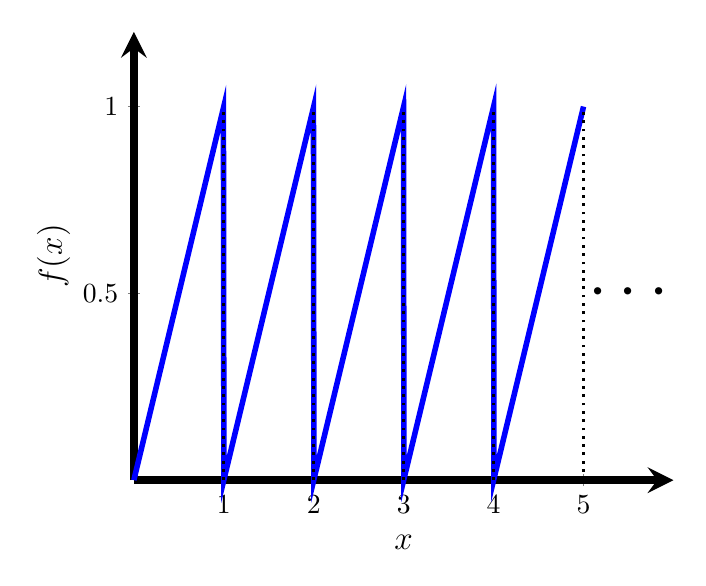
\begin{tikzpicture}
\begin{axis}[
    axis lines=middle,
    axis line style={black, line width=3pt},
    xlabel={\large $x$},
    ylabel={\large $f(x)$},
    xlabel style={at={(axis description cs:0.5,-0.1)},anchor=north},
    ylabel style={at={(axis description cs:-0.1,.5)},rotate=90,anchor=south},
    xmin=0, xmax=6,
    ymin=0, ymax=1.2,
    xtick={0,1,...,5},
    ytick={0,0.5,1},
    samples=1000,
    domain=0:5,
    no markers,
    clip=false,
    yticklabel style={/pgf/number format/fixed},
    after end axis/.code={
        \node at (axis cs:5.5,0.5) {\Huge $\cdots$};
        % Add dotted vertical lines
        \foreach \x in {1,2,3,4,5} {
            \draw [dotted, line width=1pt] (axis cs:\x,0) -- (axis cs:\x,1);
        }
    }
]
\addplot+[blue, line width=2pt, mark=none] expression {mod(x,1)};
\end{axis}
\end{tikzpicture}
\caption[]{\textbf{A sawtooth function with period one.} It is plotted in the usual manner, with a vertical line connecting the points $(k,1)$ and $(k, 0)$ for $k=1, 2, 3, \ldots$, which, in theory, makes it not a function, but in reality, we ignore the vertical lines because they are ``plotting artifacts'' left to guide our eyes.}
\label{fig:SawtoothFunction}
\end{figure}

\subsection*{Working With More Complex Sets}

Let’s build on this with another example, inspired by the \textbf{sawtooth wave} function, $f(x)$, defined as,
\[
f(x) = 
\begin{cases} 
x, & 0 \leq x < 1, \\
x \mod 1, & x \geq 1.
\end{cases}
\]
The goal is to understand sets defined by conditions such as,
\[
S_{\rm B} := \{ x \in (0, \infty) ~\big|~ f(x) = \frac{0.9}{i}, \, i = 1, 2, 3, \ldots \}.
\]

\textbf{Breaking it down:}
For simplicity, let’s first analyze subsets of $S_{\rm B}$ based on intervals of $x$. For example:
    \begin{itemize}
        \item Points in $(0, 1]$ that satisfy $f(x) = \frac{0.9}{i}$ are:
        \[
        S_{{\rm B},1} = \{x \in (0, 1] ~\text{such that}~ x = \frac{0.9}{i}, \, i = 1, 2, 3, \ldots \}.
        \]
        \item Points in $(1, 2]$ that satisfy $f(x) = \frac{0.9}{i}$ are:
        \[
        S_{{\rm B},2} = \{x \in (1, 2] ~\text{such that}~  x = 1 + \frac{0.9}{i}, \, i = 1, 2, 3, \ldots \}.
        \]
        \item Similarly, for $(j-1, j]$, we can write:
        \[
        S_{{\rm B},j} = \{x \in (j-1, j] ~\text{such that}~  x = (j-1) + \frac{0.9}{i}, \, i = 1, 2, 3, \ldots \}.
        \]
    \end{itemize}


\textbf{Key Takeaways}

\begin{enumerate}
    \item \textbf{Set-builder notation} uses conditions to define a set, like restricting a domain or specifying a property.
    \item If you are confused about a set,  writing out many of the ``mysterious symbols'' in your favorite spoken language can be helpful. 
\end{enumerate}

\bigskip

\begin{example}
\label{ex:SetNotationExamples}
Here are some practice problems.

\begin{enumerate}
\renewcommand{\labelenumi}{(\alph{enumi})}
\setlength{\itemsep}{.2cm}
    \item Write in set notation: The set of all positive integers divisible by 3 (same as being a multiple of 3).
    \item Enumerate the elements of the set $T := \{x \in (0, 1] ~\big|~ x = \frac{1}{i}, \, i = 2, 3, 4, \ldots\}$.
    \item Explain what is meant by $\{ n \in \nat ~\big|~ n~~{\rm mod}~ 3 = 0\}$ and then, how is the set different from $\{ n \in \mathbb{Z} ~\big|~ n~~{\rm mod}~ 3 = 0\}$.

\end{enumerate}
\end{example}

\solution

\begin{enumerate}
\renewcommand{\labelenumi}{(\alph{enumi})}
\setlength{\itemsep}{.2cm}
    \item Let’s define the set \(S := \{x \in \mathbb{N} ~\big|~ x = 3k, \, k \in \mathbb{N}\}.\) This means that $S$ contains all positive integers that can be written as a multiple of 3, where $k$ is a positive integer. Enumerating a few elements of $S$, we find
        \[
        S = \{3, 6, 9, 12, \ldots\}.
        \]

    \item The condition $x = \frac{1}{i}$ means that $x$ is the reciprocal of a positive integer $i \geq 2$. Substituting successive values of $i$, we get:
        \[
        T = \left\{\frac{1}{2}, \frac{1}{3}, \frac{1}{4}, \frac{1}{5}, \ldots \right\}.
        \]
Observe that $T$ is infinite, but we can systematically list all its elements, helping us to understand the set.

\item The set $\{ n \in \mathbb{N} ~\big|~ n \mod 3 = 0 \}$ consists of all natural numbers (positive integers) that are divisible by 3. In terms of set notation, this can be written as:
\[
\{ n \in \mathbb{N} ~\big|~ n \mod 3 = 0 \} = \{3, 6, 9, 12, \ldots\}.
\]
This is the set of positive multiples of 3, starting from 3, since $\mathbb{N}$ only includes positive integers.\\

The set $\{ n \in \mathbb{Z} ~\big|~ n \mod 3 = 0 \}$, however, includes all integers divisible by 3, zero as well as positive and negative integers. In terms of set notation, this is,
\[
\{ n \in \mathbb{Z} ~\big|~ n \mod 3 = 0 \} = \{\ldots, -9, -6, -3, 0, 3, 6, 9, \ldots\}.
\]
The key difference is that the first set (with ``domain'' $\mathbb{N}$) only contains positive integers, while the second set (with ``domain'' $\mathbb{Z}$) includes negative integers, zero, and positive integers, representing all integer multiples of 3.
   
\end{enumerate}
\Qed



%%%%%%%%%%%%%%%%

\section{Euler's Formula}
\label{sec:IntroEulerFormula}

He did a lot of stuff, Euler! Somehow, in popular culture, we know some of the famous physicists, such as Newton, Curie, and Einstein, but know little about the mathematicians. Euler is one to know. You can learn more \href{https://en.wikipedia.org/wiki/Leonhard_Euler}{here}, if you wish.

Many of us do not learn Euler's Formula in High School because it comes from Calculus. However, Euler's Formula makes working with complicated trig expressions a breeze, and thus we will cover it now by introducing it as a definition. When we cover Taylor Expansions (McLaurin Expansions), we'll be able to replace the definition with a theorem. 

\begin{tcolorbox}[title=\textbf{Euler's Formula}, breakable, colback=mylightblue]

\begin{definition} 
\label{def:EulerFormula}
Let $\im$ denote $\sqrt{-1}$ (that is, $\im^2 = -1$). Then, for $x \in \real$,
\begin{equation}
    e^{\im x}:= \cos(x) + \im \sin(x).   
\end{equation} 
\end{definition}
    
\end{tcolorbox}

Let's note that $e^{-\im x}=e^{\im (-x)}:= \cos(-x) + \im \sin(-x) =  \cos(x) - \im \sin(x)$, because cosine is an even function (that is,$\cos(-x) = \cos(x)$) and sine is an odd function (that is, $\sin(-x) = -\sin(x)$). Hence, 
$$ e^{\im x} + e^{-\im x} = 2 \cos(x), $$
yielding
\begin{empheq}[box=\bluebox]{equation}
\cos(x) = \frac{ e^{\im x} + e^{-\im x}}{2} .
\end{empheq}
Similarly,
$$ e^{\im x} - e^{-\im x} = 2 \im \sin(x), $$
yielding
\begin{empheq}[box=\bluebox]{equation}
   \sin(x) = \frac{ e^{\im x} - e^{-\im x}}{2 \im}.
\end{empheq}
At first blush, these formulas seem a needless complication of two perfectly manageable functions, $\sin(x)$ and $\cos(x)$. We get it. Do you recall, however, those crazy trig reduction formulas you had to derive and memorize? They can be derived much more easily through Euler's formula. Here is our first example.

\begin{example}
    Derive a simpler formula for $cos^2(x):= \left( \cos(x) \right)^2$.
\end{example}

\textbf{Solution:}
\begin{equation}
\setlength{\jot}{8pt}
\begin{aligned}
\cos^2(x) &= \left(\frac{e^{\im x} + e^{-\im x}}{2}\right)^2 \\ 
&= \frac{e^{\im 2  x} + 2 + e^{-\im 2  x}}{4} \\ 
&= \frac{1}{2} + \frac{1}{2} \frac{ e^{\im2 x} + e^{-\im 2 x}}{2} \\ 
&=  \frac{1}{2} + \frac{1}{2}\cos(2x).
\end{aligned}
\end{equation}
The key ``trick'' is to use the usual exponential rules, so that $e^{\im x} \cdot e^{\im x} = e^{\im 2x}$ and $e^{\im x} \cdot e^{-\im x} = e^{0} = 1$, and so on. 

\Qed

Here is a more complicated example.

\begin{example}
 Use Euler's formula to derive a simpler expression for $\sin^2(x)\cos(x)$. 
\end{example}

\textbf{Solution:}
We start by writing out $\sin(x)$ and $\cos(x)$ in terms of exponential functions and substituting these expressions into $\sin^2(x)\cos(x)$, yielding,
\begin{equation}
\label{eq:EulerExample02}
    \setlength{\jot}{8pt}
\begin{aligned}
    \sin^2(x)\cos(x) &= \left(\frac{e^{\im x} - e^{-\im x}}{\im 2 }\right)^2 \left(\frac{e^{\im x} + e^{-\im x}}{2} \right) \text{ (square the first term)}\\
    &= \frac{(e^{\im 2  x} - 2 + e^{-\im 2  x})(e^{\im x} + e^{-\im x})}{(-4) (2)} \text{ (multiply out the terms)}\\
    &=  \frac{e^{\im 3  x} - 2e^{\im x} + e^{-\im x} +e^{\im x} -2 e^{-\im x}+ e^{-\im 3  x}}{-8} \text{ (add like terms and group)}\\
    &= \frac{ \left( e^{\im x} + e^{-\im x}\right) - \left(e^{\im 3  x} + e^{-\im 3  x}   \right)}{8} \\
    &= \frac{1}{4} \frac{ \left( e^{\im x} + e^{-\im x} \right) }{2}  - \frac{1}{4} \frac{ \left(e^{\im 3  x} + e^{-\im 3  x} \right)}{2}\\
     &= \frac{1}{4}  \cos(x) - \frac{1}{4} \cos(3x).
\end{aligned}
\end{equation}
\Qed


\begin{factColor}{Consequence of Euler's Formula}{factTrigPowers}
Any (finite) product of powers of sines and cosines,
\begin{equation}
\Pi_{k=1}^N \sin^{n_k}(\omega_k x) \cdot \cos^{m_k}(\omega_k x),
\end{equation}
with $n_k$ and $m_k$ positive integers, can be expressed as a linear combination of sines and cosines to the first power, 
\begin{equation}
   a_0 + \sum_{i=1}^J a_i \sin(\nu_i   x) +  \sum_{i=1}^K b_i \cos(\nu_i   x),
\end{equation} 
plus a constant, where the $\nu_i$\,s are sums of $\pm \omega_k$, $1 \le k \le N$. We recall from ROB 101 that linear combinations are always finite.\\

\textbf{Note:} In \eqref{eq:EulerExample02}, $N=1$, $\omega_1=1$, $\nu_1 = \omega_1$ and  $\nu_2 = \omega_1 + \omega_1 + \omega_1 = 3 \omega_1$. \\

\textbf{Note:} See Table~\ref{table:sine-cosine-powers} and Chapter~\ref{sec:BinomialEulerFormula} for a convenient set of power reductions for sine and cosine. 
\end{factColor}

\bigskip

\begin{center}
\setlength{\fboxrule}{2pt}  % Setting the thickness of the border line
   \fbox{\parbox{0.9\linewidth}{\textcolor{blue}{\bf \large You've earned a bit of hilarity because only you, a denizen of Calculus, can even begin to appreciate this video: \href{https://youtu.be/tbqU9APUuYI}{All The Math References Frame by Frame From Animation vs. Math} A link to the un-commented video is in the description. Even your author found the running commentary helpful! The video is deep and a stitch at the same time. \textcolor{black}{Warning: Video Game style of violence, stick figures vs math symbols, no blood}. Includes extra dimensions and time travel.} 
}
} 
\end{center}

\section{Hyperbolic Trig Functions and Relation to Euler's Formula}

The ordinary trigonometric functions arise by studying the unit circle. The \textbf{hyperbolic trigonometric functions} arise from the study of the unit hyperbola. A really great explanation is given in \href{https://youtu.be/Wfpb-fniSSk}{Hyperbolic functions and the unit hyperbola}, from Khan Academy's pre-calculus series. If you become an Aero, Civil, or Mechanical Engineer, you may encounter them daily, as explained in \href{https://youtu.be/Y66Y6ksLP6Y}{The applications of hyperbolic trig: Why do we even care about these things?} by Zach Star. We introduce them here due to their parallels with Euler's formula in Def.~\ref{def:EulerFormula}.

\bigskip

\begin{tcolorbox}[title=\textbf{Hyperbolic Trig Functions}, breakable, colback=mylightblue]

\begin{definition} 
\label{def:HyperbolicTrig}
For all $x \in \real$,
\begin{equation}
\begin{aligned}
    \cosh(x) &:= \frac{e^x+ e^{-x}}{2} \\
    \sinh(x) &:= \frac{e^x - e^{-x}}{2} \\
    \tanh(x) &:= \frac{\sinh(x)}{\cosh(x)} \\
    \href{https://en.wikipedia.org/wiki/Hyperbolic_functions#:~:text=Hyperbolic%20functions%20were%20introduced%20in,Riccati%20and%20Johann%20Heinrich%20Lambert.}{etch}&:= \ldots
\end{aligned}
\end{equation} 
\end{definition}
The functions are called hyperbolic cosine, hyperbolic sine, hyperbolic tangent, and hyperbolic etc. (of course!).     
\end{tcolorbox}

\bigskip

The hyperbolic trig functions play a minor role in this course. We introduce them here to help you digest Euler's Formula. We note that
\begin{equation}
\begin{aligned}
    \cos(x) &= \cosh(\im x) = \frac{ e^{\im x} + e^{-\im x}}{2}\\
    \sin(x) &= \sinh(\im x) = \frac{ e^{\im x} - e^{-\im x}}{2},
\end{aligned}
\end{equation}
even though the hyperbolic functions were discovered before Euler's formula. 

We would be remiss not to mention how the hyperbolic functions show up in Architecture, in the form of the \href{https://en.wikipedia.org/wiki/Catenary_arch}{Catenary Arch}, which is a mainstay of the beautiful buildings by \href{https://en.wikipedia.org/wiki/Antoni_Gaud%C3%AD#:~:text=Quest%20for%20a%20new%20architectural%20language}{Gaudi}. Also, you know that $\sin^2(x) + \cos^2(x) = 1$. The hyperbolic version is
$$\cosh^2(x) \underset{\uparrow}{-} \sinh^2(x)  =  1,$$
(not a typo) as you can multiply out and check for yourself. \\

\begin{table}[ht]
\renewcommand{\arraystretch}{1.5}
\centering
\begin{tabular}{|c|c|c|}
\hline
\textbf{Function} & \textbf{Principal Value} & \textbf{Domain} \\
\hline
\(\acosh(x)\) & \(\acosh(x) = \ln\left(x + \sqrt{x^2 - 1}\right)\) & \(x \geq 1\) \\
\hline
\(\asinh(x)\) & \(\asinh(x) = \ln\left(x + \sqrt{x^2 + 1}\right)\) & All \(x \in \mathbb{R}\) \\
\hline
\end{tabular}
\caption{Principal domains for \(\acosh(x)\) and \(\asinh(x)\).}
\label{tab:PrincipalDomainsHyperbolicInverseFunctions}
\end{table}

\bigskip

\textbf{In case you want to learn more:}
\begin{itemize}
    \item \href{https://youtu.be/m9nwdn55Z2w}{Hyperbolic Trig Identities} by the The Organic Chemistry Tutor.
    \item \href{https://www.youtube.com/watch?v=HnHnEnkZpJA}{Why hyperbolic functions are actually really nice} by Dr. Trefor Bazett.
\end{itemize}




\section{Summing Symbol and Change of Indices}

The summing symbol $\displaystyle \Sigma_{i=1}^{n} x_i $ is shorthand for $x_1 + x_2 + \cdots x_n$. In Julia, it can be implemented with a \texttt{for loop} or with the command \texttt{sum(x)}, if $x$ is a vector with components $x_i$.\\

It is sometimes useful to perform a \textbf{change of index} in a sum. For example, 
\begin{empheq}[box=\bluebox]{equation}
\sum_{i=1}^n (i-1) = \sum_{j=0}^{n-1} j =   \sum_{j=1}^{n-1} j
\label{eqn:ChangeIndexSum}
\end{empheq}
by defining the change of index $j=i-1$. Hence, when $i=1$, its lower limit, $j=0$, and when $i = n$, its upper limit, $j=(n-1)$. The simplification in the third sum is because $j=0$ does not contribute to the sum, so one can remove it.



\section{Binomial Theorem}

The Binomial Theorem typically covered in Algebra II provides a method for expanding $(x+y)^n$, where $x+y$ and $(x+y)^n$ are called \textbf{binomials}. This theorem enables the expansion of the polynomial $(x + y)^n$ into a sum composed of terms of the form $x^{n-k}\cdot y^k$, where $0 \le k \le n$ is an integer. As an example, for $n = 4$, the expansion yields: $(x+y)^4 = x^4 + 4x^3y + 6x^2y^2 + 4xy^3 + y^4$. The coefficient in front of each term $x^{n-k}y^k$ is known as the \textbf{binomial coefficient}, often denoted as $\binom{n}{k}$. 




\subsection{Binomial Coefficients}

In mathematics, binomial coefficients are positive integers that appear as coefficients in the Binomial Theorem. They are denoted by $\binom{n}{k}$, where $n$ and $k$ are integers such that $n\ge  k \ge 0$. These coefficients represent the $x^k$ term in the expansion of $(1 + x)^n$. The binomial coefficients are defined by 
\begin{empheq}[box=\bluebox]{equation}
\label{eqn:BinomialCoeffDef}
    \binom{n}{k} := \frac{n!}{k!(n-k)!},
\end{empheq}
where $!$ denotes factorial; for example, $5! = 5 \cdot 4 \cdot 3 \cdot 2 \cdot 1 = 120$. Equivalently, this formula can be written as
 \begin{equation}
 \binom{n}{k} ={\frac {n \cdot (n-1)\cdots (n-k+1)}{k\cdot (k-1)\cdots 1}}=\prod _{\ell =1}^{k}{\frac {n-\ell +1}{\ell }}=\prod _{\ell =0}^{k-1}{\frac {n-\ell }{k-\ell }},
\end{equation}
each of which is more efficient for doing the actual calculation. 

\begin{rem} By convention, $0!:=1$ and hence $\binom{n}{0}=1$ and $ \binom{n}{n}=1$. 
    
\end{rem}

In the field of combinatorics, these coefficients denote the number of \textbf{distinct ways} that $k$ elements can be selected from a set of $n$ elements. Hence, $\binom{n}{k}$ is frequently pronounced as ``n choose k''.  As an example, if you have a group of five people $(n = 5)$ and you want to select a team of two people $(k = 2)$ from this group, the number of different teams you can form is given by ``5 choose 2'' or $\binom{5}{2}$, which equals 10 according to \eqref{eqn:BinomialCoeffDef}. It is important to note that  $\binom{n}{k}$ doesn't take into account the order of the elements chosen. If the order were important (for instance, if you were choosing a president and a vice president from a group), you would use a different formula (called a permutation) to determine the number of possible distinct combinations of a president and a vice president.

\bigskip

\begin{propColor}{Useful Lower Bound for Studying Euler's Number}{BinomialCoeffBoundLower}
For $n > 2k$,
\begin{equation}
    \label{eq:BinomialCoeffBoundLower}
    \binom{n}{k} := \frac{n!}{k!(n-k)!} = \frac {n \cdot (n-1)\cdots (n-k+1)}{k!} > \frac{n^k}{2^k k!}.
\end{equation} 

\bigskip 

\textbf{Note:} This is a \textbf{lower bound} because $\frac{n^k}{2^k k!} < \binom{n}{k} := \frac{n!}{k!(n-k)!}$. This simple bound will allow us in Chapter~\ref{sec:ExponentialGrowth} to show that exponentials of the form $a^x$, with $a>1$, \textbf{grow faster than any polynomial function} as $x$ tends to infinity.
\end{propColor}

\textbf{Proof:}  From $n > 2k$, we have $\frac{n}{2} > k$ and $-k > -\frac{n}{2} $. Thus, $(n-k+1) > (n - \frac{n}{2} +1) > \frac{n}{2}.$ Hence, $n > (n-1) > \cdots > (n-k+1) > \frac{n}{2}$. Therefore, 
$$
\underbrace{n \cdot (n-1)\cdots (n-k+1)}_{k\text{-times}} >  \frac{n^k}{2^k} \implies \frac {n \cdot (n-1)\cdots (n-k+1)}{k!} > \frac{n^k}{2^k k!}.$$

\Qed

\begin{propColor}{Useful Upper Bounds for Studying Euler's number}{BinomialCoeffBoundUpper}
For all $n\ge 1$ and $0 \le k \le n$,
\begin{equation}
    \label{eq:BinomialCoeffBoundUpperA}
    \binom{n}{k} := \frac{n!}{k!(n-k)!} = \frac {n \cdot (n-1)\cdots (n-k+1)}{k!} \le  \frac{n^k}{k!},
\end{equation} 
and for all $0 < k < n$, the inequality is strict, namely,
\begin{equation}
    \label{eq:BinomialCoeffBoundUpperB}
    \binom{n}{k} := \frac{n!}{k!(n-k)!} = \frac {n \cdot (n-1)\cdots (n-k+1)}{k!} <  \frac{n^k}{k!}.
\end{equation}

\bigskip 

\textbf{Note:} This even simpler bound will help us to approximate Euler's number.
\end{propColor}

% \begin{propColor}{A Useful Upper Bound for Studying Euler's number}{BinomialCoeffBoundUpper}
% For all $n\ge 2$ and $0 < k < n$,
% \begin{equation}
%     \label{eq:BinomialCoeffBoundUpper}
%     \binom{n}{k} := \frac{n!}{k!(n-k)!} = \frac {n \cdot (n-1)\cdots (n-k+1)}{k!} <  \frac{n^k}{k!}.
% \end{equation} 

% \bigskip 

% \textbf{Note:} This even simpler bound will help us to approximate Euler's number.
% \end{propColor}

\textbf{Proof:} Equation  \eqref{eq:BinomialCoeffBoundUpperB} holds because $(n-j) \le n $ for all integers $j \ge 0$. Concerning the strict inequality, for $k=1$, the result is immediate.  For $2 \le  k < n$, we have 
$$\underbrace{(n-k+1)< (n-k +2) < \cdots < (n-1) < n}_{k \text{ terms}},$$
and thus $n \cdot (n-1)\cdots (n-k+1) < n^k$.  Substituting this into \eqref{eq:BinomialCoeffBoundUpperB} proves the result.

\Qed


\begin{propColor}{A Second Useful Upper Bound for Studying Euler's Number}{BinomialCoeffBoundUpper02}
For all $n\ge 1$ and $0\le k \le n$,
\begin{equation}
    \label{eq:BinomialCoeffBoundUpper02}
    \binom{n}{k} \frac {1}{n^{k}} \le  \binom{n+1}{k} \frac {1}{\left(n+1 \right)^k},
\end{equation}
and for $n\ge 2$ and $2\le k \le n$, the inequality is strict, namely,
\begin{equation}
    \label{eq:BinomialCoeffBoundUpper03}
    \binom{n}{k} \frac {1}{n^{k}} <  \binom{n+1}{k} \frac {1}{\left(n+1 \right)^k}.
\end{equation}

\bigskip 

\textbf{Note:} These bounds will help us show that $(1 + \frac{1}{n})^n < (1 + \frac{1}{n+1})^{n+1}$, a property that Bernoulli noted when he discovered $e$.
\end{propColor}

\bigskip

\textbf{Proof:}  We only show \eqref{eq:BinomialCoeffBoundUpper03} and leave the other for the interested learner. For all $n\ge 2$ and $2\le k \le n$, we have 
\begin{equation}
    \label{eq:BinomialCoeffBoundUpper02Proof}
    \begin{aligned}
         \binom{n}{k} \frac {1}{n^{k}} &=   \frac {n \cdot (n-1) \cdot (n-2) \cdots (n-k+1)}{k!~ n^k} \\
         \\
         \binom{n+1}{k} \frac {1}{\left(n+1 \right)^k} &=  \frac {(n+1) \cdot (n+1 -1)\cdot (n+1-2)\cdots (n+1-k+1)}{k!~ (n+1)^k}.
    \end{aligned}   
\end{equation}
We can cancel the common term, $k!$, in the denominators. Then, \eqref{eq:BinomialCoeffBoundUpper03} holds if, and only if,
\begin{align*}
    \frac {n \cdot (n-1) \cdot (n-2) \cdots (n-k+1)}{n^k} &<  \frac {(n+1) \cdot (n+1 - 1) \cdot (n+1-2) \cdots (n+1-k+1)}{(n+1)^k} \\
    & \Updownarrow \\
    \underbrace{\frac{n}{n} \cdot \frac{n-1}{n} \cdot \frac{n-2}{n} \cdots \frac{n-k+1}{n}}_{k~\text{terms}} & < \underbrace{\frac{(n+1)}{(n+1)} \cdot \frac{(n+1) - 1}{(n+1)} \cdot \frac{(n+1)-2}{(n+1)}\cdots \frac{(n+1)-k+1}{(n+1)}}_{k~\text{terms}}.
\end{align*}
But this last inequality is true because, for all $n\ge 1$ and $m \ge 1$,
$$ \frac{n-m}{n} = 1 - \frac{m}{n} <  1 -  \frac{m}{(n+1)} = \frac{(n+1) - m}{(n+1)}.$$
\Qed

\begin{table}[htb!]
\renewcommand{\arraystretch}{1.8} % Adjusts the row height
\centering
\begin{tabular}{|c|c|}
\hline
Binomial & Expansion \\
\hline \hline
$(x+y)^{0}$ & $1$ \\ \hline
$(x+y)^{1}$ & $x+y$ \\  \hline
$(x+y)^{2}$ & $x^{2}+2xy+y^{2}$ \\ \hline
$(x+y)^{3}$ & $x^{3}+3x^{2}y+3xy^{2}+y^{3}$ \\ \hline
$(x+y)^{4}$ & $x^{4}+4x^{3}y+6x^{2}y^{2}+4xy^{3}+y^{4}$ \\ \hline
$(x+y)^{5}$ & $x^{5}+5x^{4}y+10x^{3}y^{2}+10x^{2}y^{3}+5xy^{4}+y^{5}$ \\ \hline
$(x+y)^{6}$ & $x^{6}+6x^{5}y+15x^{4}y^{2}+20x^{3}y^{3}+15x^{2}y^{4}+6xy^{5}+y^{6}$ \\ \hline
$(x+y)^{7}$ & $x^{7}+7x^{6}y+21x^{5}y^{2}+35x^{4}y^{3}+35x^{3}y^{4}+21x^{2}y^{5}+7xy^{6}+y^{7}$ \\ \hline
$(x+y)^{8}$ & $x^{8}+8x^{7}y+28x^{6}y^{2}+56x^{5}y^{3}+70x^{4}y^{4}+56x^{3}y^{5}+28x^{2}y^{6}+8xy^{7}+y^{8}$ \\
\hline
\end{tabular}
\caption{A handy list of binomial expansions. Note the symmetry in the coefficients about the middle of each formula. This is because $\binom{n}{k} = \binom{n}{n-k}$.}
\label{tab:BinomialExpansion}
\end{table}

\subsection{Expansion of \texorpdfstring{$(x + y)^n$}{(x + y)n}}
%\texorpdfstring{$(x + y) ^n}$}{(x + y) ^n}}

\begin{thmColor}{Binomial Theorem}{binomialTheoremGeneralN} 
For all integers $n\ge 1$,

\begin{equation}
\begin{aligned}
    (x+y)^{n}&=\sum _{k=0}^{n}\binom{n}{k}x^{n-k}y^{k} \\
    &=\sum _{k=0}^{n}\binom{n}{k}x^{k}y^{n-k}.
\end{aligned}
\end{equation}
Early on, the ``summing notation'' can be a bit much to digest. We note that the above can also be written as
 $$ (x+y)^{n}=\binom{n}{0}x^{n}y^{0}+\binom{n}{1}x^{n-1}y^{1}+\binom{n}{2}x^{n-2}y^{2}+\cdots +\binom{n}{n-1}x^{1}y^{n-1}+\binom{n}{n}x^{0}y^{n}.$$\\

 Table~\ref{tab:BinomialExpansion} provides explicit expansions for $0 \le n \le 8$. A proof by induction is given by \href{https://en.wikipedia.org/wiki/Binomial_theorem#:~:text=the%20binomial%20theorem.-,Inductive%20proof,-%5Bedit%5D}{Wikipedia}, \href{https://www.khanacademy.org/math/in-in-grade-11-ncert/x79978c5cf3a8f108:binomial-theorem/x79978c5cf3a8f108:intro-to-the-binomial-theorem/v/binomial-theorem}{Khan Academy}, \href{https://www.mathsisfun.com/algebra/binomial-theorem.html}{Math is Fun}, and many other sources.
    
\end{thmColor}

\bigskip

\begin{example}
\label{ex:BinomialFor1PlusX}
 Use the Binomial Theorem to determine the expansion of $(1 + x)^n$.
    
\end{example}

\textbf{Solution:} 

\begin{align*}
(1+x)^{n} = (x+1)^n &= \sum_{k=0}^{n}\binom{n}{k}x^{k} \\
&= \binom{n}{0}x^{0} + \binom{n}{1}x^{1} + \binom{n}{2}x^{2} + \binom{n}{3}x^{3} +\cdots + \binom{n}{n-1}x^{n-1} + \binom{n}{n}x^{n} \\
&= 1 + nx + \frac {n(n-1)}{2}x^{2} + \frac {n(n-1)(n-2)}{6}x^{3} + \cdots + nx^{n-1} + x^{n}.
\end{align*}
\Qed



\section{Some Special Functions}


\begin{figure}[htb!]%
\centering
\subfloat[]{%
	\centering
		\setlength{\fboxsep}{0pt}%
\includegraphics[width=0.45\columnwidth]{graphics/Chap01/unitStepFunctionSuperCorrect.png}}%
\hspace{5pt}%
\subfloat[]{%
	\centering
\includegraphics[width=0.45\columnwidth]{graphics/Chap01/unitStepFunction.png}}%
\newline
\subfloat[]{%
	\centering
		\setlength{\fboxsep}{0pt}%
\includegraphics[width=0.45\columnwidth]{graphics/Chap01/unitRectangleFunction.png}}%
\hspace{5pt}%
\subfloat[]{%
	\centering
\includegraphics[width=0.45\columnwidth]{graphics/Chap01/unitTriangleFunction.png}}%
\caption[]{Some useful functions. (a) The unit step function. Here, the graph is done ``by the book'', defining clearly a value of the function at the point of discontinuity, the origin. (b) This is how the unit step function is normally plotted (graphed). You are expected to understand that while you must choose a SINGLE value for the function at the origin, it is usually not important what value you assign at the point of discontinuity. (c) The unit rectangle function is plotted in a ``hybrid manner'' so that its rectangular shape is evident. Normally, one does not care what value is assigned at each of the two points of discontinuity. (d) The unit triangle function is continuous everywhere (it has no jumps). Note the base of the unit rectangle function has a width of one, while the base of the until triangle function has a width of two. \textbf{This is done so that each function's ``shape'' encloses ``unit area'' , meaning the area is one}. }
    \label{fig:SpecialFunctions}
\end{figure}

Figure~\ref{fig:SpecialFunctions} shows three functions, the \href{https://en.wikipedia.org/wiki/Heaviside_step_function}{Unit Step Function} (aka, Heaviside function, or Heaviside unit step function) in (a) and (b), the \href{https://en.wikipedia.org/wiki/Rectangular_function}{Unit Rectangle Function} (aka, rectangular function) in (c), and the \href{https://en.wikipedia.org/wiki/Triangular_function#:~:text=References-,Triangular%20function,-14%20languages}{Unit Triangle Function} (aka, triangular function, hat function, or tent function)  in (d). The functions are defined as follows:\\

\textbf{Unit Step:}
\begin{equation}
    \label{eq:UnitStep}
    \ustep(x):= \begin{cases} 1 & x \ge 0 \\
    0 & x < 0.        
    \end{cases}
\end{equation}

\textbf{Unit Rectangle:}
\begin{equation}
    \label{eq:UnitRectangle}
    {\rm rect}(x):= \begin{cases} 1 & |x| \le \frac{1}{2} \\
    0 & \text{otherwise};       
    \end{cases}
\end{equation}
the area under the function is equal to one because the base and height are both equal to one.

\textbf{Unit Triangle:}
\begin{equation}
    \label{eq:UnitTriangle}
    {\rm tri}(x):= \begin{cases} 1 - |x| & |x| \le 1\\
    0 & \text{otherwise};       
    \end{cases}
\end{equation}
the area under the function is also equal to one because the base of the triangle is equal to two, and the height is equal to one.

\begin{figure}[htb!]%
\centering
\subfloat[]{%
	\centering
		\setlength{\fboxsep}{0pt}%
\includegraphics[width=0.45\columnwidth]{graphics/Chap01/shiftedFunction.png}}%
\hspace{5pt}%
\subfloat[]{%
	\centering
\includegraphics[width=0.45\columnwidth]{graphics/Chap01/TriangleNominal.png}}%
\newline
\subfloat[]{%
	\centering
		\setlength{\fboxsep}{0pt}%
\includegraphics[width=0.45\columnwidth]{graphics/Chap01/TriangleShiftby2.png}}%
\hspace{5pt}%
\subfloat[]{%
	\centering
\includegraphics[width=0.45\columnwidth]{graphics/Chap01/TriangleShiftbyminus2.png}}%
\caption[]{Shifted functions. (a) In blue is shown the nominal function and in red, the function shifted by $x_0 = 6$. Because $x_0>0$, the function's graph is shifted to the right. The shape of the function is preserved. (b) A unit triangle function. (c) The unit triangle function has been shifted to the right by $x_0=2 >0$. (d) The unit triangle function has been shifted to the left by two because $x_0=-2 <0$. Note that the area under the triangles has not changed under shifting because their shape remains the same: their bases are the same, and their heights are the same. The same is true for rectangles.}
    \label{fig:ShiftedFunctions}
\end{figure}

\section{Shifting and Scaling}
\label{sec:ShiftScale}

Shifting and scaling are common ways to create new functions from existing functions. Let $f:\real \to \real$ be some function that you already have in hand. And let $x_0$ and $c \neq 0$ be two real constants.\\

\textbf{The shift of $f(x)$ by $x_0 $} is denoted $f(x-x_0)$. As illustrated in Fig.~\ref{fig:ShiftedFunctions}, the shift operation applied to a function shifts its graph to the right by $x_0$, when $x_0 >0$ and to the left by $|x_0|$, when $x_0 < 0$.

\bigskip
\begin{example}
    Show that with the exception of $x = \pm \frac{1}{2}$, the two points of discontinuity of the rectangle function, we have
    $${\rm rect}(x) = \ustep(x+\frac{1}{2}) -  \ustep(x- \frac{1}{2}). $$
\end{example}
\textbf{Solution:}
For $x< - \frac{1}{2} $, we have $x+\frac{1}{2} <0$ and $x-\frac{1}{2} <0$ and thus $\ustep(x+\frac{1}{2}) -  \ustep(x- \frac{1}{2})= 0 - 0 = 0$, which is the value of ${\rm rect}(x)$. Similarly, for $x> \frac{1}{2} $, we have $x+\frac{1}{2} >0$ and $x-\frac{1}{2} >0$ and thus $\ustep(x+\frac{1}{2}) -  \ustep(x- \frac{1}{2})= 1 - 1 = 0$, which is also the value of ${\rm rect}(x)$. Finally, we consider $-\frac{1}{2} < x < \frac{1}{2} $. Then,  we have $x+\frac{1}{2} >0$ and $x-\frac{1}{2} <0$ and thus $\ustep(x+\frac{1}{2}) -  \ustep(x- \frac{1}{2})= 1 - 0 = 1$, which is the value of ${\rm rect}(x)$.\\

\textbf{Note:} For  $x= - \frac{1}{2} $, we have $\ustep(x+\frac{1}{2}) -  \ustep(x- \frac{1}{2})= \ustep(0) -  \ustep(- 1)= 1 - 0 = 1$, which is the value of ${\rm rect}(-\frac{1}{2})$, but for $x=  \frac{1}{2} $, we have $\ustep(x+\frac{1}{2}) -  \ustep(x- \frac{1}{2})= \ustep(1) -  \ustep(0)= 1 - 1 = 0$, which is NOT the value of ${\rm rect}(\frac{1}{2})$.

\Qed

\bigskip
\textbf{The scale of $f(x)$ by $c \neq 0 $} is denoted $f(c \cdot x)$. As illustrated in Fig.~\ref{fig:ScaledFunctions}, the scale operation applied to a function ``squeezes'' its graph when $c>1$ and expands its graph, when $0 < c < 1$. We are not defining here the scaling operation for negative values of $c$ because it also ``flips'' the function about the $y$-axis. 


\begin{figure}[htb!]%
\centering
\subfloat[]{%
	\centering
		\setlength{\fboxsep}{0pt}%
\includegraphics[width=0.48\columnwidth]{graphics/Chap01/scaledRectangleFunctionNominal.png}}%
\hspace{5pt}%
\subfloat[]{%
	\centering
 \includegraphics[width=0.48\columnwidth]{graphics/Chap01/SineFunctionNominal.png}}%
\hspace{5pt}%
\subfloat[]{%
	\centering
 \includegraphics[width=0.48\columnwidth]{graphics/Chap01/scaledRectangleFunction2x.png}}%
\hspace{5pt}%
\subfloat[]{%
	\centering
\includegraphics[width=0.48\columnwidth]{graphics/Chap01/SineFunction2x.png}}%
\hspace{5pt}%
\subfloat[]{%
	\centering
 \includegraphics[width=0.48\columnwidth]{graphics/Chap01/scaledRectangleFunctionHalfx.png}}%
\hspace{5pt}%
\subfloat[]{%
	\centering
\includegraphics[width=0.48\columnwidth]{graphics/Chap01/SineFunctionHalfx.png}}%
\caption[]{Scaled functions. (a) Unit rectangle function in blue. (c) Unit rectangle function scaled by $c=2$ in red. The area of the rectangle has been decreased by a factor of two. (e) Unit rectangle function scaled by $c=\frac{1}{2}$ in black. The area of the rectangle has been increased by a factor of two. (b) Two periods of the function $\sin(x)$ in blue. (d) Two periods of the function $\sin(2 x)$ in red. The frequency has been doubled. (f) Two periods of the function $\sin(\frac{x}{2})$. The frequency has been halved. }
    \label{fig:ScaledFunctions}
\end{figure}



% \begin{figure}[htb!]%
% \centering
% \subfloat[]{%
% 	\centering
% 		\setlength{\fboxsep}{0pt}%
% \includegraphics[width=0.31\columnwidth]{graphics/Chap01/scaledRectangleFunctionNominal.png}}%
% \hspace{5pt}%
% \subfloat[]{%
% 	\centering
% \includegraphics[width=0.31\columnwidth]{graphics/Chap01/scaledRectangleFunction2x.png}}%
% \hspace{5pt}%
% \subfloat[]{%
% 	\centering
% \includegraphics[width=0.31\columnwidth]{graphics/Chap01/scaledRectangleFunctionHalfx.png}}%
% \newline
% \subfloat[]{%
% 	\centering
% \includegraphics[width=0.31\columnwidth]{graphics/Chap01/SineFunctionNominal.png}}%
% \hspace{5pt}%
% \subfloat[]{%
% 	\centering
% \includegraphics[width=0.31\columnwidth]{graphics/Chap01/SineFunction2x.png}}%
% \hspace{5pt}%
% \subfloat[]{%
% 	\centering
% \includegraphics[width=0.31\columnwidth]{graphics/Chap01/SineFunctionHalfx.png}}%
% \caption[]{Scaled functions. (a) Unit rectangle function in blue. (b) Unit rectangle function scaled by $c=2$ in red. The area of the rectangle has been decreased by a factor of two. (c) Unit rectangle function scaled by $c=\frac{1}{2}$ in black. The area of the rectangle has been increased by a factor of two. (d) Two periods of the function $\sin(x)$ in blue. (e) Two periods of the function $\sin(2 x)$ in red. The frequency has been doubled. (c) UTwo periods of the function $\sin(\frac{x}{2})$. The frequency has been halved. }
%     \label{fig:ScaledFunctions}
% \end{figure}

\bigskip
\begin{example}
    Compute the area under the functions,
    \begin{enumerate}
\renewcommand{\labelenumi}{(\alph{enumi})}
\setlength{\itemsep}{.2cm}
\item $\rect(x)$
\item $\rect(3x)$
\item $\rect(0.2 x)$
\item $2 \cdot \tri(x)$
\item $2 \cdot \tri(11x)$
\item $2 \cdot \tri(\frac{x}{3})$
\end{enumerate}
\end{example}
\textbf{Solutions:}

    \begin{enumerate}
\renewcommand{\labelenumi}{(\alph{enumi})}
\setlength{\itemsep}{.2cm}
\item $\rect(x)$ has a base of one and a height of one, and thus its area is also one, i.e., $1.0$.
\item $\rect(3x)$ has a base of one-third and a height of one, and thus its area is one-third, i.e., $\frac{1}{3}$.
\item $\rect(0.2 x)$ has a base of five and a height of one, and thus its area is five, i.e., $5.0$.
\item $2 \cdot \tri(x)$ has a base of two and a height of two, and thus its area is two (one half base times height), i.e., $2.0$.
\item $2 \cdot \tri(11x)$ has a base of two-elevenths and a height of two, and thus its area is $\frac{2}{11}$.
\item $2 \cdot \tri(\frac{x}{3})$ has a base of six and a height of two, and thus its area is six, i.e., $6.0$.
\end{enumerate}


\Qed


\begin{figure}[htb]%
\centering
\subfloat[]{%
\includegraphics[width=0.45\columnwidth]{graphics/Chap01/OpenLoopNoDisturbance.png}}%
\hfill
\subfloat[]{%
\raisebox{0.55cm}{\includegraphics[width=0.55\columnwidth]{graphics/Chap01/OpenLoopWithDisturbance.png}}}%
\hfill
\newline
\subfloat[]{%
	%\centering
\includegraphics[width=0.7\columnwidth]{graphics/Chap01/ClosedLoopDiagramWithDisturbance.png}
}%
\hfill%
    \caption[]{Feedback diagrams, where $P$ stands for plant, which is the generic name for the system that is to be controlled (e.g., motor with a link connected to it), $y$ is the measured output (e.g. joint angle), $u$ is the input to the plant (e.g., motor torque), and $d$ is a disturbance signal, also called a perturbation (e.g, friction in the joint). (a) An open-loop system without a disturbance. (b) An open-loop system with a disturbance. (c) A \textbf{closed-loop system}, where $K$ is the \textbf{controller gain}, $r$ is the reference signal (what we want $y$ to become), and $e$ is the error term, the difference between the reference signal and the measured output. In (a) and (b), there is no loop, hence the term ``open-loop system'', while in (c), a loop is present, hence the term ``closed-loop control''. \textbf{Credit for this idea: Prof. Semyon Meerkov, University of Michigan, ECE Department}. }
    \label{fig:FeedbackDiagramsStatic}
\end{figure}



\section{A Peek at Feedback Control and a Partial Roadmap to this Textbook} 

Why feedback control and why in a Chapter on Pre-Calculus: 
\begin{itemize}
\item Feedback control is a pervasive technology. In Michigan Engineering, feedback control courses can be found in approximately half of its departments. Its widespread representation rivals Physics and Mathematics.

    \item The robot arms in Fig.~\ref{fig:RobotAbsoluteAngle} are not worth much if you cannot command them to reach an object at a given position. In many cases, that comes down to regulating each of the joints in the robot arm to a particular value, called a \textbf{setpoint}. Commanding robot joints to setpoints is the bread-and-butter of feedback control. Because some of the key ideas only involve basic algebra, pre-calculus knowledge is enough to glean key insight into how a feedback controller works.

    \item The description of a feedback control system will also allow us to highlight where Calculus is used in Robotics, partially giving you a roadmap to this textbook. 
\end{itemize}

Consider Fig.~\ref{fig:FeedbackDiagramsStatic}-(b). The diagram represents the algebraic equation
\begin{empheq}[box=\bluebox]{equation}
y = P \cdot u + d,
\end{empheq}
where 
\begin{itemize}
    \item $P>0$ is a positive constant representing the \textbf{gain} (aka, multiplying factor) of the system to be controlled or regulated; let's imagine that our plant is one of the links in Fig.~\ref{fig:robotKinematicChain} attached to a DC motor. Our objective is to regulate the joint angle to a desired value, which we will denote by $r$ because, in the control community, we call it a \textbf{reference signal}.
    \item $u$ is the \textbf{input or control signal} to the plant, a signal we can manipulate to achieve our goal; let's imagine that $u$ is the torque of the DC motor. 
    \item $y$ is the  \textbf{measured output} of the system; let's imagine it is the output of the encoder at the joint angle. 
    \item $d$ is our nemesis, called a \textbf{disturbance signal} or \textbf{perturbation} in control parlance, which is universally present in real life; let's imagine that $d$ is friction in the joint of the robot. In industrial robots, unfortunately, $d$ can be very large. Yes, manufacturers try to minimize it, but alas, that is hard and expensive.  
\end{itemize}

\bigskip

\emstat{
\textbf{How to Read the Diagrams in Fig.~\ref{fig:FeedbackDiagramsStatic}}: These diagrams represent linear equations. In (a), $y = P \cdot u$, whatever signal comes into the box is multiplied by the system gain $P$. In (b), the circle with the plus signs is called a \textbf{summing junction} aka \textbf{summer}; the output of the summing junction is equal to the sum of all the signals that enter it, with each input signal weighted by the sign nearest to it. Because in (b), they are all plus signs,  $y = P \cdot u + d$. In (c), we have our first encounter with a feedback system, aka a closed-loop system. The first summer represents $e = r - y$, and the second summer represents $y = P \cdot u + d$, as in (b). These two equations are connected by $u = Ke$. We will solve these simultaneous equations shortly, but not now!
} % end emstat

\bigskip

\textbf{\Large Objective:} Regulate $y$ to $r$, a desired angle, despite us not being able to measure the disturbance, $d$. 

\bigskip

\subsubsection{Open-loop Approach to the Problem}
We know the plant model is $y = P \cdot u + d$, and we cannot measure $d$. So we propose 
\begin{equation}
u = K \cdot r
\end{equation}
and seek to select $K$ so that $y \approx r$, it's desired value. We write this as
\begin{equation}
r \approx y = P \cdot u + d = P \cdot K \cdot r + d.
\end{equation}
Because we know nothing about $d$, we assume it is as likely to be positive as negative, with a mean value of zero. This leads to 
\begin{equation}
r \approx y \iff P \cdot K = 1 \iff K = \frac{1}{P},
\end{equation}
that is, the control gain is set to the reciprocal of the plant gain. Because $P \cdot K =1$, our open-loop control system results in 
\begin{equation}
y =r + \bm{d}.
\end{equation}
There are two issues with this solution:
\begin{enumerate}
\renewcommand{\labelenumi}{(\alph{enumi})}
\setlength{\itemsep}{.2cm}
    \item the disturbance passes directly through to the output, causing error in the precision of the control system; and
    \item we may not know the plant gain exactly, and hence our control gain is really $K = \frac{1}{P^{\rm nom}}$, a nominal value for the plant gain, and the real output is then
    $$y = \left(\frac{P}{P^{\rm nom}} \right) \cdot r+ \bm{d}. $$
\end{enumerate}
There must be a better way to handle the uncertainty in the model, namely, the unmeasurable disturbance and any variations in the plant gain, $P$. Right?

\subsubsection{Closed-loop Approach to the Problem}

The feedback diagram in Fig.~\ref{fig:FeedbackDiagramsStatic}-(c) yields 
\begin{equation}
\label{eq:FeedbackEquationsStatic}
    \begin{aligned}
        y &= P \cdot u + d \\
        e &= r - y \\
        u & = K\cdot e,
    \end{aligned}
\end{equation}
where $K$ is a feedback gain. We get to adjust it so as to best meet our objective of making the output as close to the commanded reference value as possible, that is, $y \approx r$. Combining the bottom two equations of \eqref{eq:FeedbackEquationsStatic}, we have 
$$ u = K\cdot e = K\cdot (r - y).$$
Plugging this into the top equation yields
$$ y = P \cdot  K\cdot e = P \cdot K\cdot \left(  r - y \right) + d, $$
a scalar linear equation. Solving for $y$ gives us
$$ (1 + P \cdot K) \cdot y = P \cdot K \cdot r + d,$$
and thus,
\begin{equation}
    y = \frac{P \cdot K }{1 + P \cdot K}\cdot r + \frac{1}{1 + P \cdot K} \cdot d,
\end{equation}
a linear equation relating the reference signal, $r$, and the disturbance signal, $d$, to the output, $y$.
\textbf{This is the most important equation in feedback control} because it tells us everything about how the free parameter $K$ in the controller relates to the multiplying factor in front of the reference command, namely, $\frac{P \cdot K }{1 + P \cdot K}$, and in front of the disturbance, namely  $\frac{1}{1 + P \cdot K}$. 

In a ``perfect world'', we would have $\frac{P \cdot K }{1 + P \cdot K} = 1$ and $\frac{1}{1 + P \cdot K} = 0$, so that $y = r$. Perfection is hard to achieve, so we seek to make the following approximations 
$$  \frac{P \cdot K }{1 + P \cdot K} \approx 1 \text{ and } \frac{1}{1 + P \cdot K} \approx 0$$
hold as closely as we can.

\begin{itemize}
    \item Suppose that $P$ has a nominal value of $2$, and we select $K=25$. Then, plugging in values gives us
$$ y = \frac{50}{51} \cdot r + \frac{1}{51} \cdot d \approx 0.98 r + 0.0196 d.$$
The disturbance is greatly attenuated, and $y$ is within 2\% of its desired value, $r$. Not bad, huh?

\item Suppose that $P$ could vary between $1 \le P \le 3$, and we keep $K=25$. Then we have 
\begin{align*}
    y \approx&  0.96 r + 0.0385 d ~~P=1\\
    y \approx&  0.99 r + 0.0136 d ~~P=3,
\end{align*}
which is also great! 
\end{itemize}

\textbf{Note:} Suppose you could select $K=100$. How would the above numbers change? 

\subsubsection{Taking Stock}

Closed-loop control is a game changer. It allows one to  ``track'' reference commands, that is, drive $y$ to its desired value $r$, even in the face of
\begin{itemize}
    \item uncertainty in the mathematical model of the system being controlled, and
    \item nefarious disturbances trying to prevent us from achieving our tracking objective.
\end{itemize}

\subsubsection{Where's the Calculus?}
Nowhere to be seen. Yet! In the above, we've assumed the system to be controlled can be represented by a constant gain, $P$. You know full well that ``$F = ma$'' has to enter into the picture when dealing with a robot. That is called \textbf{dynamics}, and that's where Calculus first comes in. 
\begin{itemize}
\item In Chapter~\ref{sec:ApplicationsDefiniteIntegral}, we will draw on your knowledge of Physics to compute the displacement of an object from its speed of motion, using definite integration. Further applications of integration allow us to compute the mass of a robot link from its density and shape, and its ``center of gravity'', aka ``center of mass'', the point at which a single point mass can summarize the overall effect of gravity on the object. 
    \item In Chapter~\ref{chap:Differentiation}, we'll study derivatives and realize that velocity is the derivative of position with respect to time. In a similar manner, acceleration is the derivative of velocity with respect to time.
    \item Deriving dynamical models of robots via $F = ma$ is very tedious. Lagrange invented another method for creating dynamical models of collections of rigid bodies, such as our 3-link robot. It involves potential energy and kinetic energy. Chapter~\ref{sec:LagrangianDynamics} explores Lagrange's Equations of Motion.
    \item In Chapter~\ref{chap:ODEs}, we will learn about ordinary differential equations (ODEs for short) and how to solve them. We'll also learn how to develop linear approximations of complicated nonlinear differential equations, opening up their analysis to undergraduate students.
    \item In Chapter~\ref{chap:LaplaceTransformFeedbackControl}, we study the Laplace transform, a means to understand the stability of ODEs. The Laplace Transform is a kind of superpower: it transforms linear ODEs into algebraic equations! Yes, really. By looking at the roots of the resulting algebraic equations, we can determine if small perturbations introduced into an ODE model of a robot eventually dissipate (this is what stability is all about) or cause the system to explode (this is the essence of instability). 
    \item In Chapter~\ref{chap:LaplaceTransformFeedbackControl}, we'll use all of this knowledge to design feedback control laws for linear ODEs, culminating in us stabilizing the \href{https://github.com/michiganrobotics/rob311}{BallBot}. If you really like this material, at Michigan, you would follow up with one of EECS 460 Control Systems Analysis and Design, ME 461 Automatic Control, or AEROSP 345 Flight Dynamics and Control. And then there are the \href{https://controls.engin.umich.edu/control-courses/}{graduate-level courses}! Their cardinality is a good approximation of infinity, which may sound intimidating, but it really means that in any given semester, you have a smorgasbord of interesting courses to consider.
\end{itemize}

\bigskip

\section{(Optional Read:) Binomial Theorem meets Euler}

On the surface, the Binomial Theorem, which expands $(x + y)^n$, seems to be limited to helping us with polynomials. However, Euler's number involves $\left(1 + \frac{1}{n} \right)^n$ and Euler's formula allows us to write $\cos^n(x) = \left( \frac{e^{\im x} + e^{-\im x}}{2}  \right)^n$ and  $\sin^n(x) = \left( \frac{e^{\im x} - e^{-\im x}}{2 \im}  \right)^n$. Here, we apply the Binomial Theorem to understand these quantities. 

\subsection{Binomial Theorem meets Euler's Constant}
\label{sec:BinomialMeetsEuler}

% \begin{equation}
% \begin{aligned}
%     \left(1 + \frac{1}{n}\right)^n &= \sum_{k=0}^{n} \binom{n}{k} \left(\frac{1}{n}\right)^k\\
%     &=  1 + n\left( \frac{1}{n} \right) + \frac {n(n-1)}{2}\left( \frac{1}{n} \right)^{2} + \frac {n(n-1)(n-2)}{6}\left( \frac{1}{n} \right)^{3} + \cdots + n\left( \frac{1}{n} \right)^{n-1} + \left( \frac{1}{n} \right)^{n} \\
%     &= \frac{1}{0!} + \frac{1}{1!} + \frac{1}{2!} - {\RED \frac{1}{2!}\frac{1}{n} } + \frac{1}{3!} - {\RED \frac{1}{2n} + \frac{1}{3n^2}}  + \cdots +  {\RED n\left( \frac{1}{n} \right)^{n-1} + \left( \frac{1}{n} \right)^{n}}\\
%     & = \frac{1}{0!} + \frac{1}{1!} + \frac{1}{2!} + \frac{1}{3!} + \cdots - {\RED \frac{1}{2!}\frac{1}{n} + {\RED \frac{1}{2n} + \frac{1}{3n^2}}  + \cdots +  {\RED n\left( \frac{1}{n} \right)^{n-1} + \left( \frac{1}{n} \right)^{n}} } 
% \end{aligned}
% \end{equation}

Applying the Binomial Theorem to the expression $\left(1+{\frac {1}{n}}\right)^{n}$ yields another means to compute Euler's number, $e$. Indeed,
\begin{empheq}[box=\bluebox]{equation}
\left(1+{\frac {1}{n}}\right)^{n}=\sum_{k=0}^n \binom{n}{k}\frac{1}{n^k}.
\end{empheq}
The kth term of this sum is
\begin{equation}
    \begin{aligned}
        \binom{n}{k}{\frac {1}{n^{k}}}&= \frac{n!}{k! (n-k)!} \cdot {\frac {1}{n^{k}}}\\
        & = {\frac {1}{k!}}\cdot {\frac {n \cdot (n-1) \cdot (n-2)\cdots (n-k+1)}{n^{k}}} \\
        & = \frac {1}{k!} \cdot \frac{n}{n} \cdot \frac{n-1}{n} \cdot \frac{n-2}{n} \cdots \frac{n-k+1}{n}\\
        & = \frac {1}{k!} \cdot \left(1 - \frac {1}{n}   \right) \cdot \left(1 - \frac {2}{n}   \right) \cdots \left(1 - \frac {k+1}{n}   \right),
    \end{aligned}
\end{equation}
where we noted that $\frac{n}{n}=1$, $\frac{n-1}{n}=1 -\frac{1}{n}$, $\frac{n-2}{n}=1 -\frac{2}{n}$, all the way to $\frac{n-k+1}{n}=1 -\frac{k+1}{n}$.\\ 

We will now make some approximations in the ``spirit of Calculus'' that will become more rigorous in the next Chapter; you can also see \href{https://en.wikipedia.org/wiki/Binomial_theorem#:~:text=Series%20for%20e,by%20the%20formula}{Wikipedia}. \\

For $k$ fixed and ``$n$ much larger than $k$'', $1 - \frac {1}{n} \approx 1$, $1 - \frac {2}{n}  \approx 1$, all the way to $1 - \frac {k+1}{n}  \approx 1$. If you are with us so far, then you won't mind the next approximation, namely, the product of terms that are close to one is also close to one,  
$$ \left(1 - \frac {1}{n}   \right) \cdot \left(1 - \frac {2}{n}   \right) \cdots \left(1 - \frac {k+1}{n}   \right) \approx 1.$$ 
Therefore, for $k$ constant and ``$n$ large'',
$$\binom{n}{k}{\frac {1}{n^{k}}} \approx {\frac {1}{k!}}.$$
This indicates that $e$ can be approximated as 
\begin{empheq}[box=\bluebox]{equation}
 e \approx \left(1+{\frac {1}{n}}\right)^{n}=\sum_{k=0}^n \binom{n}{k}\frac{1}{n^k} \approx \sum _{k=0}^{n }{\frac {1}{k!}}={\frac {1}{0!}}+{\frac {1}{1!}}+{\frac {1}{2!}}+{\frac {1}{3!}}+\cdots + \frac {1}{n!},
 \end{empheq}
with the approximation becoming better and better as $n$ gets larger and larger. The notion of approximations improving for large $n$ will lead us to the concept of limits in Chapter~\ref{chap:Foundations}. \\

Now, after all these approximations, what do we have? Table~\ref{tab:ComparisoncomputationEulerConstant} compares our two approximations for Euler's number. We see that the sum, $\sum_{k=0}^{n}\frac{1}{k!}$, ``converges'' to $e$ much faster than the product, $\left(1+{\frac {1}{n}}\right)^{n}$. Euler's name is attached to the constant $e$ because he proved rigorously\footnote{Here, ``rigorously'' means that Euler filled in all the holes in the argument we sketched out. In mathematics, rigor refers to a level of thoroughness and consistency in reasoning that ensures the validity and correctness of results. It involves precise definitions, clear assumptions, and sound logical techniques to establish the truth of mathematical statements. Rigor helps in avoiding errors, clarifying concepts, and ensuring that the conclusions reached are reliable and trustworthy. Through rigorous processes, mathematicians aim to build a solid foundation for the development of mathematical theories and the advancement of the field. Engineering is built upon these solid foundations.}, among other things, that as $n$ tends to infinity, the sum converges to $e$.


\begin{table}[hbt]
\centering
\begin{tabular}{|c|c|c|}
\hline 
$n$ & $(1+\frac{1}{n})^n$ & $\sum_{k=0}^{n}\frac{1}{k!}$ \\
\hline \hline
5  & 2.48832000 & 2.71666667 \\ 
\hline
10 & 2.59374246 & 2.71828180 \\
\hline
$10^2$ & 2.70481383 & 2.71828183\\
\hline
$10^3$ & 2.71692393 & 2.71828183 \\
\hline
\end{tabular}
\caption{Comparison of the values of $e \approx 2.71828183 \ldots$, the product $(1+\frac{1}{n})^n$, and the sum $\sum_{k=0}^{n}\frac{1}{k!}$ for various $n$. Values are shown to 8 significant digits. The sum seems to converge must faster, meaning that it provides a more practical way of computing $e$.}
\label{tab:ComparisoncomputationEulerConstant}
\end{table}

\begin{lstlisting}[language=Julia,style=mystyle]
n=100

e_approxA = (1+1/n)^n

e_approxB = 0.0
for k = 0:n
    e_approxB = e_approxB + 1/factorial(big(k))
    # big(k) needed for 21! and beyond
end
[e_approxA; e_approxB; exp(1)]
\end{lstlisting}
\textbf{Output} 
\begin{verbatim}
3-element Array{BigFloat,1}:
 2.704813829421528481589120929129421710968017578125
 2.718281828459045235360287471352662497757247093699959574966967627724076630353416
 2.718281828459045090795598298427648842334747314453125
\end{verbatim}


\subsection{Binomial Theorem and Powers of Sine and Cosine}
\label{sec:BinomialEulerFormula}

This section shows how powers of sine and cosine can be simplified through the Binomial Theorem. We first use Euler's formula to write 
\begin{equation}
\label{eq:CosinePreppedForBinomialTheorem}
    \cos^n(\theta) = \left( \frac{ e^{\im \theta} + e^{-\im \theta} }{2} \right)^n = 
\frac{1}{2^n} \cdot \left( e^{\im \theta} + e^{-\im \theta}  \right)^n = 
\frac{1} {2^n} \cdot \left( x + x^{-1}  \right)^n,
\end{equation} 
for $x =e^{\im \theta}$. The binomial expansion of \( \left(x +x^{-1}\right)^n \) for any integer \( n \) is given by the Binomial Theorem:
\begin{equation}
    \left(x +  x^{-1}\right)^n = \sum_{k=0}^{n} \binom{n}{k} x^k \cdot  \left( x^{-1}\right)^{n-k} = \sum_{k=0}^{n} \binom{n}{k} x^k \cdot  x^{k-n} = \sum_{k=0}^{n} \binom{n}{k} x^{2k-n}.
\end{equation}
Because the sum starts at zero and ends at $n$, there are $(n+1)$ terms in the expansion.  When \( n \) is odd, $(n+1)$ is even, and we can pair the first term with the last term, the second term with the second-to-last term, and in general, the \( k \)-th term from the start with the \( (n-k) \)-th term from the end to obtain,
\begin{equation}
    \binom{n}{k} x^{2k-n} + \binom{n}{n-k} x^{n-2k}.
\end{equation}
Since \( \binom{n}{k} = \binom{n}{n-k} \), the expansion simplifies to
\begin{equation}
    \left(x + x^{-1} \right)^n = \sum_{k=0}^{\frac{n-1}{2}} \binom{n}{k} \left( x^{n-2k} + x^{-(n-2k)}\right).
\end{equation}

Looping back to \eqref{eq:CosinePreppedForBinomialTheorem} and substituting in $x =e^{\im \theta}$, for $n$ odd, we have
\begin{align*}
    \cos^n(\theta) &= \frac{1} {2^{n}} \cdot \sum_{k=0}^{\frac{n-1}{2}} \binom{n}{k}\left(  e^{\im(n-2k)\theta} + e^{-\im(n-2k)\theta}  \right) \\[1em]
    &= \frac{1} {2^{n-1}} \cdot \sum_{k=0}^{\frac{n-1}{2}} \binom{n}{k}\left( \frac{ e^{\im(n-2k)\theta} + e^{-\im(n-2k)\theta} }{2} \right) \\[1em]
    & = \frac{1} {2^{n-1}} \cdot \sum_{k=0}^{\frac{n-1}{2}} \binom{n}{k} \cos\left((n-2k) \theta \right).
\end{align*}


Similar steps yield the result for $n$ even. The main difference is, when \( n \) is even, $(n+1)$ is odd. We can still do the same pairing up of terms, except the middle term remains unpaired, giving
\begin{equation}
    \left(x + x^{-1} \right)^n = \sum_{k=0}^{\frac{n-2}{2}} \binom{n}{k} \left(  x^{n-2k} + x^{-(n-2k)} \right) + \binom{n}{\frac{n}{2}}.
\end{equation}
The rest is left to the learner.  The result for $\sin^n(x)$ is developed in Chapter~\ref{sec:PreCalcProofs}.


\bigskip

\begin{propColor}{Reducing Powers of Cosine and Sine}{ReducingPowersCosineSine} 

For all integers $n>1$,
 \begin{equation}
 \label{eq:BinomialForCosX}
\cos^n(\theta) = \begin{cases} \displaystyle
    \frac{1}{2^{n-1}} \cdot \sum_{k=0}^{ \frac{n-1}{2} }\binom{n}{k} \cos\left( (n-2k) \theta \right) & n \text{ odd} \\[1em]  \displaystyle
  \frac{1}{2^n} \binom{n}{\frac{n}{2}} +  \frac{1}{2^{n-1}} \cdot \sum_{k=0}^{ \frac{n-2}{2} } \binom{n}{k} \cos\left( (n-2k) \theta \right)  & n \text{ even} \\
\end{cases}    
\end{equation}   
and
\begin{equation}
\label{eq:BinomialForSinX}
\sin^n(\theta) = \begin{cases} \displaystyle
    \frac{(-1)^{\frac{n-1}{2}}}{2^{n-1}} \cdot \sum_{k=0}^{\frac{n-1}{2}} \binom{n}{k} (-1)^k \sin\left((n-2k) \theta \right)& n \text{ odd} \\[1em]  \displaystyle
  \frac{1}{2^n} \binom{n}{\frac{n}{2}} + \frac{(-1)^{\frac{n}{2}}}{2^{n-1}}  \cdot\sum_{k=0}^{\frac{n-2}{2}} \binom{n}{k} (-1)^k \cos\left((n-2k) \theta \right) & n \text{ even} \\
\end{cases}    
\end{equation}
\bigskip

\textbf{Note:} It's not a typo that for $n$ even, $\sin^n(\theta)$ expands in terms of $\cos\left( (n-2k)\theta \right)$. If you are curious as to how that happens, all of the steps are given in Chapter~\ref{sec:PreCalcProofs} or you can consult \href{https://mathworld.wolfram.com/TrigonometricPowerFormulas.html}{Wolfram World}, in addition to many other sources on the web. While the formulas may appear complicated, they are easy to code up in Julia, and Voila~!, you have all of your power rules at your fingertips. Powers two through seven are given in Table~\ref{table:sine-cosine-powers}.
\end{propColor}


\bigskip
\begin{table}[htb]
\centering
\renewcommand{\arraystretch}{1.8} % Adjusts the row height
\begin{tabular}{|c|m{8cm}|m{8cm}|}
\hline
\( n \) & \centering \( \cos^n(\theta) \) & \centering \( \sin^n(\theta) \) \tabularnewline
\hline
2 & \centering \( \frac{1}{2} + \frac{1}{2} \cos(2\theta) \) & \centering \( \frac{1}{2} - \frac{1}{2} \cos(2\theta) \) \tabularnewline
\hline
3 & \centering \( \frac{3}{4} \cos(\theta) + \frac{1}{4} \cos(3\theta) \) & \centering \( \frac{3}{4} \sin(\theta) - \frac{1}{4} \sin(3\theta) \) \tabularnewline
\hline
4 & \centering \( \frac{3}{8} + \frac{1}{2} \cos(2\theta) + \frac{1}{8} \cos(4\theta) \) & \centering \( \frac{3}{8} - \frac{1}{2} \cos(2\theta) + \frac{1}{8} \cos(4\theta) \) \tabularnewline
\hline
5 & \centering \( \frac{5}{8} \cos(\theta) + \frac{5}{16} \cos(3\theta) + \frac{1}{16} \cos(5\theta) \) & \centering \( \frac{5}{8} \sin(\theta) - \frac{5}{16} \sin(3\theta) + \frac{1}{16} \sin(5\theta) \) \tabularnewline
\hline
6 & \centering \( \frac{5}{16} + \frac{15}{32} \cos(2\theta) + \frac{3}{16} \cos(4\theta) + \frac{1}{32} \cos(6\theta) \) & \centering \( \frac{5}{16} - \frac{15}{32} \cos(2\theta) + \frac{3}{16} \cos(4\theta) - \frac{1}{32} \cos(6\theta) \) \tabularnewline
\hline
7 & \centering \( \frac{35}{64} \cos(\theta) + \frac{21}{64} \cos(3\theta) + \frac{7}{64} \cos(5\theta) + \frac{1}{64} \cos(7\theta) \) & \centering \( \frac{35}{64} \sin(\theta) - \frac{21}{64} \sin(3\theta) + \frac{7}{64} \sin(5\theta) - \frac{1}{64} \sin(7\theta) \) \tabularnewline
\hline
\end{tabular}
\caption{Powers of Sine and Cosine}
\label{table:sine-cosine-powers}
\end{table}

\bigskip

\begin{lstlisting}[language=Julia,style=mystyle,escapeinside={(*@}{@*)}]
using SpecialFunctions: binomial

function cos_power_n((*@$\theta$@*), n)
    if n % 2 == 0  # n is even
        sum = binomial(n, n (*@$\div$@*) 2) / 2^n
        for k in 0:(n (*@$\div$@*) 2 - 1)
            sum += binomial(n, k) * cos((n - 2k) * (*@$\theta$@*)) / 2^(n-1)
        end
        return sum
    else  # n is odd
        sum = 0.0
        for k in 0:((n - 1) (*@$\div$@*) 2)
            sum += binomial(n, k) * cos((n - 2k) * (*@$\theta$@*)) / 2^(n-1)
        end
        return sum
    end
end

function sin_power_n((*@$\theta$@*), n)
    if n % 2 == 0  # n is even
        sum = binomial(n, n (*@$\div$@*) 2) / 2^n
        for k in 0:((n - 2) (*@$\div$@*) 2)
            sum += (-1)^(n (*@$\div$@*) 2 + k) * binomial(n, k) * cos((n - 2k) * (*@$\theta$@*)) / 2^(n-1)
        end
        return sum
    else  # n is odd
        sum = 0.0
        for k in 0:((n - 1) (*@$\div$@*) 2)
            sum += (-1)^((n - 1) (*@$\div$@*) 2 + k) * binomial(n, k) * sin((n - 2k) * (*@$\theta$@*)) / 2^(n-1)
        end
        return sum
    end
end
\end{lstlisting}
\textbf{Output} 
\begin{verbatim}
sin_power_n (generic function with 1 method)
\end{verbatim}

\bigskip

\begin{lstlisting}[language=Julia,style=mystyle,escapeinside={(*@}{@*)}]
using Symbolics
@variables (*@$\theta$@*)
n=7
myAns = cos_power_n((*@$\theta$@*), n); display(myAns)
myAns = sin_power_n((*@$\theta$@*), n); display(myAns)
\end{lstlisting}
\textbf{Output} 
$$
\frac{21}{64} \cos\left( 3 \theta \right) + \frac{1}{64} \cos\left( 7 \theta  \right) + \frac{35}{64} \cos\left( \theta \right) + \frac{7}{64} \cos\left( 5 \theta  \right)
$$
$$
\frac{35}{64} \sin\left( \theta  \right) + \frac{7}{64} \sin\left( 5 \theta  \right) - \frac{21}{64} \sin\left( 3 \theta  \right) - \frac{1}{64} \sin\left( 7 \theta  \right)
$$

\section{(Optional Read:) Proofs Associated with the Chapter}
\label{sec:PreCalcProofs}

For those who want to know why some of the things we covered are actually true, we provide the proofs.  While an instructor may find them useful for review, students may want to study the proofs for a reason highlighted in \href{https://www.youtube.com/shorts/2CvCIFPdgMo}{Why Everyone should learn Math in school - Neil deGrasse} (video thanks to \@LearnwithJaspal). Despite Dr. deGrasse's endorsement, we do not anticipate that most students of the course will want to read them. They truly are optional readings.

\begin{propColor}{Are There Any Irrational Numbers?}{SquareRoot2Irrational}


$\sqrt{2}$ is an irrational number.     
\end{propColor}

\textbf{Proof:}  Here is the 10,000 feet view of a proof by contradiction. We first define a logical statement such as 
$$P: ``\sqrt{2} \text{ is an irrational number''}.$$
We then assume its logical negative, namely, 
$$\lnot P: ``\sqrt{2} \text{ is a rational number''}.$$
We seek to show that assuming $\lnot P$ is true leads to an ``absurdity''; specifically, we seek to deduce from $\lnot P$ a second logical statement $R$ that is both true and false! In logic, statements that are both true and false are called \textbf{contradictions}. Moreover, \textit{the only way to arrive at a contradiction by properly applying the rules of logic\footnote{It's also easy to produce something that seems to be a contradiction by messing up the rules of logic, but you already guessed that to be true!} is to start with a false premise}. If a premise is false, then its negative is true, and vice versa. 

\begin{tcolorbox}[title = {The Logic of Euclid's Proof by Contradiction}, sharp corners, colback=lightgold, colframe=black, coltitle=white, breakable, fonttitle=\bfseries]
One assumes $\lnot P: ``\sqrt{2} \text{ is a rational number''}$ is \textbf{T} and deduces from that a contradiction. The only way out of the contradiction is for $\lnot P$ to be \textbf{F}. Therefore, $P: ``\sqrt{2} \text{ is an irrational number''}$ is \textbf{T}.\\

\textbf{Note:} Not bad for 2,000 years ago! 
\end{tcolorbox}

For us, the logical statement $R$ will come from us starting with pair of integers ``that do not have any common factors,'' and yet, if their ratio is equal to $\sqrt{2}$, we'll prove that ``they both must be even,'' and hence have two as a common factor, yielding a contradiction! We'll then know that our premise was false, and hence its negation is true.

In the proof, we'll need the following fact about an integer $m$: \textbf{Fact:} $m^2$ is even if, and only if, $m$ is even. In other words, if you square an integer and obtain an even number, you cannot have started with an odd\footnote{A counting number $m$ is \textbf{odd} if there exists $k \in \nat$ such that $m = (2k+1)$. We square the number and obtain $m^2 = (2k+1)^2 = 2(2k^2 + k) +1$, which is an odd integer because $(2k^2 + k)$ is an integer. Hence, if you square a number and obtain an even number, you cannot have started with an odd number. You must have started with an even number.} integer! Recall that by definition, an integer $m$ is even if there exists an integer $k$ such that $m = 2 k$. Similarly, $m$ is odd if there exists an integer $k$ such that $m = 2 k + 1$.\\

If $\sqrt{2}$ is rational, then by the definition of the rational numbers, there must exist natural numbers $m$ and $n$ such that 
\begin{itemize}
    \item $m$ and $n$ have no common factors, 
    \item $n \neq 0$, and 
\end{itemize}
\begin{equation}
\label{eq:Euclid01}
        \sqrt{2} = \frac{m}{n}.
\end{equation}
So far, all we have done is apply the definition of a rational number. Next, we square both sides of \eqref{eq:Euclid01} to arrive at  
$$ \left(2 = \frac{m^2}{n^2} \right) \implies \left(2n^2 = m^2 \right) \implies \left(m^2\textnormal{ is even}\right),$$ 
because it is the product of two and the natural number $n^2$. From our fact about squares of integers, we deduce that $m$ must be even, and hence there must exist an integer $k$ such that $m=2 k$.\\

From $2 n^2 = m^2$, we deduce that 
$$ \left(2 n^2 = (2 k)^2 \right) \implies \left(2 n^2 = 4 k^2 \right) \implies \left( n^2 = 2 k^2 \right)  \implies n^2  \textnormal{ is even}.$$
Once again appealing to our fact about squares of integers, we deduce that $n$ must be even, and hence there must exist an integer $j$ such that $n=2 j$.\\

Because both $m$ and $n$ are even, they have $2$ as a common factor, which contradicts that $m$ and $n$ have no common factors. \\

Because we arrived at this contradiction from the statement (premise) ``$\sqrt{2}$ is rational'', we deduce that our premise ``$\sqrt{2}$ is rational'' must be false. Hence, $\sqrt{2}$ is NOT RATIONAL, which means that $\sqrt{2}$ IS IRRATIONAL. Ta-da! 
\Qed.

\bigskip

\begin{rem} Estermann offers an alternative proof that is pretty cool. Here is its presentation by \href{https://www.youtube.com/shorts/jc09ETJx2jA?feature=share}{Michael Penn}. 

% It goes like this. We know that $1 < 2 < 4$. Hence, $1 < \sqrt{2} < 2$ which implies that $\sqrt{2} -1 \in (0, 1)$. By way of contradiction, if we suppose that $\sqrt{2} \in \rat$, then so is $\sqrt{2} -1$. Hence, there exist counting numbers $m$ and $n$ such that 
% \begin{equation}
% \label{eq:Sqrt2MinusOne}
%     \sqrt{2} -1 = \frac{m}{n},
% \end{equation}
% with $m < n$ and $n$ minimal. It follows that
% \begin{itemize}
%     \item $\frac{n}{m} = \frac{1}{\sqrt{2} -1} =  \frac{1}{\sqrt{2} -1} \cdot  \frac{\sqrt{2} + 1}{\sqrt{2} + 1} =  \frac{\sqrt{2} + 1}{2-1} = \frac{m}{n} + 2,$ by \eqref{eq:Sqrt2MinusOne}. This in turn yields

%     \item $ \frac{n}{m} - \frac{m}{n} = 2  \iff \frac{n^2 - m^2}{m \cdot n} = 2 \iff  n^2 - m^2 =  2 m \cdot n \implies $
% \end{itemize}
\end{rem}

\bigskip

\begin{propColor}{Bounds for Studying Euler's number}{boundingEulerNumber}
  For $n \ge 1$, define $a_n:=\left(1 + \frac{1}{n}  \right)^n$. Then for all $n \ge 1$ and $m\ge 0$, 
  \begin{enumerate}
  \renewcommand{\labelenumi}{(\alph{enumi})}
\setlength{\itemsep}{.2cm}
      \item $a_{n} \le a_{n+1}$ (the terms are monotonically increasing), 
      \item $a_n \le  \sum_{k=0}^{n} \frac{1}{k!}$, (we have an upper bound on the $n$-th term) and, for all $m \ge 1$, 
      \item $a_{n+m} < \sum_{k=0}^{n} \frac{1}{k!} + \frac{1}{n \cdot n!}$ (we have an upper bound for all terms).
      \item $a_m < 3$ (by taking $n=3$, the above property gives $a_{3+m} < 3$ for all $m$; checking individually $a_1$, $a_2$, and $a_3$ gives the general result).
  \end{enumerate}
\end{propColor}

\textbf{Proof:} From the Binomial Theorem,  for any $n \geq 1$,
\begin{equation}
\label{eq:binomialAn}
   a_n:=\left( 1 + \frac{1}{n} \right)^n = \sum_{k=0}^{n} \binom{n}{k} \left( \frac{1}{n} \right)^k =  \sum_{k=0}^{n} \binom{n}{k} \cdot \frac{1}{n^k}  .
\end{equation}
Everything will follow from this equation. 


\textbf{(a)} We consider the binomial expansions of $a_n$ and $a_{n+1}$
\begin{align*}
    a_n& = \sum_{k=0}^{n} \binom{n}{k} \cdot \frac{1}{n^k} \\
    a_{n+1}&=  \sum_{k=0}^{n} \binom{n+1}{k}\cdot \frac{1}{(n+1)^k} + \frac{1}{(n+1)^{n+1}}.
\end{align*}
From Prop.~\ref{thm:BinomialCoeffBoundUpper02}, for all $0 \le k \le n$,
$$\binom{n}{k} \cdot \frac{1}{n^k} \le  \binom{n+1}{k}\cdot \frac{1}{(n+1)^k},$$
and thus $a_{n+1}- a_n \ge \frac{1}{(n+1)^{n+1}}$.

  
 \textbf{(b)} For the upper bound, we can use Prop.~\ref{thm:BinomialCoeffBoundUpper} stating that the binomial coefficient $\binom{n}{k}$ is upper bounded by $\frac{n^k}{k!}$. This gives us
\begin{equation}
\left( 1 + \frac{1}{n} \right)^n = \sum_{k=0}^{n} \binom{n}{k} \cdot \frac{1}{n^k}  \leq \sum_{k=0}^{n} \frac{n^k}{k!} \cdot \frac{1}{n^k} = \sum_{k=0}^{n} \frac{1}{k!},
\end{equation}
proving (b). \\

 \textbf{(c)} Continuing from (b), for all $m\ge 1$,
\begin{equation}
\left( 1 + \frac{1}{n+m} \right)^{n+m} \le \sum_{k=0}^{n} \frac{1}{k!} + \sum_{j=1}^{m} \frac{1}{(n+j)!} .
\end{equation}
We note that 
$$ (n+j)! = \underbrace{(n+j) \cdot (n+j-1) \cdots (n+1)}_{\ge (n+1)^j} \cdot n! \ge (n+1)^j  \cdot n! $$
Hence, 
\begin{equation}
\left( 1 + \frac{1}{n+m} \right)^{n+m} \le \sum_{k=0}^{n} \frac{1}{k!} + \frac{1}{n!}\sum_{j=1}^{m} \frac{1}{(n+1)^j}. 
\end{equation}
The term ``$\sum_{j=1}^{m} \frac{1}{(n+1)^j}$'' is nearly a geometric series, and we'll show later that for all $m \ge 1$,  $\sum_{j=1}^{m} \frac{1}{(n+1)^j} < \frac{1}{n}$.
Hence, for  all $n \geq 1$ and $m \geq 1$, 
\begin{equation}
\label{eqn:bernoulliBOunds}
\left( 1 + \frac{1}{n+m} \right)^{n+m} < \sum_{k=0}^{n} \frac{1}{k!} + \frac{1}{n \cdot n!}.
\end{equation}

\Qed
    
% \begin{propColor}{Bounds for Studying Euler's number}{boundingEulerNumber}
%   For $n \ge 1$, define $a_n:=\left(1 + \frac{1}{n}  \right)^n$. Then for all $n \ge 1$ and $m\ge 0$, 
%   \begin{enumerate}
%       \item $a_{n} \le a_{n+1}$ (the terms are monotonically increasing), 
%       \item $a_n \le  \sum_{k=0}^{n} \frac{1}{k!}$, (we have an upper bound on the $n$-th term) and, for all $m \ge 1$, 
%       \item $a_{n+m} < \sum_{k=0}^{n} \frac{1}{k!} + \frac{1}{n \cdot n!}$ (we have an upper bound for all terms).
%   \end{enumerate}
% \end{propColor}

% \textbf{Proof:} From the Binomial Theorem,  for any $n \geq 1$,
% \begin{equation}
% \left( 1 + \frac{1}{n} \right)^n = \sum_{k=0}^{n} \binom{n}{k} \left( \frac{1}{n} \right)^k.
% \end{equation}
% For the upper bound, we can use Prop.~\ref{thm:BinomialCoeffBoundUpper} stating that the binomial coefficient $\binom{n}{k}$ is upper bounded by $\frac{n^k}{k!}$. This gives us
% \begin{equation}
% \left( 1 + \frac{1}{n} \right)^n = \sum_{k=0}^{n} \binom{n}{k} \cdot \frac{1}{n^k}  \leq \sum_{k=0}^{n} \frac{n^k}{k!} \cdot \frac{1}{n^k} = \sum_{k=0}^{n} \frac{1}{k!}.
% \end{equation}
% Hence, for all $m\ge 1$
% \begin{equation}
% \left( 1 + \frac{1}{n+m} \right)^{n+m} \le \sum_{k=0}^{n} \frac{1}{k!} + \sum_{j=1}^{m} \frac{1}{(n+j)!} .
% \end{equation}
% We note that 
% $$ (n+j)! = \underbrace{(n+j) \cdot (n+j-1) \cdots (n+1)}_{\ge (n+1)^j} \cdot n! \ge (n+1)^j  \cdot n! $$
% Hence, 
% \begin{equation}
% \left( 1 + \frac{1}{n+m} \right)^{n+m} \le \sum_{k=0}^{n} \frac{1}{k!} + \frac{1}{n!}\sum_{j=1}^{m} \frac{1}{(n+1)^j}. 
% \end{equation}
% The term ``$\sum_{j=1}^{m} \frac{1}{(n+1)^j}$'' is nearly a geometric series, and we'll show later that for all $m \ge 1$,  $\sum_{j=1}^{m} \frac{1}{(n+1)^j} < \frac{1}{n}$.
% Hence, for  all $n \geq 1$ and $m \geq 1$, 
% \begin{equation}
% \label{eqn:bernoulliBOunds}
% \left( 1 + \frac{1}{n+m} \right)^{n+m} < \sum_{k=0}^{n} \frac{1}{k!} + \frac{1}{n \cdot n!}.
% \end{equation}

% \Qed

\begin{rem}
    Because the right side of \eqref{eqn:bernoulliBOunds} does not depend on $m$, we have that for all $n\ge 1$, Euler's number is sandwiched between
    $$\left( 1 + \frac{1}{n} \right)^n  \le e \le  \sum_{k=0}^{n} \frac{1}{k!} + \frac{1}{n \cdot n!},$$
    giving easily computable upper and lower bounds. Moreover, the upper and lower bounds approach one another as $n$ becomes larger and larger. We do not have the tools at this point to prove this last statement, but you can verify it numerically. Later, we will be able to make sense of and write
    \begin{empheq}[box=\bluebox]{equation}        
    \label{eq:expressionsForEuelerNumber}
        \begin{aligned}
            e :=& \lim_{n \to \infty } \left( 1 + \frac{1}{n} \right)^n, \text{ and,} \\
            e =&  \sum_{k=0}^{\infty} \frac{1}{k!} := \lim_{n \to \infty } \sum_{k=0}^{n} \frac{1}{k!}.
        \end{aligned} 
\end{empheq}
\end{rem}

\bigskip

\begin{tcolorbox}[title=\textcolor{black}{Proof of Prop.~\ref{thm:PowerTowers} (Power Towers) that Avoids the use of Logarithms}, sharp corners, colback=green!30, colframe=green!80!blue, breakable, fonttitle=\bfseries]
This kind of proof is called ``First Principles'' because we only use the basic properties of integer powers and integer roots that have been introduced in the Chapter. 
\end{tcolorbox}

Let $x>0$, and let $y \approx p/q$ and $z \approx r/s$ be rational approximations, with the denominators $q$ and $s$ positive integers. We seek to show that 
$$\left( x^{p/q} \right)^{r/s} = x^\frac{pr}{q s}, $$
in other words, the exponents multiply. Indeed, by applying the definitions
\begin{equation}
    \begin{aligned}
        \left( x^{p/q} \right)^{r/s} &= \sqrt[s]{\left(x^{p/q} \right)^r} & \text{ r-th power and s-th root of }x^{p/q}\\
        &= \sqrt[s]{\underbrace{\left(x^{p/q} \right) \cdots \left(x^{p/q} \right)}_{r \text{ times}} } & \text{ work out what it means to be the r-th power} \\
        & =\sqrt[s]{  \underbrace{ \left( \sqrt[q]{x^p}  \right) \cdots  \left( \sqrt[q]{x^p}  \right) 
 }_{r \text{ times}} } & \text{ substitute in now for }x^{p/q} \text{ and try to group terms}.\\
    \end{aligned}
\end{equation}
By Prop.~\ref{thm:RootProducts}, a product of roots equals the root of the product. Hence, 
$$  \underbrace{ \left( \sqrt[q]{x^p}  \right) \cdots  \left( \sqrt[q]{x^p}  \right) }_{r \text{ times}} = \sqrt[q]{x^{rp}}.$$
The above result plus Prop.~\ref{thm:RootRoots} on nested roots yields,
\begin{equation}
\label{eqn:RationalPowerTower}
   \boxed{  \mathlarger{
   \begin{aligned}
        \left( x^{p/q} \right)^{r/s} &= \sqrt[s]{ \sqrt[q]{ x^{r \cdot p }} } \\
        & = \sqrt[s \cdot q]{ x^{r \cdot p} } \\
        &= x^\frac{rp}{sq},  
    \end{aligned}
    } }
\end{equation}
which is amazing! The last step is to use Math 451 to conclude that because \eqref{eqn:RationalPowerTower} holds for all rational approximations of the real numbers $y$ and $z$, it must also hold for $y$ and $z$ themselves.
\Qed

\begin{tcolorbox}[title=\textcolor{black}{Proof of Theorem~\ref{thm:binomialTheoremGeneralN} (Binomial Theorem)}, sharp corners, colback=green!30, colframe=green!80!blue, breakable, fonttitle=\bfseries]
The Binomial Theorem states that for any scalar variables $x$ and $y$, and for any counting number $n$, the following equation holds:
$$
(x + y)^n = \sum_{k=0}^{n} \binom{n}{k} x^{n-k} y^k,$$
where $\binom{n}{k}:=\frac{n!}{k!(n-k)!}$ is the binomial coefficient.
We will prove this by induction.\\
\end{tcolorbox}

% \textbf{Proof of Theorem~\ref{thm:binomialTheoremGeneralN}, (Binomial Theorem)} The Binomial Theorem states that for any scalar variables $x$ and $y$, and for any counting number $n$, the following equation holds:
% $$
% (x + y)^n = \sum_{k=0}^{n} \binom{n}{k} x^{n-k} y^k,$$
% where $\binom{n}{k}:=\frac{n!}{k!(n-k)!}$ is the binomial coefficient.
% We will prove this by induction.\\

\textbf{Base Case (n=1):} When $n=1$, the left side of the equation is $(x+y)^1 = x+y$. The right side of the equation is $\binom{1}{0} x^1 y^0 + \binom{1}{1} x^0 y^1= x + y$, because $\binom{1}{0}=1$, $\binom{1}{1}=1$, $x^0 = 1$, and $y^0=1$. So, the hypothesis holds for $n=1$. Yeah.\\

\textbf{Inductive Step:} Assume that the theorem holds for some $n$, that is:

$$
(x + y)^n = \sum_{k=0}^{n} \binom{n}{k} x^{n-k} y^k
$$
We need to show that the theorem holds for $n+1$, that is:
$$
(x + y)^{n+1} = \sum_{k=0}^{n+1} \binom{n+1}{k} x^{n+1-k} y^k
$$
We start with the left side of the equation,
$$
(x + y)^{n+1} = (x + y)(x + y)^n.
$$
Using the inductive hypothesis, we can expand $(x + y)^n$ as
$$
(x + y)^{n+1} = (x + y)\sum_{k=0}^{n} \binom{n}{k} x^{n-k} y^k.
$$
Distribute the $(x+y)$ to obtain
$$
(x + y)^{n+1} = \sum_{k=0}^{n} \binom{n}{k} x^{n+1-k} y^k + \sum_{k=0}^{n} \binom{n}{k} x^{n-k} y^{k+1}.
$$
We can shift the index of the second sum to align with the first, via
$$
(x + y)^{n+1} = \sum_{k=0}^{n} \binom{n}{k} x^{n+1-k} y^k + \sum_{k=1}^{n+1} \binom{n}{k-1} x^{n+1-k} y^k.
$$
Now, we can combine the two sums, per
$$
(x + y)^{n+1} = \sum_{k=0}^{n+1} \left[ \binom{n}{k} x^{n+1-k} y^k + \binom{n}{k-1} x^{n+1-k} y^k \right]
$$
Finally, using a property of \href{https://en.wikipedia.org/wiki/Binomial_coefficient#:~:text=k%2Dcombinations.-,Recursive%20formula,-%5Bedit%5D}{binomial coefficients} $\binom{n}{k} + \binom{n}{k-1} = \binom{n+1}{k}$, yields,
$$
(x + y)^{n+1} = \sum_{k=0}^{n+1} \binom{n+1}{k} x^{n+1-k} y^k.
$$
\Qed

\begin{tcolorbox}[title=\textcolor{black}{Proof of Prop.~\ref{thm:ReducingPowersCosineSine} Reducing Powers of Sine and Cosine}, sharp corners, colback=green!30, colframe=green!80!blue, breakable, fonttitle=\bfseries]
For all integers $n>1$,
 \begin{equation}
 \label{eq:BinomialForCosXV02}
\cos^n(\theta) = \begin{cases} \displaystyle
    \frac{1}{2^{n-1}} \cdot \sum_{k=0}^{ \frac{n-1}{2} }\binom{n}{k} \cos\left( (n-2k) \theta \right) & n \text{ odd} \\[1em]  \displaystyle
  \frac{1}{2^n} \binom{n}{\frac{n}{2}} +  \frac{1}{2^{n-1}} \cdot \sum_{k=0}^{ \frac{n-2}{2} } \binom{n}{k} \cos\left( (n-2k) \theta \right)  & n \text{ even} \\
\end{cases}    
\end{equation}   
and
\begin{equation}
\label{eq:BinomialForSinXV02}
\sin^n(\theta) = \begin{cases} \displaystyle
    \frac{(-1)^{\frac{n-1}{2}}}{2^{n-1}} \cdot \sum_{k=0}^{\frac{n-1}{2}} \binom{n}{k} (-1)^k \sin\left((n-2k) \theta \right) & n \text{ odd} \\[1em]  \displaystyle
 \frac{1}{2^n} \binom{n}{\frac{n}{2}} + \frac{(-1)^{\frac{n}{2}}}{2^{n-1}}  \cdot\sum_{k=0}^{\frac{n-2}{2}} \binom{n}{k} (-1)^k \cos\left((n-2k) \theta \right)  & n \text{ even} \\
\end{cases}    
\end{equation}
\bigskip
\end{tcolorbox}

The derivation for $\cos^n(\theta)$ was already given. The derivation for \( \sin^n(\theta) \) follows the same reasoning as 
the one for \( \cos^n(\theta) \), with the key differences being the expansion for \( (x - x^{-1})^n \) instead of 
\( (x + x^{-1})^n \), and factoring out \( \frac{1}{(2i)^n} \) instead of \( \frac{1}{2^n} \) when considering  $\sin^n(\theta)$. Keeping track of all the minus signs is painful, and thus we provide every step of the derivation.

Starting with Euler's formula for \(\sin^n(\theta)\), we have:
\begin{equation}
\label{eq:SinePreppedForBinomialTheorem}
    \sin^n(\theta) = \left( \frac{ e^{\im \theta} - e^{-\im \theta} }{2i} \right)^n =
\frac{1}{(2i)^n} \cdot \left( e^{\im \theta} - e^{-\im \theta}  \right)^n =
\frac{1} {(2i)^n} \cdot \left( x - x^{-1}  \right)^n,
\end{equation}
for \(x =e^{\im \theta}\). The binomial expansion of \( \left(x - x^{-1}\right)^n \) is:
\begin{equation}
    \left(x -  x^{-1}\right)^n = \sum_{k=0}^{n} \binom{n}{k} x^{n-k} (-x^{-1})^k = \sum_{k=0}^{n} \binom{n}{k} (-1)^k x^{2k-n}.
\end{equation}

\textbf{For \( n \) odd}, the sum has an even number of terms, allowing us to pair the first term with the last term, and so on, to obtain:
\begin{equation}
    \left(x - x^{-1} \right)^n = \sum_{k=0}^{\frac{n-1}{2}} \left(\binom{n}{k} (-1)^k  x^{n-2k} + \binom{n}{n-k}(-1)^{n-k}   x^{-(n-2k)}\right) = \sum_{k=0}^{\frac{n-1}{2}} \binom{n}{k} (-1)^k \left( x^{n-2k} - x^{-(n-2k)}\right),
\end{equation}
where we used $ \binom{n}{n-k} = \binom{n}{k}$, and $(-1)^{n-k} = (-1)^n \cdot (-1)^{-k} =-(-1)^k$ (because $n$ is odd and because $(-1)^{-k} = (-1)^{k}$ ).


Substituting back into \eqref{eq:SinePreppedForBinomialTheorem} for $n$ odd, gives,
\begin{align*}
    \sin^n(\theta) &= \frac{1} {(2i)^n} \cdot \left( x - x^{-1}  \right)^n ~\bigg|_{x = e^{\im \theta}} \\[1em] 
    &= \frac{1} {(2i)^n} \cdot \sum_{k=0}^{\frac{n-1}{2}} \binom{n}{k} (-1)^k \left( x^{n-2k} - x^{-(n-2k)}\right) ~\bigg|_{x = e^{\im \theta}} \\[1em]
    &=  \frac{1} {(2i)^{n-1}} \cdot \sum_{k=0}^{\frac{n-1}{2}} \binom{n}{k} (-1)^k \left( \frac{\left(e^{\im \theta}\right)^{n-2k} - \left(e^{\im \theta}\right)^{-(n-2k)}}{2\im} \right)\\[1em]
     &=  \frac{1} {(2i)^{n-1}} \cdot \sum_{k=0}^{\frac{n-1}{2}} \binom{n}{k} (-1)^k \left( \frac{e^{\im (n-2k)\theta}- e^{-(n-2k)\theta}}{2\im} \right)\\[1em]
     &=  \frac{1} {(2i)^{n-1}} \cdot \sum_{k=0}^{\frac{n-1}{2}} \binom{n}{k} (-1)^k \sin\left((n-2k) \theta \right)\\[1em]
    &= \frac{(-1)^{\frac{n-1}{2}}}{2^{n-1}} \cdot \sum_{k=0}^{\frac{n-1}{2}} \binom{n}{k} (-1)^k \sin\left((n-2k) \theta \right),
\end{align*}
where on the last step, we used the fact that $n$ odd implies $(n-1)$ is even, and hence $(i)^{n-1} = (i^2)^{\frac{n-1}{2}} = (-1)^{\frac{n-1}{2}}$.

\textbf{For \( n \) even}, the sum has an odd number of terms and hence the middle term remains unpaired. 
\begin{align*}
    \left(x - x^{-1} \right)^n &= \sum_{k=0}^{\frac{n-2}{2}} \left(\binom{n}{k} (-1)^k  x^{n-2k} + \binom{n}{n-k}(-1)^{n-k}   x^{-(n-2k)}\right) + (-1)^{\frac{n}{2}} \binom{n}{\frac{n}{2}}\\[1em] 
    & = \sum_{k=0}^{\frac{n-2}{2}} \binom{n}{k} (-1)^k \left( x^{n-2k} + x^{-(n-2k)}\right) +  (-1)^{\frac{n}{2}}  \binom{n}{\frac{n}{2}}.
\end{align*}
where we used again $ \binom{n}{n-k} = \binom{n}{k}$, and $(-1)^{n-k} = (-1)^n \cdot 1^{-k}= 1^{-k} =(-1)^k$ (because $n$ is even and because $(-1)^{-k} = (-1)^{k}$ ).

Substituting back into \eqref{eq:SinePreppedForBinomialTheorem} for $n$ even, gives,
\begin{align*}
    \sin^n(\theta) &= \frac{1} {(2i)^n} \cdot \left( x - x^{-1}  \right)^n ~\bigg|_{x = e^{\im \theta}} \\[1em] 
    &= (-1)^{\frac{n}{2}} \cdot \frac{1}{(2i)^n} \binom{n}{\frac{n}{2}} + \frac{1} {(2i)^n} \cdot \sum_{k=0}^{\frac{n-2}{2}} \binom{n}{k} (-1)^k \left( x^{n-2k} + x^{-(n-2k)}\right) ~\bigg|_{x = e^{\im \theta}} \\[1em]
    &=  (-1)^{\frac{n}{2}} \cdot  \frac{1}{(2i)^n} \binom{n}{\frac{n}{2}} + \frac{1}{2^{n-1}} \cdot \frac{1}{i^{n}} \cdot \sum_{k=0}^{\frac{n-2}{2}} \binom{n}{k} (-1)^k \left( \frac{\left(e^{\im \theta}\right)^{n-2k} + \left(e^{\im \theta}\right)^{-(n-2k)}}{2} \right)\\[1em]
     &=  (-1)^{\frac{n}{2}} \cdot  \frac{1}{(2i)^n} \binom{n}{\frac{n}{2}} + \frac{1}{2^{n-1}} \cdot \frac{1}{i^{n}} \cdot \sum_{k=0}^{\frac{n-2}{2}} \binom{n}{k} (-1)^k \left( \frac{e^{\im (n-2k)\theta}+ e^{-(n-2k)\theta}}{2} \right)\\[1em]
     &= (-1)^{\frac{n}{2}} \cdot  \frac{1}{(2i)^n} \binom{n}{\frac{n}{2}} + \frac{1}{2^{n-1}} \cdot \frac{1}{i^{n}} \cdot \sum_{k=0}^{\frac{n-2}{2}} \binom{n}{k} (-1)^k \cos\left((n-2k) \theta \right)\\[1em]
    &= \frac{1}{2^n} \binom{n}{\frac{n}{2}} + \frac{(-1)^{\frac{n}{2}}}{2^{n-1}}  \cdot\sum_{k=0}^{\frac{n-1}{2}} \binom{n}{k} (-1)^k \cos\left((n-2k) \theta \right),
\end{align*}
where on the last step, we used the fact that $n$ even  $(i)^{n} = (i^2)^{\frac{n}{2}} = (-1)^{\frac{n}{2}}$ and $(-1)^{\frac{n}{2}} \cdot (-1)^{\frac{n}{2}} = (-1)^n = 1$.
\Qed


%%%%%%%%%% Junk %%%%%%%%%%%%%%%%%%%%%%%

% \jwg{Include how to remove common factors in Julia}

% \begin{lstlisting}[language=Julia,style=mystyle]
% function remove_common_factors(a::Int, b::Int)
%     common_factor = gcd(a, b)
%     return a divSign common_factor, b divSign common_factor
% end

% a, b = remove_common_factors(8, 12)
% println("The numbers are $a and $b.")
% \end{lstlisting}
% \textbf{Output} 
% \begin{verbatim}
% The numbers are 2 and 3.
% \end{verbatim}

% Note: If you want to use the division sign (÷), you can do so by typing ``\textbackslash div'' followed by the Tab key. The ``\textbackslash div'' will automatically be converted into the division sign (÷). Once you have the ÷ symbol, you can use it for division operations. If you use the usual method for division, Julia will produce real numbers. We illustrate this below.

% \begin{lstlisting}[language=Julia,style=mystyle]
% function remove_common_factors(a::Int, b::Int)
%     common_factor = gcd(a, b)
%     return a/common_factor, b/common_factor
% end

% a, b = remove_common_factors(8, 12)
% println("The numbers are $a and $b.")
% \end{lstlisting}
% \textbf{Output} 
% \begin{verbatim}
% The numbers are 2.0 and 3.0.
% \end{verbatim}

